\chapter{Влияние подготовки поверхности на формирование эпитаксиальных GaN наноструктур}\label{ch:ch3}

При обычных условиях GaN~--- прямозонный полупроводник с шириной запрещённой
зоны \(\approx 3,4\)~\si{\electronvolt} и WZ кристаллической структурой. Он
широко используется при изготовлении оптоэлектронных приборов ультрафиолетового
диапазона, белых светодиодов, сверхвысокочастотных транзисторов, силовых
диодов.

В данной главе излагаются результаты исследования влияния подготовки
поверхности подложки Si(111) и состава буферного слоя на морфологию и
оптические свойства наноструктур GaN, синтезированных методом ПА-МПЭ. Изучено
формирования ННК GaN на подложках Si(111) с промежуточным слоем
SiN\textsubscript{x}, затравочными островками AlN, буферными слоями
GaO\textsubscript{x}, субмонослойными смачивающими слоями Ga и затравочным
островками GaN. Показано, что использование затравки из островков GaN,
полученной методом капельной эпитаксии \cite{Debnath2009, Yu2014}, приводит к
формированию ориентированного массива из трёх типов наноструктур: Y-образных
наноостровков (триподов), вертикальных и наклоненных ННК.

Образование вертикально ориентированных ННК GaN показано на подложках Si(111) и
Si(100) \cite{Corfdir2009}. В обоих случаях ННК GaN имеет кристаллическую
структуру WZ с направлением роста вдоль нормально ориентированной к поверхности
подложки оси с. При этом, на Si(100) имеются две возможных азимутальных
ориентаций ННК относительно подложки из-за разницы в симметрии плоскостей
(001)\textsubscript{Si} и (0001)\textsubscript{GaN} \cite{Largeau2008}.

Одним из основных недостатков синтеза ННК GaN на подложке Si~--- это
образование нанометровой прослойки аморфного нитрида кремния на гетерогранице
GaN/Si из-за разницы между энергиями связи Si-N~(4,5~\si{\electronvolt}) и
Ga-N~(2,2~\si{\electronvolt}) \cite{Stoica2008}. Такой промежуточный слой с
широкой запрещённой зоной неизбежно ограничивает приборное применение, создавая
барьер для носителей заряда.

В работе \cite{Stoica2008} показано, что вертикально ориентированные массивы
ННК GaN с высоким качеством кристаллической структуры могут быть выращены даже
на некристаллической поверхности: рост на термически оксидированной подложке
Si(100), покрытой слоем аморфного SiO\textsubscript{2} толщиной \(\approx
320\)~\si{\nano\meter} приводит к образованию случайным образом ориентированных
в плоскости вертикальных WZ-GaN ННК. Также сообщалось о росте ННК GaN на
аморфном слое Al\textsubscript{x}O\textsubscript{y} толщиной
15~\si{\nano\meter} на подложке Si(111) \cite{Sobanska2016}.

Химическое взаимодействие между Ga и подложкой Si может приводить к снижению
однородности условий зарождения ННК по поверхности, а следовательно различию
между направлениями роста различных ННК и их кристаллографической ориентацией
относительно подложки. Для предотвращения реакции между Ga и подложкой Si
используют в качестве затравки островки AlN, выращенные по механизму
Странского\,--\,Крастанова \cite{Songmuang2007}.

Использование буферных или затравочных слоев может способствовать зарождению
ННК, обеспечивать беспрепятственный транспорт электронов на гетерогранице и
подавлять нежелательную десорбцию материала при высоких температурах роста.
Несмотря на разнообразие работ, посвящённых образованию самоиндуцированных ННК
GaN с использованием разных подложек и буферных слоев, из-за различия в
конфигурациях ростовых установок и методах роста, остаётся неявным влияние
поверхности на формирование наноструктур. В частности, кинетика адатомов
различна во время роста при использовании плазменного источника азота и
инжектора аммиака \cite{Kawaharazuka2010}.

\section{Постановка эксперимента}\label{sec:ch3/sec1}

Наноструктуры GaN выращены методом ПА-МПЭ на установке Veeco GEN III. Данная
установка оборудована радиочастотным плазменным источником азота Riber
(13,56~\si{\mega\hertz}). Параметры источника азотной плазмы во время
нитридации и роста GaN оставались неизменными: поток азота~--
1~\si{\centi\meter^3\per\minute}; подводимая ВЧ мощность~--- 500~\si{\watt}.
Отраженная мощность поддерживалась ниже 1~\si{\watt} устройством
автоматического согласования импедансов. Интенсивность плазмы измерялась
кремниевым фотодиодом. Спектр излучения плазмы имеет линии, соответствующие
атомарному азоту и возбуждённым молекулам N\textsubscript{2}
\cite{Debnath2016}. Для увеличения угловой однородности и устранения ионов в
потоке плазмы источник имеет дополнительную диафрагму из молибдена. Для синтеза
использовались Si(111) подложки p-типа с углом разориентации 4{\textdegree} в
направлении <110>\textsubscript{Si}. Перед загрузкой в установку МПЭ подложки
подготавливались по методу Шираки \cite{Ishizaka2019}. Температура подложки
контролировалась термопарой с обратной стороны подложки и пирометром.
Термическим отжигом подложки (10~\si{\minute} при 850~\si{\degreeCelsius})
достигалась атомарная чистота поверхности Si, что подтверждено реконструкцией
Si\((111)7\)\(\times\)\(7\) на картине ДБЭ и гладкой морфологией поверхности на
АСМ изображениях.

ЭДП азота находилось в диапазоне от \(2 \cdot 10^{-7}\) до \(3 \cdot
10^{-7}\)~\si{\torr}. Для поддержания богатых азотом условий ЭДП Ga
поддерживалось достаточно малым~--- в диапазоне от \(1 \cdot 10^{-8}\) до \(2
\cdot 10^{-8}\)~\si{\torr}, что соответствует скорости роста
25--50~\si{\nano\meter\per\hour} при гомоэпитаксии планарного GaAs в избытке
As.

Затравочные капли Ga осаждались до зажигания азотной плазмы на поверхностной
реконструкции Si\((111)7\)\(\times\)\(7\) при температуре подложки
200~\si{\degreeCelsius}. Эквивалентная толщина Ga оценивалась по наблюдаемой на
ДБЭ реконструкции поверхности. На поверхности Si(111) 0,3~монослоя Ga образует
реконструкцию Si\((111)\sqrt{3}\)\(\times\)\(\sqrt{3} - R30\si{\degree} -
\text{Ga}\) \cite{Kawazu1988}, а 0,6~монослоя~--- несоразмерную реконструкцию
Si\((111)6,3\)\(\times\)\(6,3 - \text{Ga}\) \cite{Cechal2007}. При
эквивалентной толщине (объем материала, нормированный на площадь поверхности)
Ga более 1,5~монослоев на картине ДБЭ наблюдаются диффузные полукруглые гало,
вызванные каплями Ga на поверхности. Монослой здесь означает \(6,8 \cdot
10^{14}\)~атомов\si{\per\centi\meter^{2}}~--- поверхностная плотность объёмного
Si толщиной монослой на поверхности (111)
(см.~подраздел~\cref{subsec:ch2/sec1/sub2}) \cite{Kumar2010}. Низкая
температура подложки и малый объем наносимого Ga были выбраны для получения
плотного массива наноразмерных капель \cite{Ristic2008}. Большая толщина
зародышевого слоя и высокие температуры осаждения не использовались, чтобы
избежать образования эвтектического раствора Ga\,--\,Si, травления и
нежелательного Ga легирования подложки Si \cite{Yamane2009, Dadgar2015}. После
нанесения Ga капель подложка нагревалась под потоком активированного в плазме
азота до температуры роста (690--710~\si{\degreeCelsius}). После выдержки под
азотом открывалась заслонка Ga источника для синтеза GaN.

Для демонстрации влияния подготовки поверхности на морфологию и оптические
свойства ННК на подложках Si(111) p-типа были выращены образцы~1--7 с массивами
ННК GaN. В данной экспериментальной серии ЭДП N и Ga поддерживались на уровне
\(2 \cdot 10^{-7}\)~\si{\torr} и \(1 \cdot 10^{-8}\)~\si{\torr},
соответственно. Температура подложки во время роста ННК поддерживались на
уровне 710~\si{\degreeCelsius} во всех экспериментах. Время роста составляло
17~\si{\hour} для всех образцов, кроме образцов 3 и 7, которые выращивались в
течение 18~\si{\hour}.

В данной серии подготовка поверхности подложки после удаления оксида выполнена
различными методами. При росте образца 1 осаждение материалов ННК начиналось
сразу после удаления оксида.

Поверхность подложки образца 2 подвергалась воздействию потока активированного
азота во время повышения температуры от 530 до 710~\si{\degreeCelsius} со
скоростью 20~\si{\degreeCelsius\per\minute}, что приводило к образованию
тонкого аморфного слоя SiN\textsubscript{x}, обычно используемого для нуклеации
ННК GaN \cite{Wierzbicka2013}.

Для образца 3 на подложке был выращен массив островков AlN эквивалентной
толщиной в несколько нанометров \cite{Bolshakov2018}.

Перед помещением в ростовую камеру подложка образца 4 была покрыта слоем
GaO\textsubscript{x} толщиной \(\approx 20\)~\si{\nano\meter} методом
плазменно-химического осаждения из газовой фазы (ПХГФО) по технологии
атомно-слоевого осаждения \cite{Altuntas2014, Ramachandran2014}
последовательным (50 циклов) воздействием на подложку триметилгаллием (TMG) и
оксидом азота (N\textsubscript{2}O). Перед процессом ПХГФО с поверхности Si был
удален естественный оксид погружением в HF. После каждого цикла реактор
продувался чистым H\textsubscript{2}. Водородно-плазменный разряд поддерживался
непрерывным в течение циклов осаждения и продувки. H\textsubscript{2} также
использовался в качестве газа-носителя для TMG и буферного газа в процессе
ПХГФО. Осаждение проводилось при постоянном давлении 350~\si{\milli\torr}, с
минимальной необходимой для стабильного ВЧ (13,56~\si{\mega\hertz}) плазменного
разряда мощностью в 20~\si{\watt} и температуре подложки
250~\si{\degreeCelsius}. До роста ННК образец 4 подвергался дегазации при
700~\si{\degreeCelsius} в камере ПА-МПЭ.

Остальные образцы (5--7) выдерживались под потоком Ga при температуре
530~\si{\degreeCelsius} перед зажиганием ВЧ плазмы. Слои Ga эквивалентной
толщиной в 0,3~монослоя (образец 5) и 0,6~монослоя (образец 6) образуют
реконструированные поверхности  Si\((111)\sqrt{3}\)\(\times\)\(\sqrt{3} -
R30\si{\degree} - \text{Ga}\) и Si\((111)6,3\)\(\times\)\(6,3 - \text{Ga}\)
соответственно (см.~рис.~\cref{fig:Image_12}) \cite{Park1988}. Для получения
массива нанокапель Ga на подложку образца~7 был предварительно нанесён слой Ga
эквивалентной толщиной в 2~монослоя. После осаждения Ga эти образцы были
нитридированы во время нагрева от 530~\si{\degreeCelsius} до
710~\si{\degreeCelsius} для получения затравочных наноостровков GaN.
Эквивалентная толщина слоев Ga контролировалась путём наблюдения картины ДБЭ от
подложки Si(111) с реконструкцией обогащённой Ga поверхности
\cite{Fedorov2018}. ЭДП Ga поддерживалось постоянным в процессе осаждения
затравочного слоя и роста. Затравочные слои нитридировались при нагреве до
ростовой температуры.

Информация о кристаллической структуре ННК GaN была получена во время роста
\textit{in-situ} при наблюдении картин ДБЭ вдоль направлений
<\(1\overline{1}0\)>\textsubscript{Si} и
<\(11\overline{2}\)>\textsubscript{Si}.

Для последующего исследования электронного транспорта в ННК и на гетерогранице
GaN/Si, ННК образцов~1--7 были легированы кремнием в течение последних двух
часов роста. Температура легирующего источника Si составляла
1150~\si{\degreeCelsius}, что, согласно результатам предыдущих исследований
\cite{Bolshakov2018}, соответствует концентрации носителей
\(10^{19}~\si{\per\centi\meter\cubed}\).

Морфология синтезированных наногетероструктур изучена методом PЭМ (Zeiss SUPRA
25) и АСМ (Bruker Bioscope Catalyst SPM). Исследования методом ВРЭМ проводились
на микроскопе Jeol JEM-2100F (рабочее напряжение 200~\si{\kilo\volt},
разрешение от точки до точки 0,19~\si{\nano\meter}). Образцы для исследований
ВРЭМ подготовлены механическим полированием с последующим ионным распылением
Ar\textsuperscript{+}. Исследование особенностей ФЛ проводилось с возбуждением
HeCd лазером на длине волны 325~\si{\nano\meter}. Плотность мощности лазерного
возбуждения составляла 10~\si{\watt\per\centi\meter\squared}. Для
детектирования использовался детектор PMI Hamamatsu R298.

\section{Обсуждение экспериментальных результатов}\label{sec:ch3/sec2}

\subsection{Нитридация Ga капель}\label{subsec:ch3/sec2/sub1}

Морфология капель Ga эквивалентной толщиной 1,35~монослоя на вицинальной
Si(111) подложке исследована методом АСМ (см.~рис.~\cref{fig:Image_13_1}).
Из-за разориентации 4{\textdegree} высокотемпературный отжиг кремниевой
подложки приводит к эшелонированию ступеней~--- образованию эшелонов близко
расположенных ступеней, разделённых крупными террасами с пониженной плотностью
атомных ступеней \cite{Latyshev1998, Hibino1994}. Нанесённые капли Ga высотой
около 2--3~\si{\nano\meter} располагаются по краям атомно гладких террас (см.
вставка на~рис.~\cref{fig:Image_13_1}). Среднее расстояние между каплями
составляет 100~\si{\nano\meter}.

\begin{figure}[ht] \centerfloat{ \subcaptionbox{\label{fig:Image_13_1}}{%
			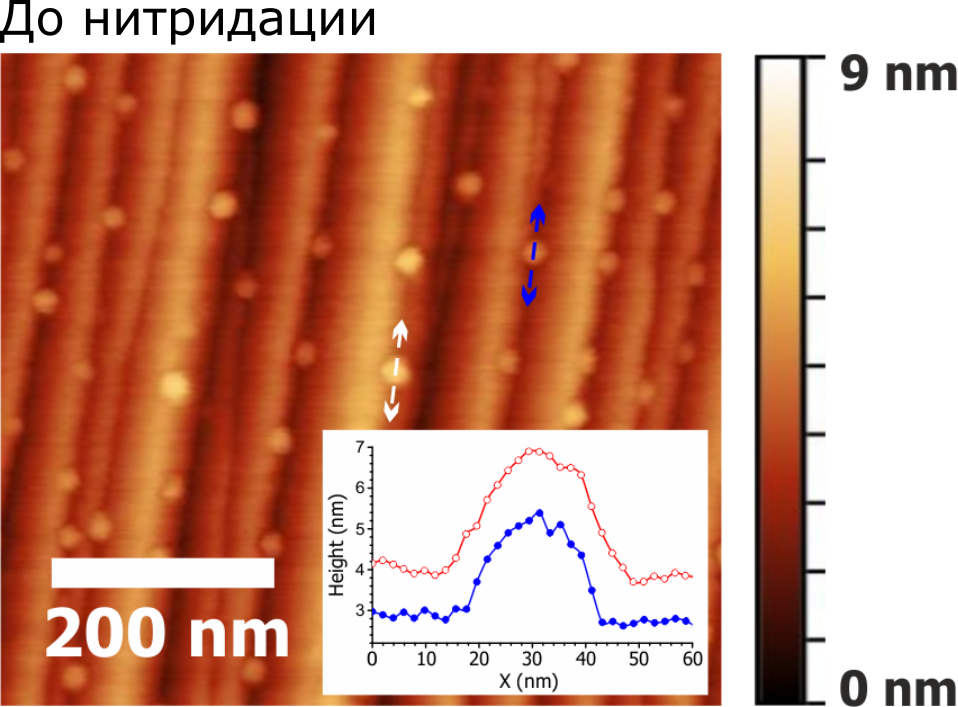
\includegraphics[width=0.45\linewidth]{Image_13_1}}
			\subcaptionbox{\label{fig:Image_13_2}}{%
			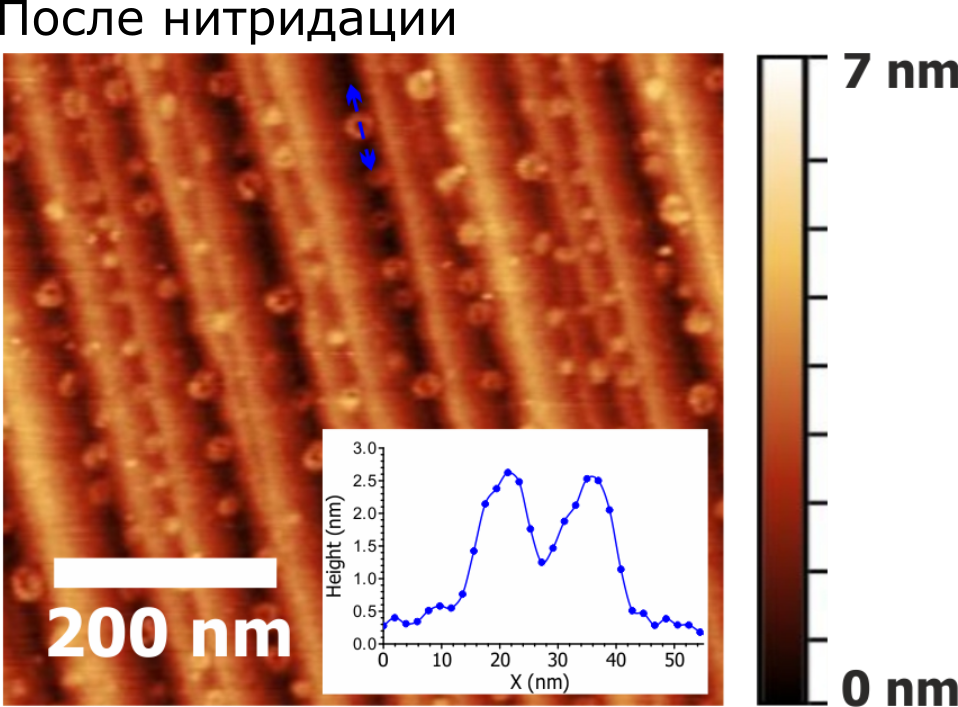
\includegraphics[width=0.45\linewidth]{Image_13_2}} }
			\legend{Разориентация поверхности 4{\textdegree} в направлении <110>. На
				вставках представлены профили АСМ сканирования наноструктур}
				\caption{АСМ изображения поверхности Si подложки с каплями Ga
			(эквивалентной толщины 1,35~монослоя) до нитридации~(а) и после
	нитридации~(б)}\label{fig:Image_13} \end{figure}

Под потоком активированного азота капли кристаллизуются в кольцо высотой
1--2~\si{\nano\meter} и глубиной центрального углубления
0,5--1~\si{\nano\meter} (см. вставки на~рис.~\cref{fig:Image_13}). Схожая
морфология может быть получена капельной эпитаксией GaAs \cite{Zhou2013} и
связана с локализованным ростом соединений
A\textsuperscript{III}B\textsuperscript{V} за счет более быстрого
зародышеобразования вдоль края капли
(см.~подраздел~\cref{subsec:ch1/sec2/sub6}). После нитридации островки обладают
меньшей высотой и повышенной поверхностной плотностью по сравнению с исходными
каплями, что указывает на продолжение диффузия Ga под потоком активного азота.

Исследование ПЭМ не показало травление подложки галлием
(см.~раздел~\cref{subsec:ch3/sec2/sub2}). Морфология поверхности с
нитридированными нанокольцами не изменилась после воздействия водного
раствора соляной кислоты, что указывает на отсутствие металлического Ga или
эвтектического раствора Si-Ga на поверхности после нитридации.

\subsection{Эпитаксиальная ориентация и кристаллическая структура триподов}\label{subsec:ch3/sec2/sub2}

Синтез GaN ННК на подложке с нитридированными каплями Ga может приводить к
формированию дополнительного массива наноструктур~--- ориентированных
наноостровков GaN в форме трипода (см.~рис.~\cref{fig:Image_14_12}).  Триподы
образованы тремя вытянутыми ветвями, расположенными под углом 120{\textdegree}
друг к другу. По отношению к базовому срезу подложки можно определить
эпитаксиальную ориентацию триподов к решётке Si: триподы имеют предпочтительную
ориентацию в плоскости подложки с выравниванием ветвей вдоль
кристаллографических направлений <\(1\overline{1}0\)>\textsubscript{Si},
<\(11\overline{2}\)>\textsubscript{Si}, <\(12\overline{3}\)>\textsubscript{Si}.
Эти ориентации показаны на рисунке~\cref{fig:Image_14_3} с указанием
пунктирными линиями кристаллических двойников, соответствующих повороту на
180{\textdegree} в плоскости подложки. Некоторые триподы имеют только одну или
две ветви.

\begin{figure}[ht] \centerfloat{ \subcaptionbox{\label{fig:Image_14_1}}{%
			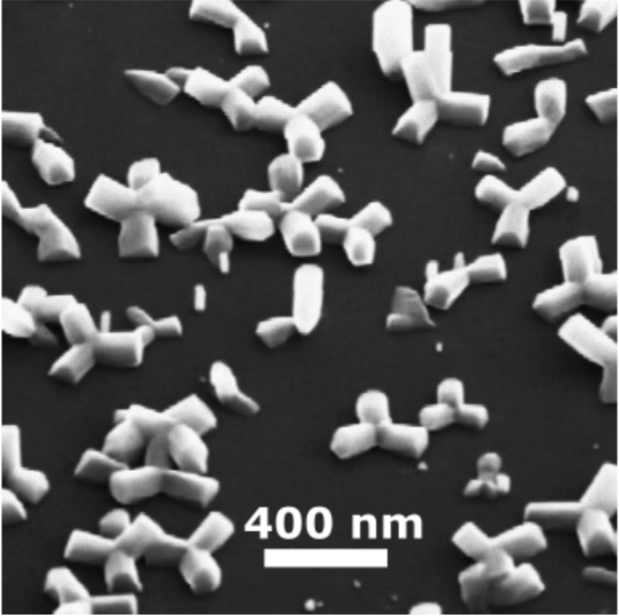
\includegraphics[width=0.4\linewidth]{Image_14_1}}
			\subcaptionbox{\label{fig:Image_14_2}}{%
			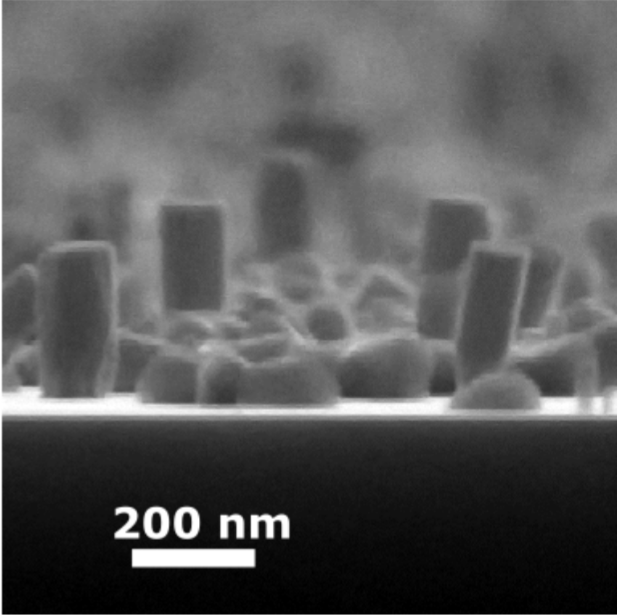
\includegraphics[width=0.4\linewidth]{Image_14_2}} }
			\legend{Изометрический вид~(а), вид сбоку~(б)} \caption{РЭМ изображения
		эпитаксиальных нанотриподов GaN}\label{fig:Image_14_12} \end{figure}

\begin{figure}[ht] \centerfloat{
		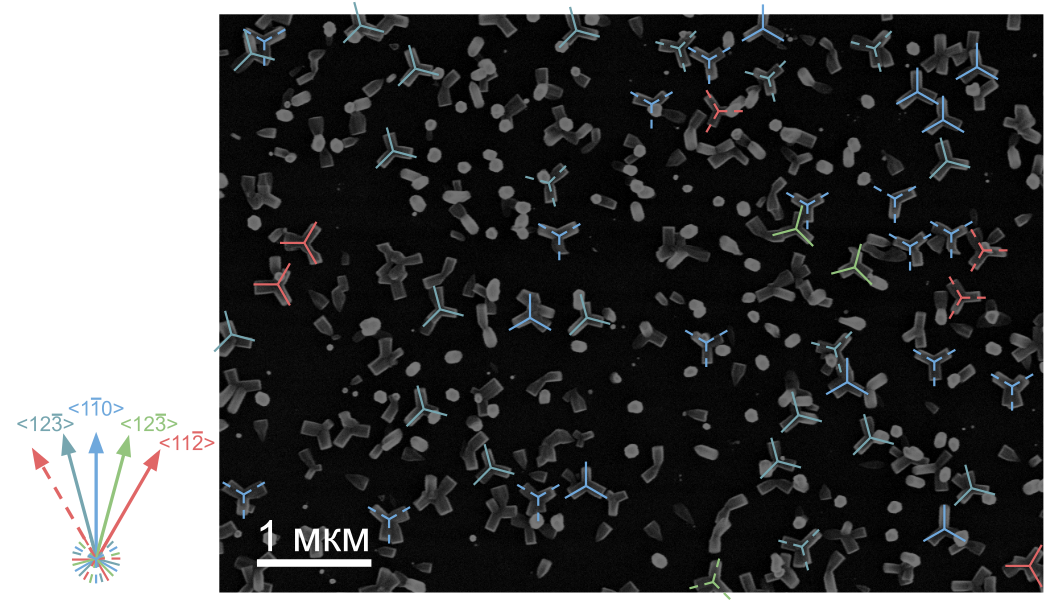
\includegraphics[width=1\linewidth]{Image_14_3} } \legend{Ориентации
		триподов схематически обозначены цветными символами. Кристаллографические
		направления указаны на схеме слева} \caption{РЭМ изображение эпитаксиальных
нанотриподов GaN, вид сверху}\label{fig:Image_14_3} \end{figure}

Формирование подобных GaN триподов уже было исследовано в ряде работ: на
c-плоскости Al\textsubscript{2}O\textsubscript{3} методом хлорид-гидридной
газофазной эпитаксии \cite{Lee2010}, на наноколоннах GaN методом ПА-МПЭ
\cite{Wang2017}, на алмазной подложке методом селективной эпитаксии
\cite{Schuster2015}.

На подложке с поверхностной реконструкцией Si\((111)6,3\)\(\times\)\(6,3 -
\text{Ga}\) синтезирован массив наноструктур (см.~раздел~\cref{sec:ch3/sec1}).
На гетероинтерфейсе GaN/Si (см.~рис.~\cref{fig:Image_15_1}) наблюдается
аморфный слой толщиной \(\approx 1,5\)~\si{\nano\meter}. Данный слой может быть
аморфным SiN\textsubscript{x}, который может формироваться в процессе
нитридации затравочных капель при взаимодействии поверхности Si с активным
азотом. У данного процесса существует несколько механизмов: до насыщения азотом
и образования зародыша капли Ga мигрируют по поверхности Si, которая уже
провзаимодействовала с потоком азота; в процессе насыщения капли Ga часть
растворенных молекул азота взаимодействует с поверхностью подложки под каплей;
адомы азота диффундируют в приповерхностном слое Si \cite{Rawdanowicz2004}.

\begin{figure}[ht] \centerfloat{ \subcaptionbox{\label{fig:Image_15_1}}{%
			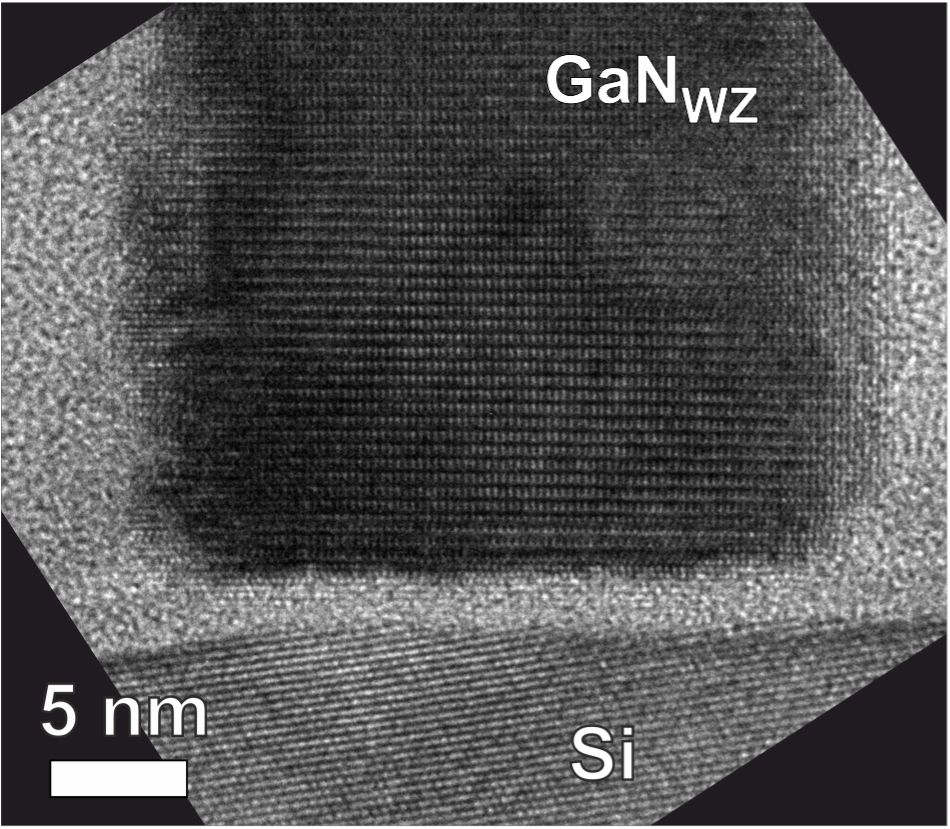
\includegraphics[height=7cm]{Image_15_1}}
			\subcaptionbox{\label{fig:Image_15_2}}{%
			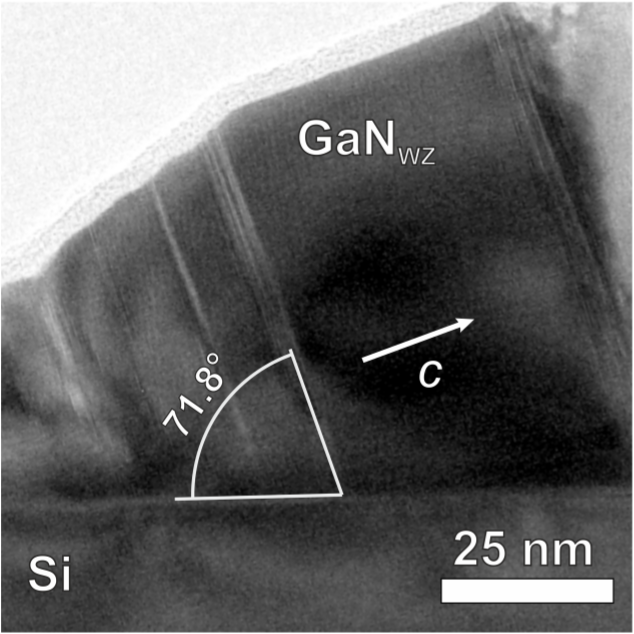
\includegraphics[height=7cm]{Image_15_2}} } \caption{ВРЭМ изображение
		гетероинтерфейса вертикального ННК GaN с подложкой Si(111)~(а), ПЭМ
	изображение ветви трипода GaN на подложке Si(111)~(б)}\label{fig:Image_15}
\end{figure}

Согласно работе \cite{Lee2010}, формирование нанотриподов GaN начинается с
образования ZB наноостровка с последующим зарождением и ростом в плоскости
подложки WZ наностержней на его \{111\} фасетках. Изучение триподов методом ПЭМ
затруднено формированием муарового контраста от наложения решёток ветви и ядра,
поэтому выводы о структуре ядра триподов были сделаны на основе изучения схожих
объектов массива.

При изучении ПЭМ изображений образца были обнаружены наклонный ННК и ветвь
нанотрипода с общим ядром (см.~рис.~\cref{fig:Image_16}). На картинах
электронной микродифракции этих структур были видны рефлексы только WZ
структуры GaN, так как интенсивность рассеяния на ядре наночастицы была
недостаточной для регистрации из-за ее малого объёма.

Упаковка кристаллической решётки WZ и ZB была различима на изображениях ВРЭМ с
ориентацией образца вдоль оси зоны
\([\overline{1}2\overline{1}0]\)\textsubscript{WZ-GaN}. Изображения быстрого
преобразования Фурье (БПФ) от отмеченных пунктирными квадратами областей
наноструктуры с различными упаковками представлены
на~рис.~\cref{fig:Image_16_2}. Расчётные сечения обратного пространства WZ и ZB
структур с соответствующими осями зон
\([\overline{1}2\overline{1}0]\)\textsubscript{WZ-GaN} и
\([\overline{11}0]\)\textsubscript{ZB-GaN} отмечены на изображениях БПФ
оранжевыми и белыми пунктирными кружками соответственно.

\begin{figure}[ht] \centerfloat{ \subcaptionbox{\label{fig:Image_16_1}}{%
			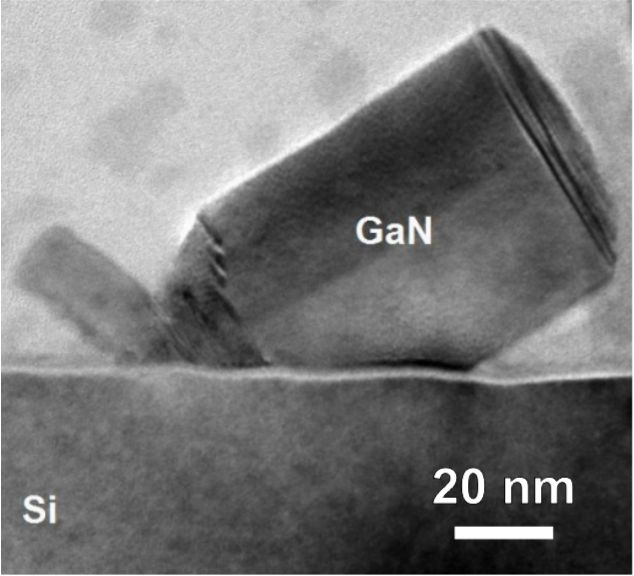
\includegraphics[height=8cm]{Image_16_1}}
			\subcaptionbox{\label{fig:Image_16_2}}{%
			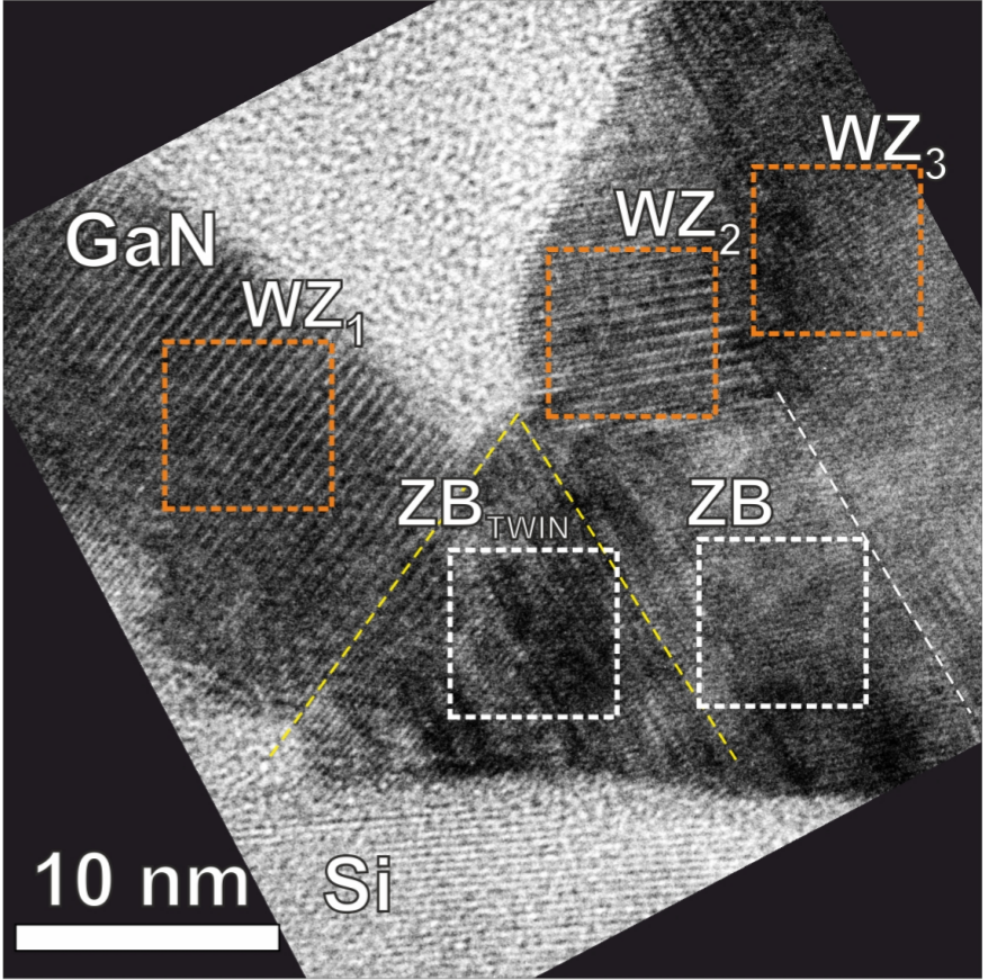
\includegraphics[height=8cm]{Image_16_2}}

		\subcaptionbox{\label{fig:Image_16_3}}{%
			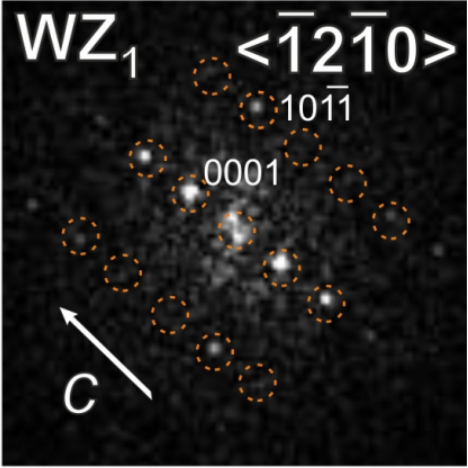
\includegraphics[width=0.19\linewidth]{Image_16_3}}
			\subcaptionbox{\label{fig:Image_16_4}}{%
				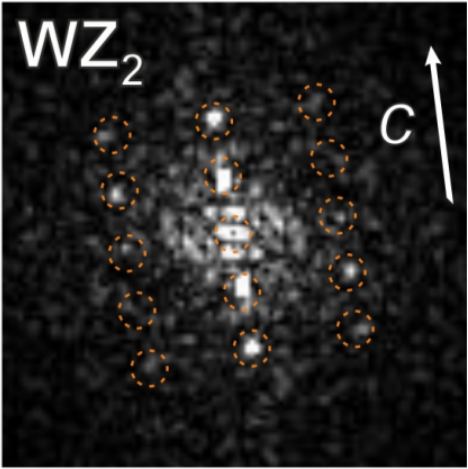
\includegraphics[width=0.19\linewidth]{Image_16_4}}
				\subcaptionbox{\label{fig:Image_16_5}}{%
				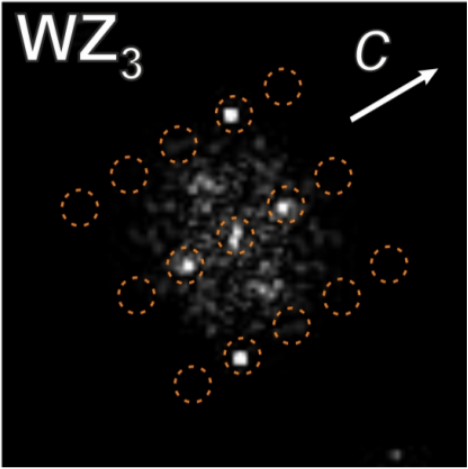
\includegraphics[width=0.19\linewidth]{Image_16_5}}
				\subcaptionbox{\label{fig:Image_16_6}}{%
					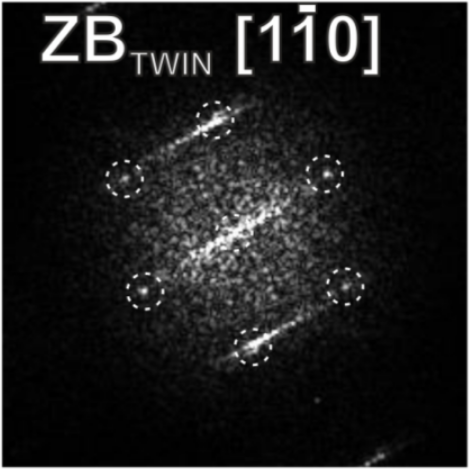
\includegraphics[width=0.19\linewidth]{Image_16_6}}
					\subcaptionbox{\label{fig:Image_16_7}}{%
				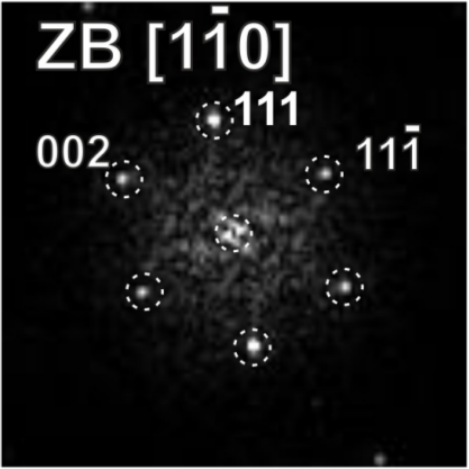
\includegraphics[width=0.19\linewidth]{Image_16_7}} }
				\caption{Микроснимок ПЭМ наклонного ННК и ветви трипода GaN с общим
					центром~(а). Вид крупным планом ВРЭМ~(б) с соответствующими
			изображениями БПФ от областей, отмеченных пунктирными
	квадратами~(в\,--\,ж)}\label{fig:Image_16} \end{figure}

В результате БПФ анализа отчётливо видно отличие кристаллической структуры
основания от ветви и наклонного ННК: наиболее заметное отличие~---
периодичность и симметрия БПФ образа, соответствующая гексагональной и
кубической последовательности укладки плотно упакованных плоскостей
\cite{Jo2018, Bayram2014, Borysiuk2014}. В базовой части (отмечена
на~рис.~\cref{fig:Image_16_2} как ZB и ZB\textsubscript{twin}) периодичность
типа ABCABC{\dots} соответствует GaN со структурой ZB (вдоль <111>). Каждая из
букв A, B и C обозначает бислой атомов, состоящий из одного слоя с атомами
группы III и одного слоя с атомами группы V. У наклонного ННК и ветви
(обозначены на~рис.~\cref{fig:Image_16_2} как WZ\textsubscript{1},
WZ\textsubscript{2}, WZ\textsubscript{3}) периодичность типа ABAB{\dots}
соответствует GaN со структурой WZ (вдоль <0001>) \cite{Kriegner2011}.

Таким образом, WZ триподы и наклонные ННК имеют в основании ZB наноостровок. В
простейшем случае он имеет тетраэдрическую форму с гранями
\{111\}\textsubscript{ZB-GaN}, плоскость (111)\textsubscript{ZB-GaN} которых
ориентирована параллельно Si(111). Такое ZB ядро служит центром
зародышеобразования трипода или наклонённого ННК. Вертикальные ННК
(см.~рис.~\cref{fig:Image_15_1}) не имеют в основании затравочных островков.

Зарождение метастабильной ZB структуры GaN связывают с низкой температурой
роста или избытком Ga \cite{Shi2006, Romano1997}. Аналогичное образование ННК
InAs с метастабильной WZ структурой объясняют размерными эффектами
\cite{Johansson2010}.

Яркие полосы вдоль направления \([11\overline{1}]\) на БПФ образе области
ZB\textsubscript{twin} (см.~рис.~\cref{fig:Image_16_2}) свидетельствуют о
наличии планарных дефектов в плоскости перпендикулярной направлению тяжей.
Главным образом планарные дефекты~--- это кристаллические двойникования,
соответствующие повороту на 180{\textdegree} вокруг направления
\([11\overline{1}]\)\textsubscript{ZB-GaN}. Подобное двойникование может
происходить вокруг любого направления <111> \cite{Suturin2017} и приводить к
формированию двойниковой \{111\}\textsubscript{ZB-GaN} грани внутри одного ZB
островка (см.~подраздел~\cref{subsec:ch1/sec2/sub5}). Ориентация таких граней
определяет направление роста наклонных ННК.

Линейные контрастные особенности на ПЭМ изображениях ветвей трипода
на~рисунках~\cref{fig:Image_16_1}~и~\cref{fig:Image_15_2} связаны с двумерными
дефектами, перпендикулярными направлению (0001)\textsubscript{WZ-GaN}
(см.~подраздел~\cref{subsec:ch1/sec2/sub5}). Преимущественно это дефекты
упаковки.

Угол между плоскостью Si(111) и (0001)\textsubscript{WZ-GaN} ветви трипода,
изображённом на~рис.~\cref{fig:Image_15_2} составляет \(72\si{\degree} \pm
1\si{\degree}\), что соответствует значению угла между плоскостями
(0001)\textsubscript{WZ-GaN} и \((11\overline{2}1)\)\textsubscript{WZ-GaN}
(72,92\textdegree) \cite{Wang2016}. Таким образом, кристаллографическая
плоскость \((11\overline{2}1)\)\textsubscript{WZ-GaN} ветвей триподов GaN
параллельна поверхности подложки Si(111).

На другом образце с эквивалентной толщиной затравочного Ga в 2~монослоя
наблюдались двойные наклонные ННК (см.~рис.~\cref{fig:Image_18}). На
изображении ВРЭМ (см.~рис.~\cref{fig:Image_18_2}) наблюдается общее ZB ядро
двойных наклонных ННК. Из БПФ образов заметно, что в отличии от предыдущего
случая, грань (001)\textsubscript{ZB-GaN} ядра ориентирована перпендикулярно
плоскости подложки Si(111). Подобная морфология наблюдалась в работе
\cite{Wang2017}.

\begin{figure}[ht] \centerfloat{ \subcaptionbox{\label{fig:Image_18_1}}{%
			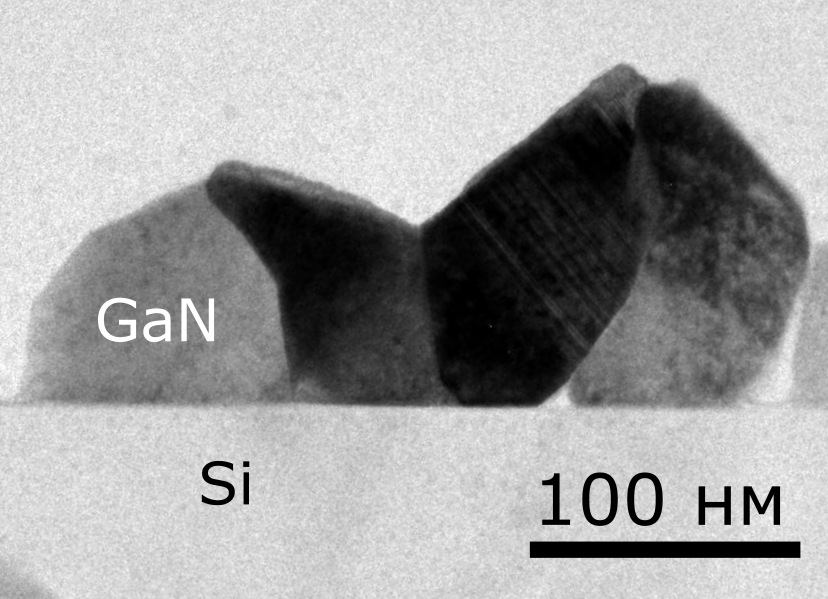
\includegraphics[height=7cm]{Image_18_1}}
			\subcaptionbox{\label{fig:Image_18_2}}{%
			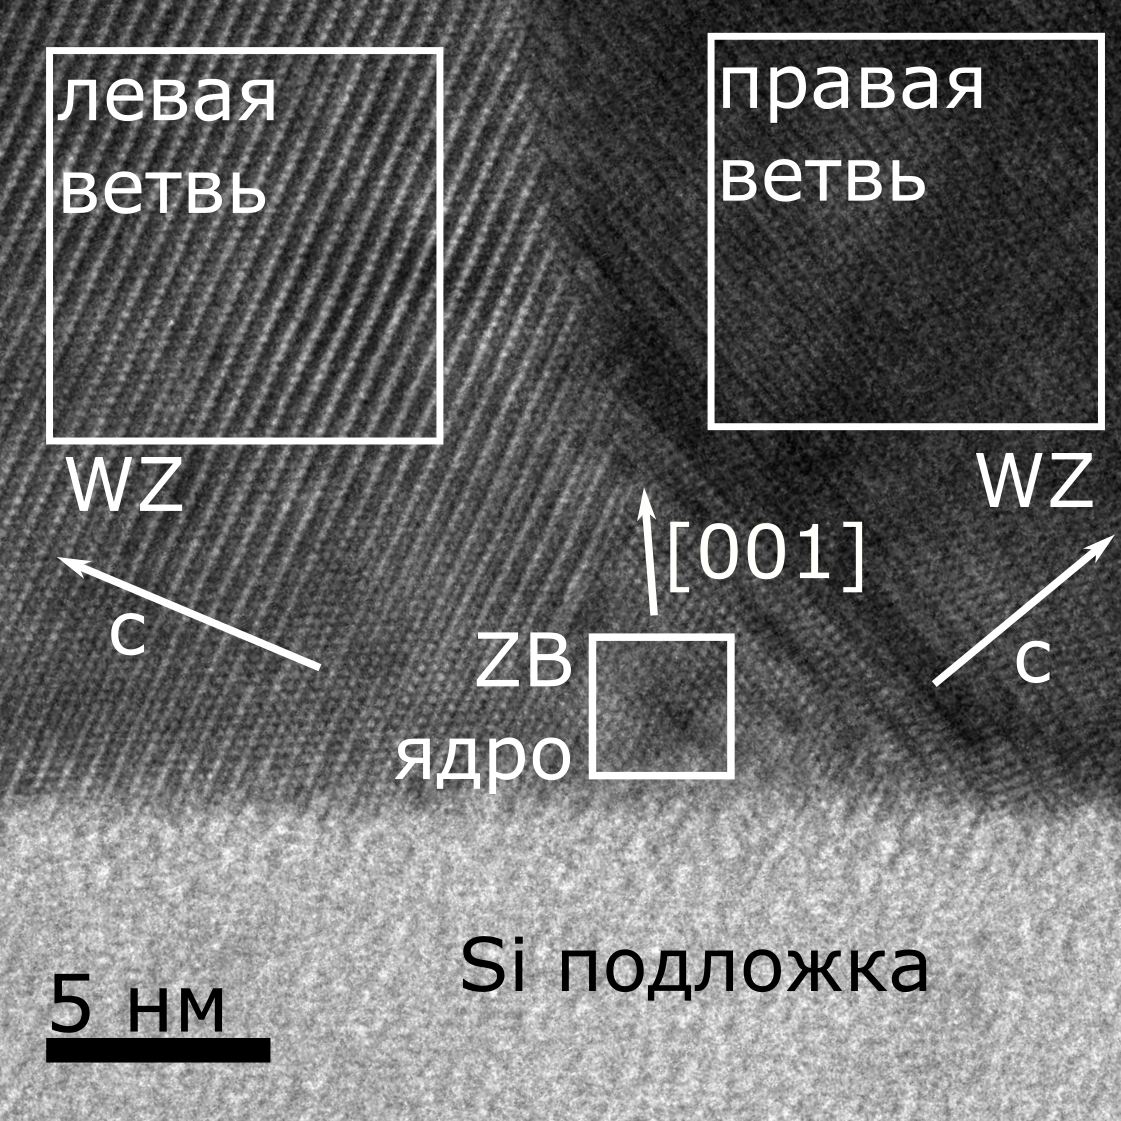
\includegraphics[height=7cm]{Image_18_2}}

		\subcaptionbox{\label{fig:Image_18_3}}{%
			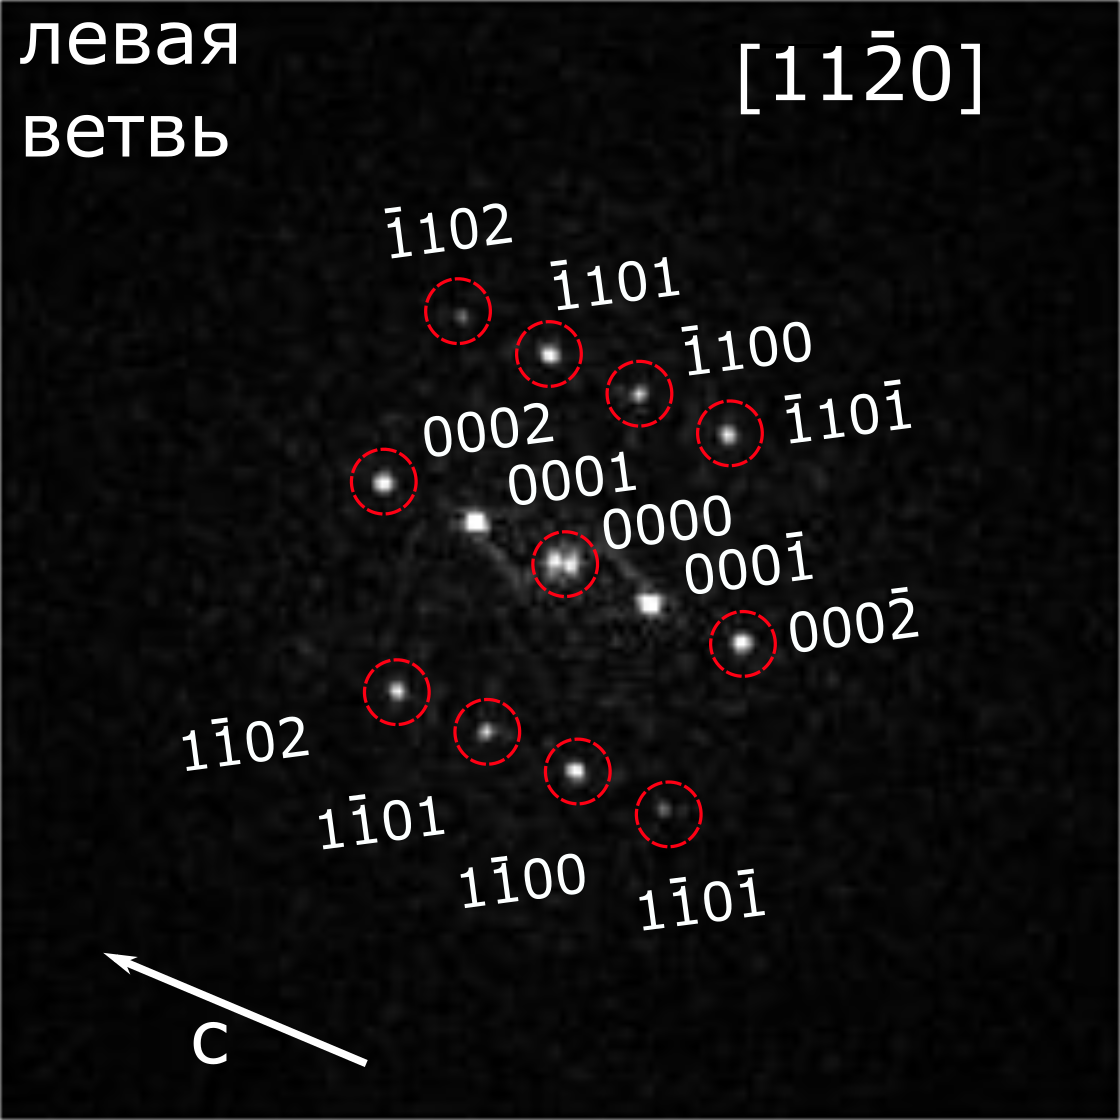
\includegraphics[width=0.31\linewidth]{Image_18_3}}
			\subcaptionbox{\label{fig:Image_18_4}}{%
				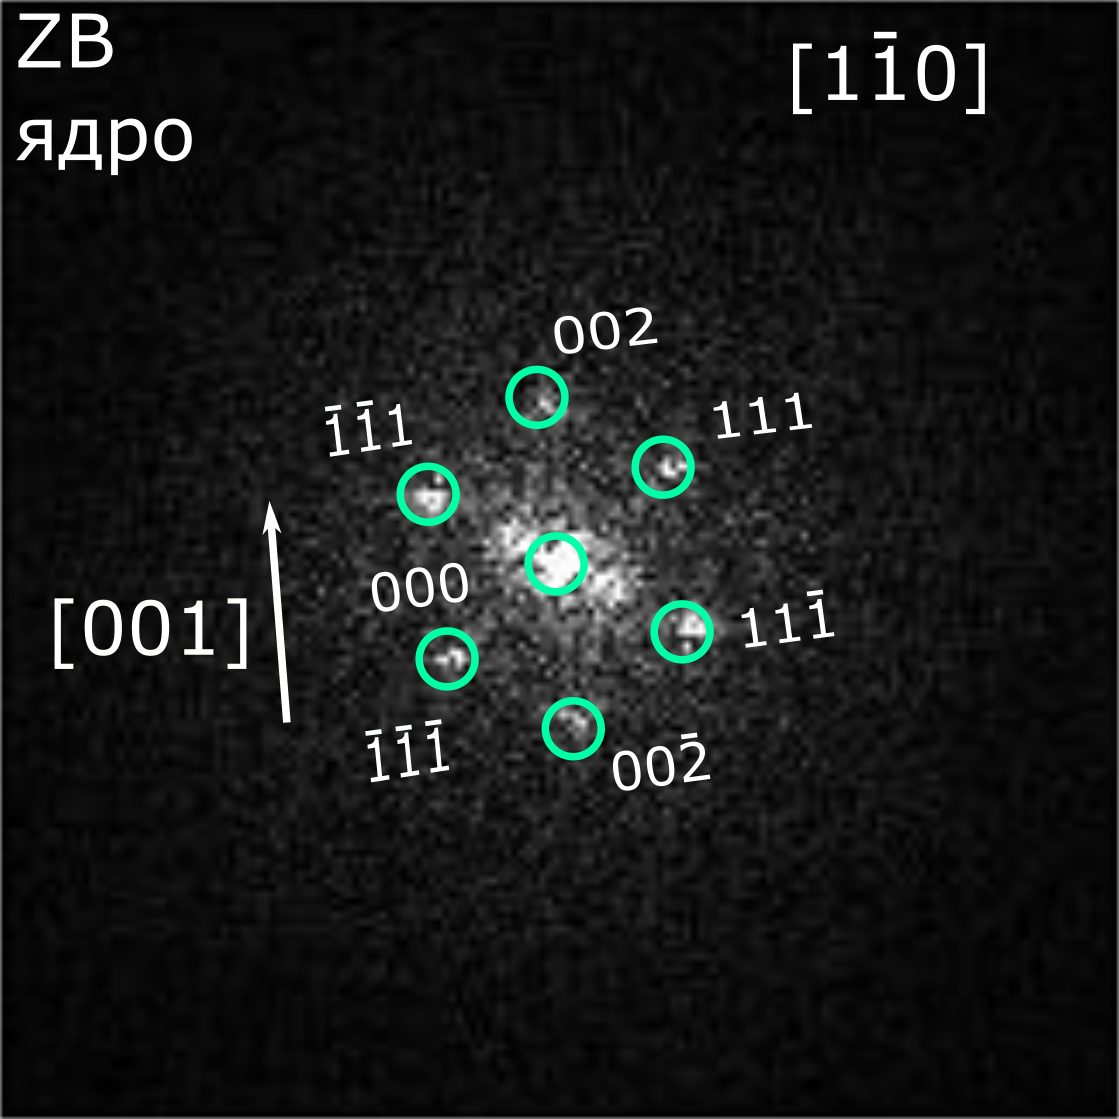
\includegraphics[width=0.31\linewidth]{Image_18_4}}
				\subcaptionbox{\label{fig:Image_18_5}}{%
				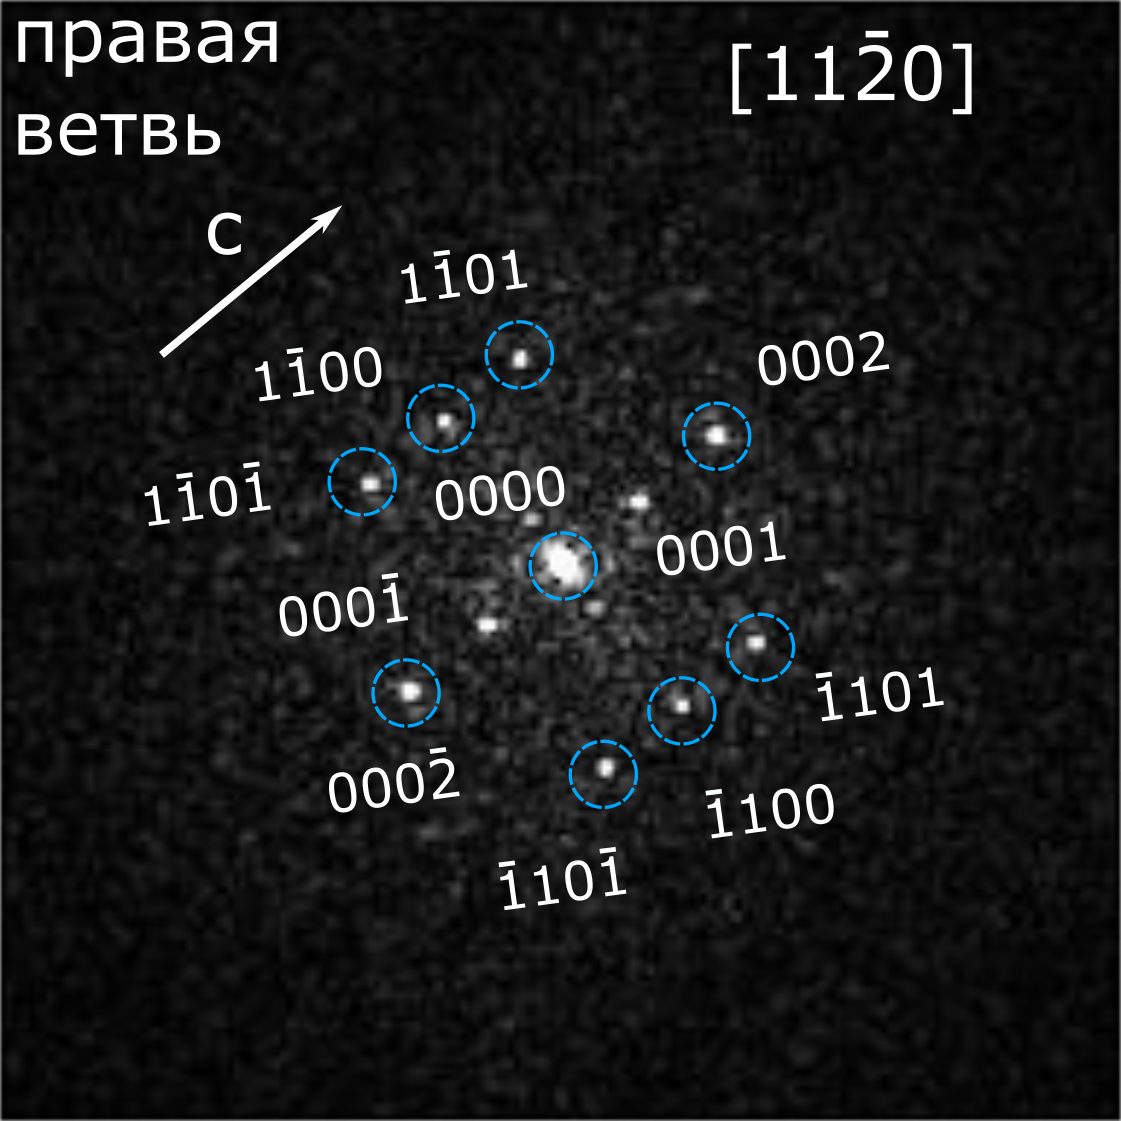
\includegraphics[width=0.31\linewidth]{Image_18_5}} } \caption{ПЭМ
				изображение наклонных ННК GaN с общим ядром~(а). Вид крупным планом
				ВРЭМ~(б) с соответствующими изображениями БПФ от отмеченных квадратами
		областей~(в\,--\,д)}\label{fig:Image_18} \end{figure}

\{111\}\textsubscript{ZB-GaN} ядра служат центрами зародышеобразования WZ ННК.
Угол между осями сросшихся ННК \(\approx 116\){\textdegree} (угол между [111] и
\([\overline{111}]\) составляет 109,47\textdegree), что указывает на
формирование \([\overline{1}103]\)\textsubscript{WZ-GaN} плоскости сращивания,
а не ожидаемой \([\overline{3}308]\)\textsubscript{WZ-GaN}.

Подводя итог, триподы и наклонные ННК имеют в основании ZB ядро, а их
морфология зависит от кристаллографической ориентации и возможных
кристаллических двойникований ядра.

\subsection{Исследование ФЛ триподов}\label{subsec:ch3/sec2/sub3}

Для исследования ФЛ был выбран образец с высокой поверхностной плотностью
триподов \((\approx 20~\si{\micro\meter^{-2}})\). Измерения проводились при
температуре 10~\si{\kelvin} с возбуждением на длине волны 325~\si{\nano\meter}
непрерывным HeCd лазером. Типичный спектр ФЛ ансамбля нанотриподов GaN
(см.~рис.~\cref{fig:Image_19}) имеет три полосы: A (\(\approx
3,48\)~\si{\electronvolt}), B (\(\approx 3,43\)~\si{\electronvolt}) и C
(\(\approx 3,25\)~\si{\electronvolt)}.

\begin{figure}[ht] \centerfloat{
		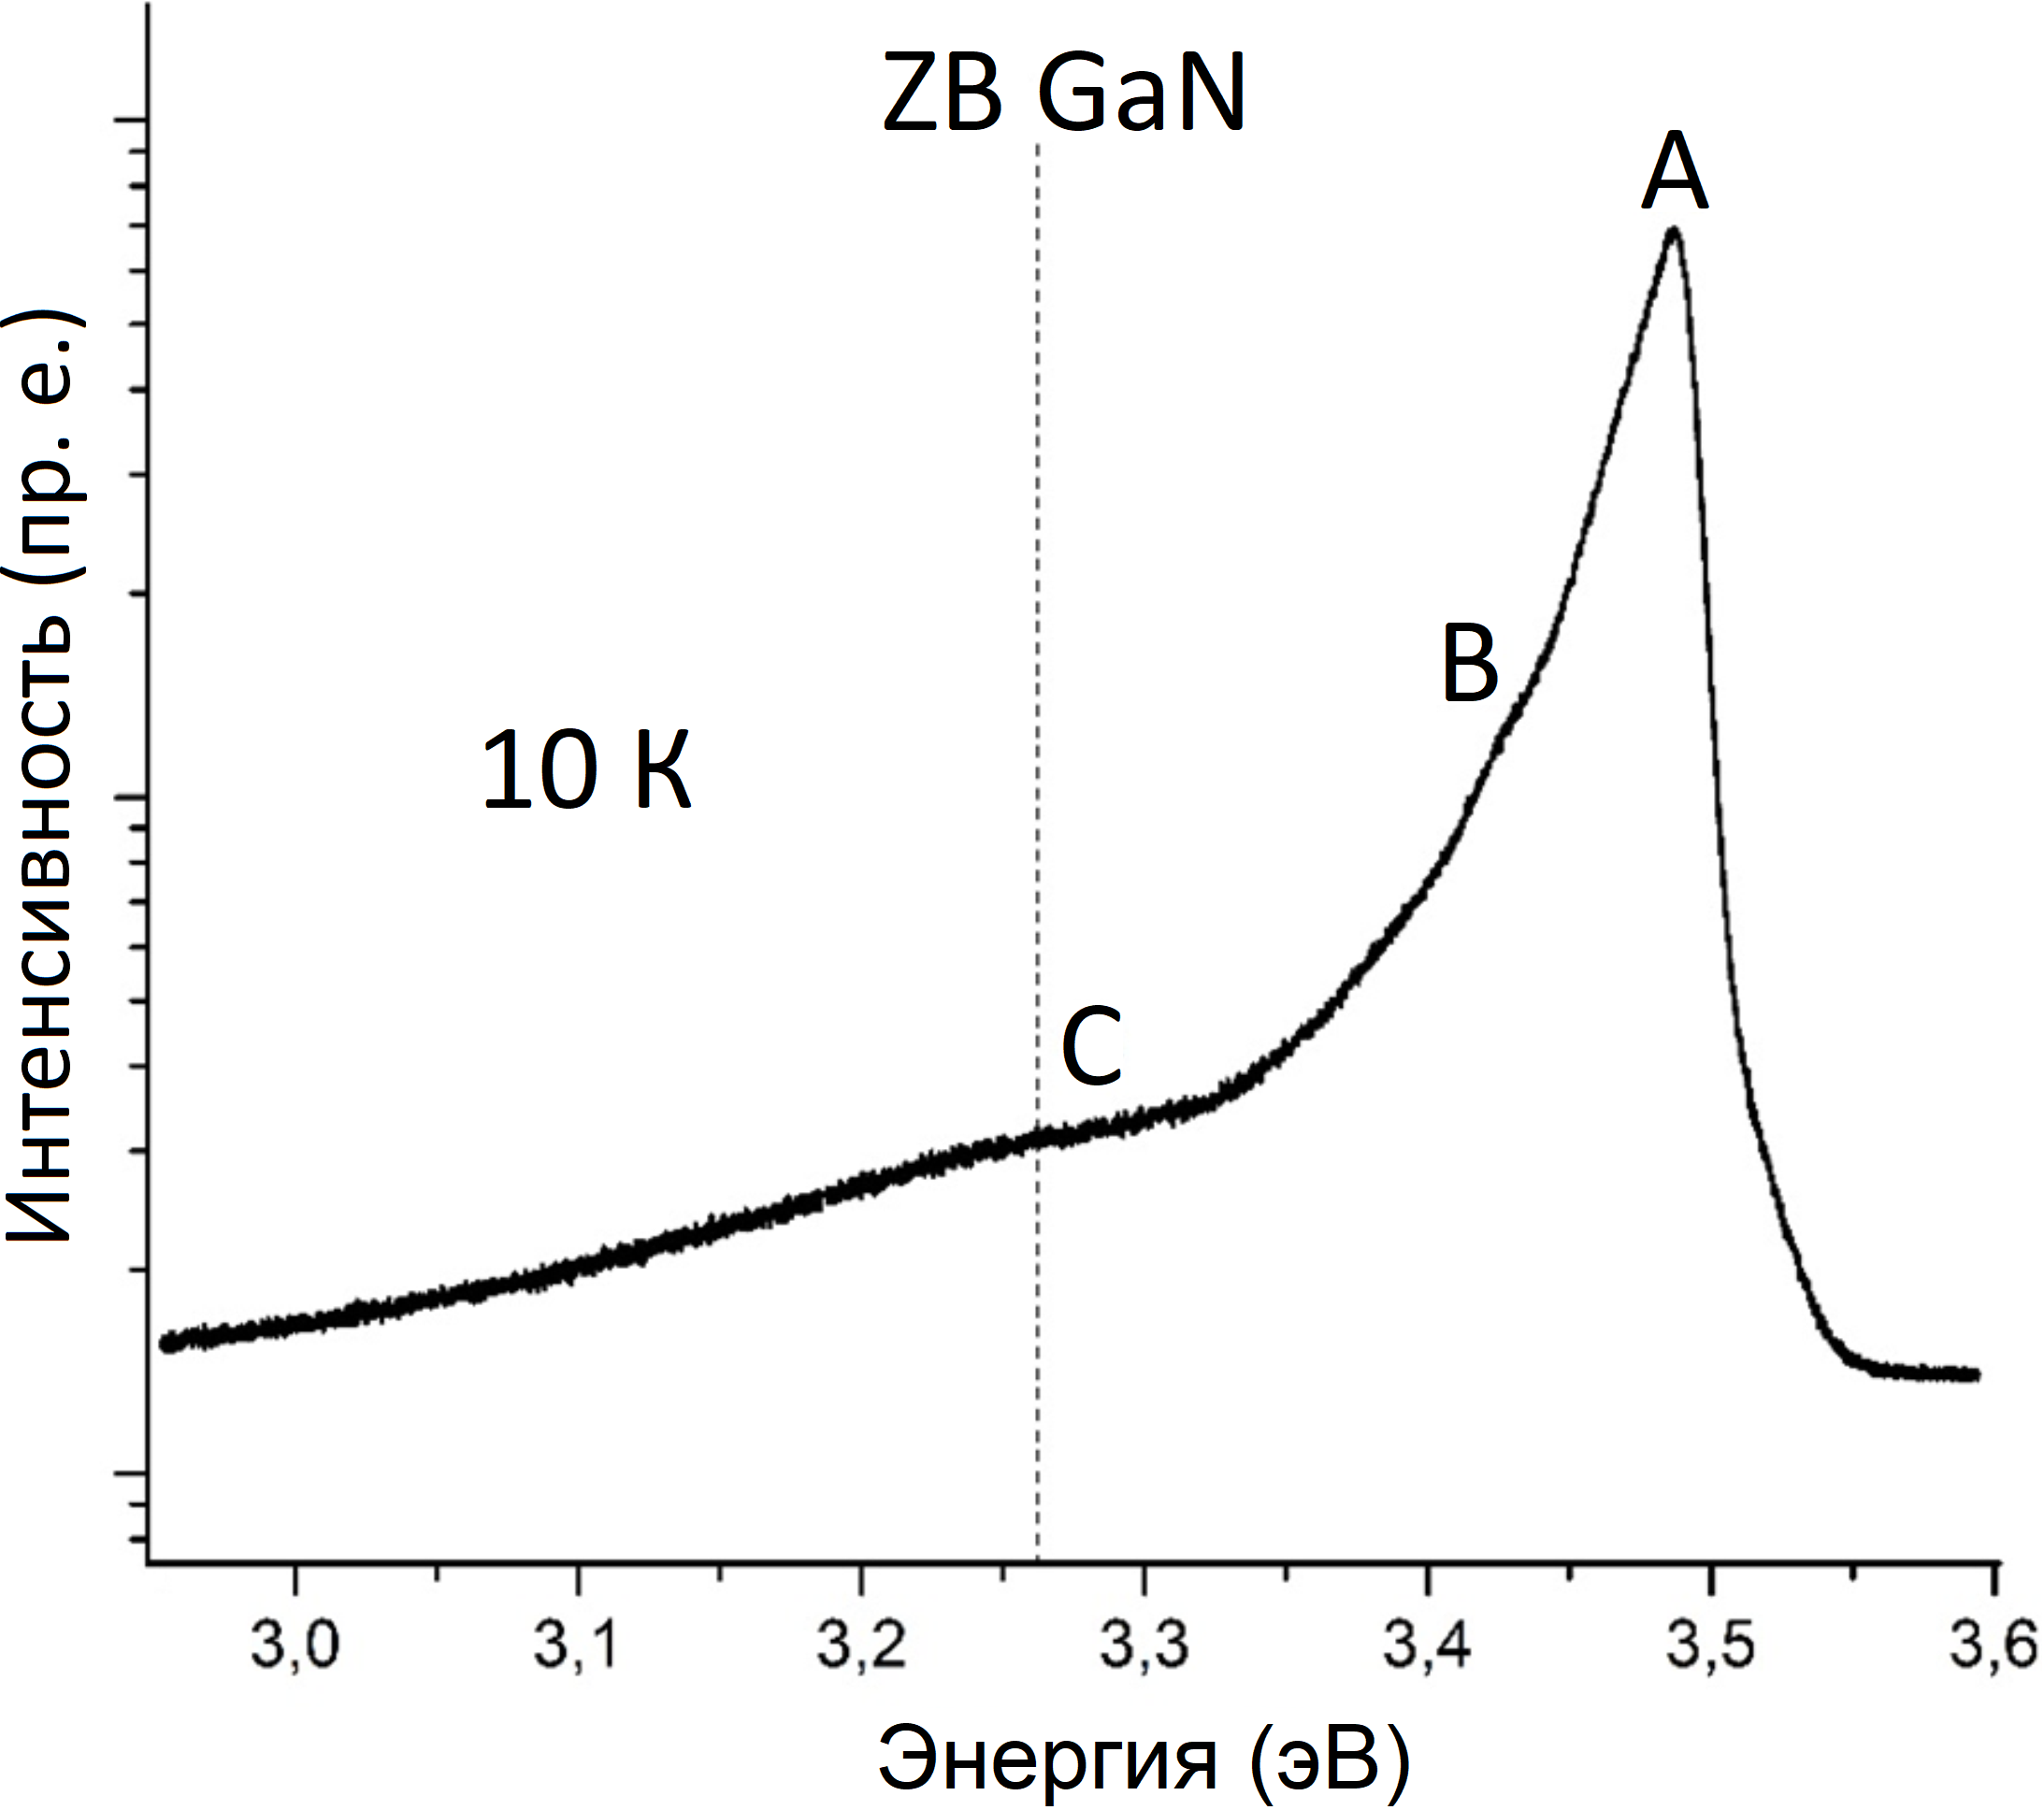
\includegraphics[width=0.5\linewidth]{Image_19} } \legend{Морфология
		поверхности образца изображена на~рисунке~\cref{fig:Image_25_1}, спектр
		снят при температуре 10~\si{\kelvin}} \caption{Низкотемпературный спектр ФЛ
		массива эпитаксиальных триподов GaN с высокой поверхностной
плотностью}\label{fig:Image_19} \end{figure}

Полоса A характерна для объёмного GaN со структурой WZ и соответствует
излучению вблизи края поглощения, что может быть связано со связанными на
нейтральном доноре экситонами \cite{Bolshakov2018, Richter2008, Agekyan2013}.

Полоса B может быть связана со структурными дефектами \cite{Calleja2000}, в
частности с наблюдаемыми дефектами упаковки в триподах
(см.~рис.~\cref{fig:Image_15_2}) \cite{Albrecht1997, Paskov2005}. В
Ni-каталитических ННК подобный пик вызван примесями Ni или наличием Ga вакансий
в структуре \cite{Yoo2006}.

Широкая полоса C может быть вызвана включениями ZB в GaN, так как ZB-GaN при
низких температурах излучает вблизи края поглощения с энергией \(\approx
3,27\)~\si{\electronvolt} \cite{Jacobs2007}.

\subsection{Влияние ростовых условий на морфологию наноструктур}\label{subsec:ch3/sec2/sub4}

Наноструктуры для анализа влияния эквивалентной толщины затравочных капель на
морфологию были синтезированы наноструктуры при следующих условиях роста: ЭДП
Ga \(1 \cdot 10^{-8}\)~\si{\torr}, расход азота
0,4~\si{\centi\meter^3\per\minute} и мощность плазменного источника
500~\si{\watt}.

Из сравнения образцов с нитридированными каплями различной эквивалентной
толщины (см.~рис.~\cref{fig:Image_20}) видно, что в исследуемом диапазоне
увеличение количества предварительно осаждённого Ga повышает плотность
затравочных островков GaN, но слабо влияет на их латеральный размер и
морфологию.

\begin{figure}[ht] \centerfloat{ \subcaptionbox{\label{fig:Image_20_1}}{%
			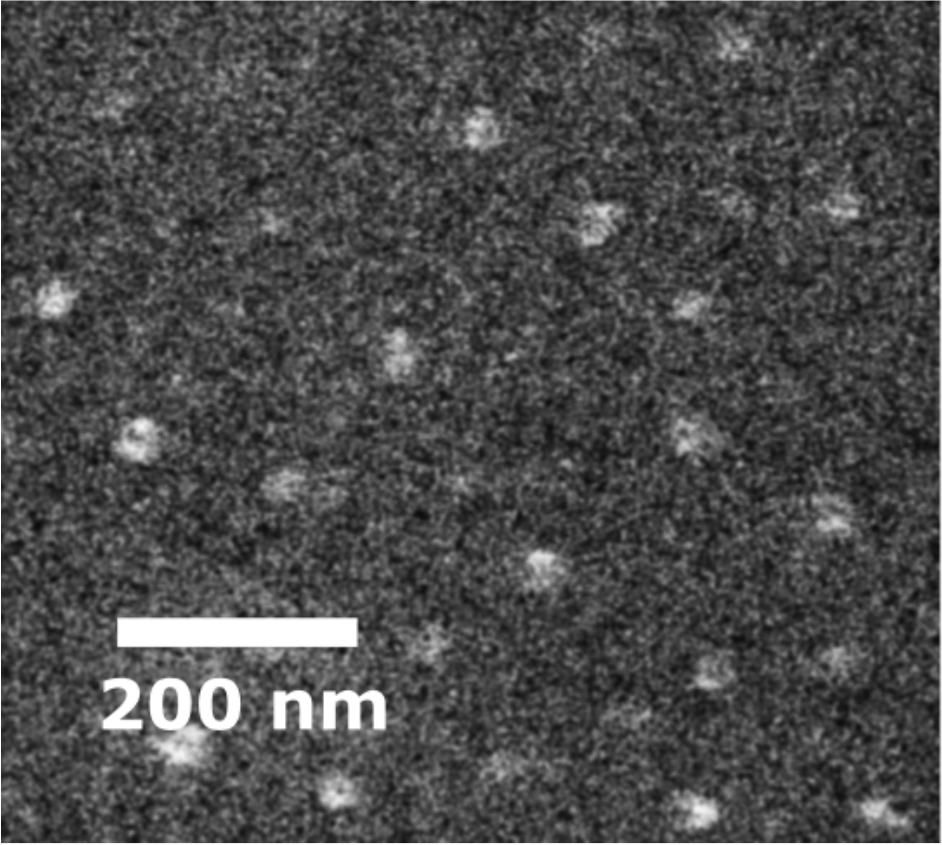
\includegraphics[width=0.25\linewidth]{Image_20_1}}
			\subcaptionbox{\label{fig:Image_20_2}}{%
			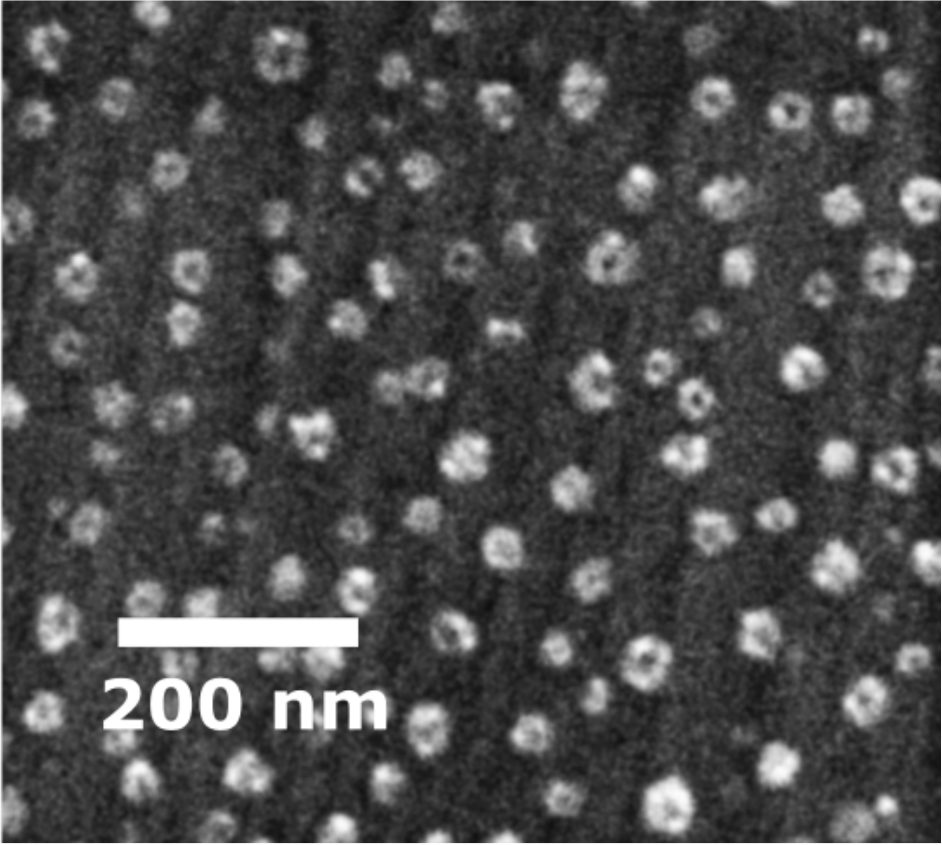
\includegraphics[width=0.25\linewidth]{Image_20_2}} }
			\legend{Эквивалентная толщиной капель Ga 1,35~(а) и 2~монослоя~(б)}
			\caption{РЭМ изображения затравочных островков GaN, выращенных методом
				капельной эпитаксии с различной эквивалентной толщиной капель
		Ga}\label{fig:Image_20} \end{figure}

Затравка Ga с эквивалентной толщиной менее 1~монослоя образует поверхностную
реконструкцию (см.~подраздел~\cref{subsec:ch2/sec1/sub2}), поэтому после
нитридации ZB островки не образуются. Следовательно, формирование триподов
подавляется, образуются исключительно ННК (см.~рис.~\cref{fig:Image_21}).

\begin{figure}[ht] \centerfloat{ \subcaptionbox{\label{fig:Image_21_1}}{%
			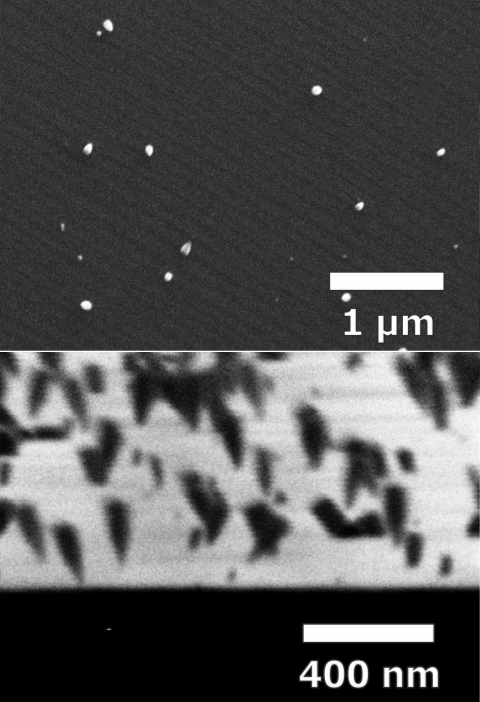
\includegraphics[width=0.25\linewidth]{Image_21_1}}
			\subcaptionbox{\label{fig:Image_21_2}}{%
			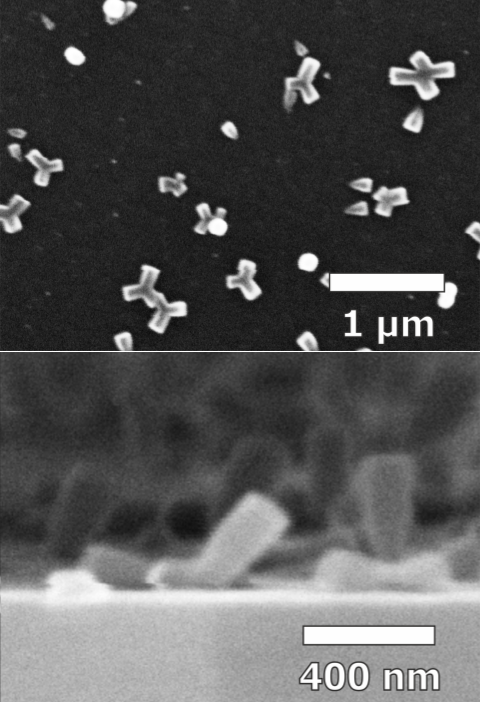
\includegraphics[width=0.25\linewidth]{Image_21_2}} }
			\legend{Эквивалентная толщина Ga 0,7~(а) и 2~монослоя~(б)} \caption{РЭМ
				изображения морфологии наноструктур GaN, синтезированных на затравочных
				островках различной эквивалентной толщины}\label{fig:Image_21}
			\end{figure}

Увеличение эквивалентной толщины затравки в диапазоне 0,7--1,4~монослоя
приводит к увеличению поверхностной плотности затравочных островков, а вместе с
тем увеличивает плотность и эквивалентную толщину синтезированных нанотриподов
(см.~рис.~\cref{fig:Image_22}).

\begin{figure}[ht] \centerfloat{ \subcaptionbox{\label{fig:Image_22_1}}{%
			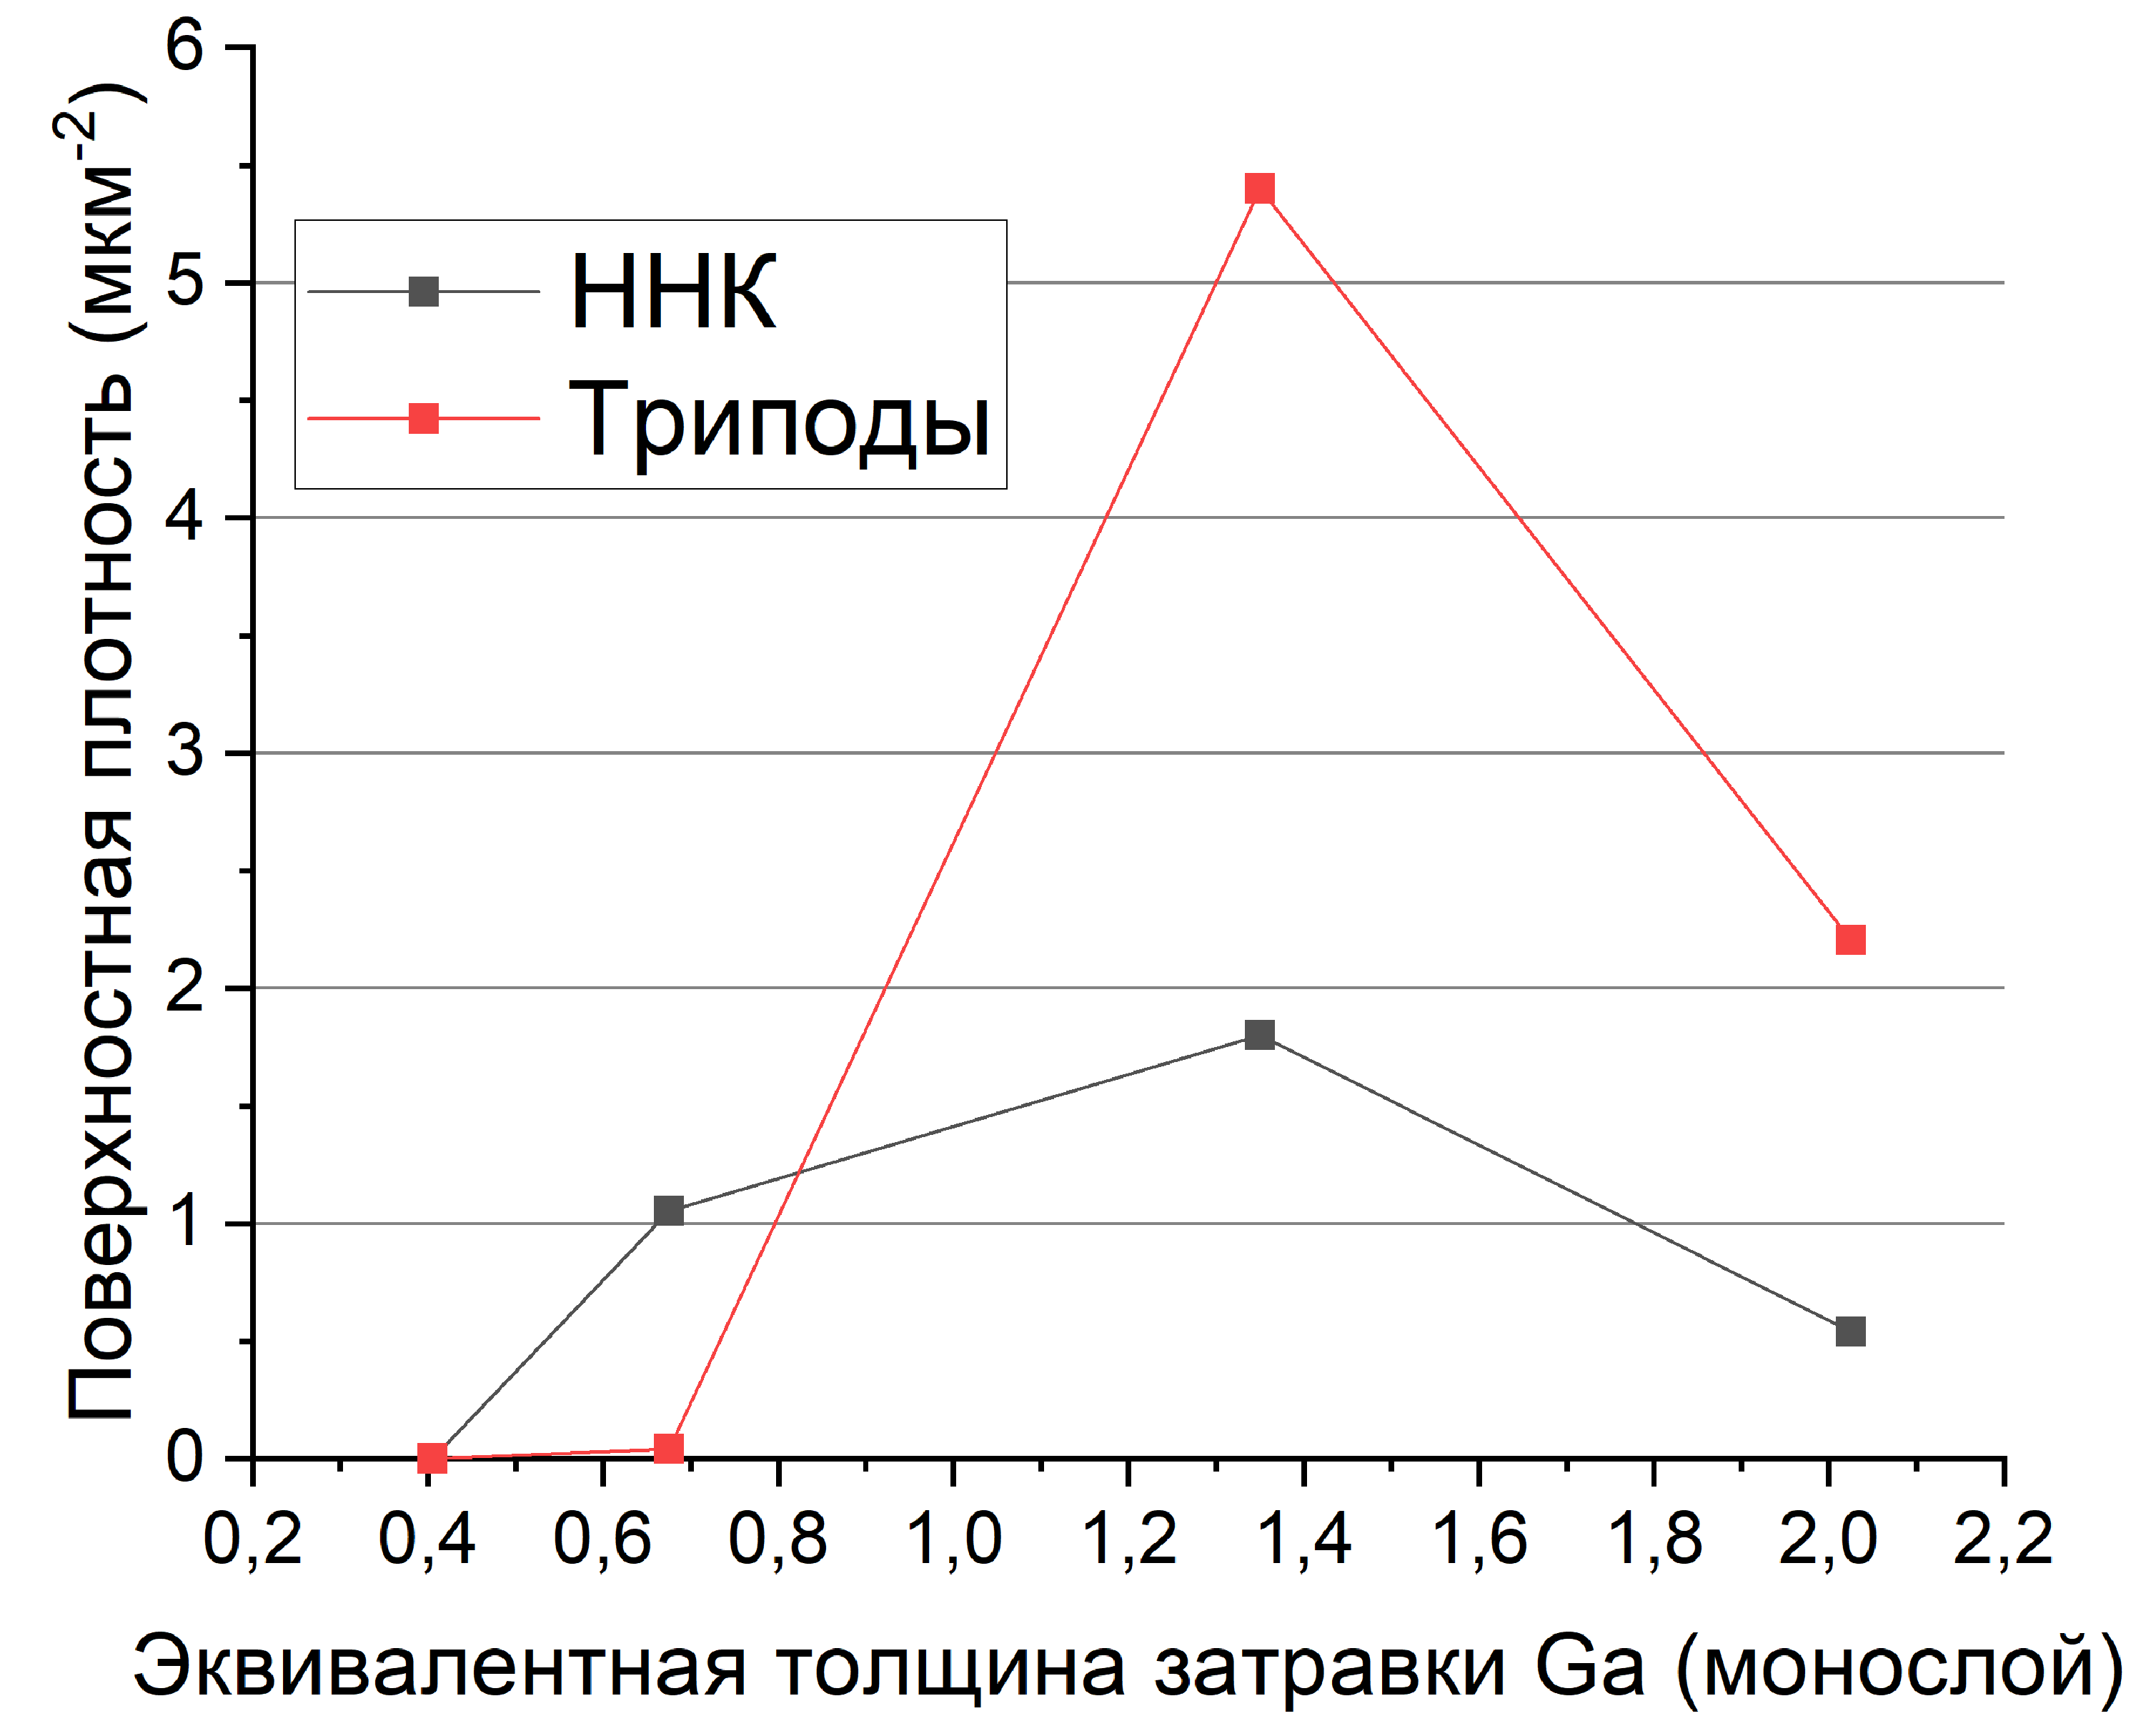
\includegraphics[width=0.48\linewidth]{Image_22_1}}
			\subcaptionbox{\label{fig:Image_22_2}}{%
			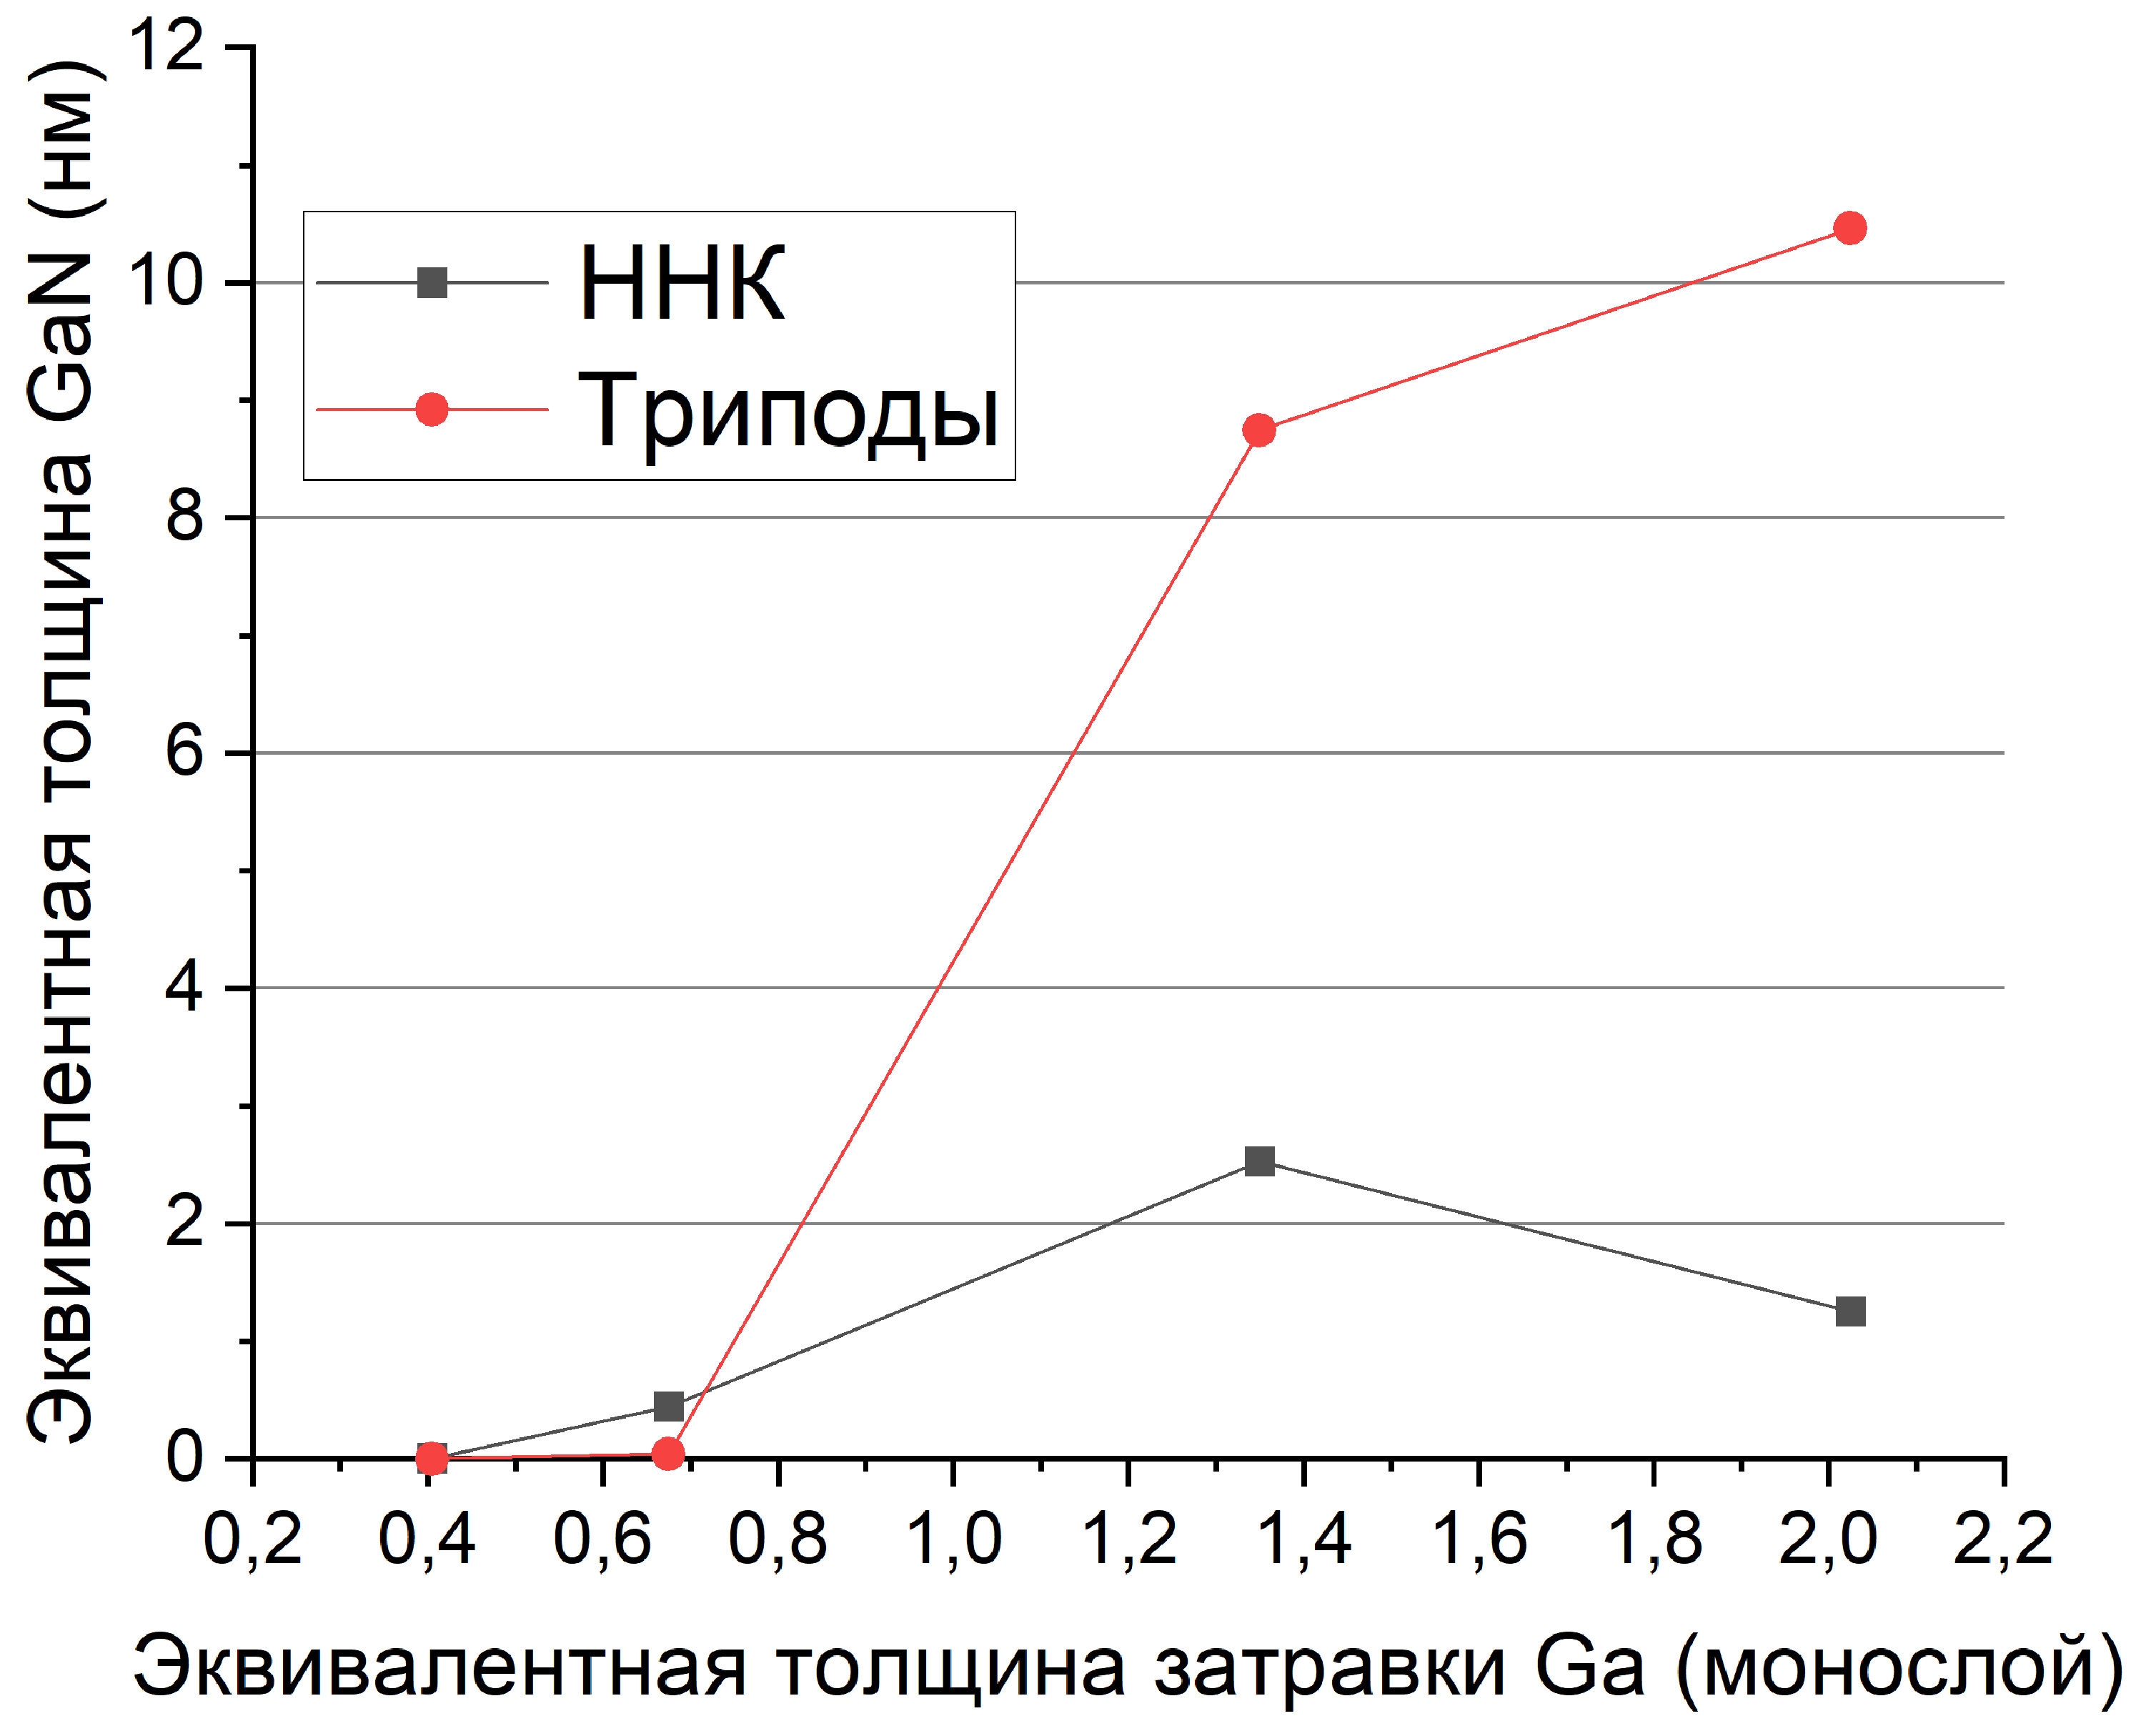
\includegraphics[width=0.48\linewidth]{Image_22_2}} }
			\caption{Зависимости эквивалентной толщины~(а) синтезированного материала
				и поверхностной плотности~(б) массива наноструктур GaN от эквивалентной
				толщины затравочных островков}\label{fig:Image_22} \end{figure}

Эквивалентная толщина синтезированного массива насыщается с дальнейшим
увеличением эквивалентной толщины затравочных капель. Высокая поверхностная
плотность затравочных наноостровков, служащих центрами зародышеобразования,
приводит к слиянию наноструктур массива при дальнейшем росте. Это объясняет
внезапное падение поверхностных плотностей массивов при толщине затравочного
слоя более 1,7~монослоя (см.~рис.~\cref{fig:Image_22}). Использование
затравочных капель с эквивалентной толщиной более 2,4~монослоя приводит к
формированию двумерного слоя GaN из сросшихся островков.

Для изучения влияния соотношения V/III на формирование триподов проведена
ростовая серия с образцами, синтезированными при различных ЭДП Ga
(см.~рис.~\cref{fig:Image_23}).

\begin{figure}[ht] \centerfloat{ \subcaptionbox{\label{fig:Image_23_1}}{%
			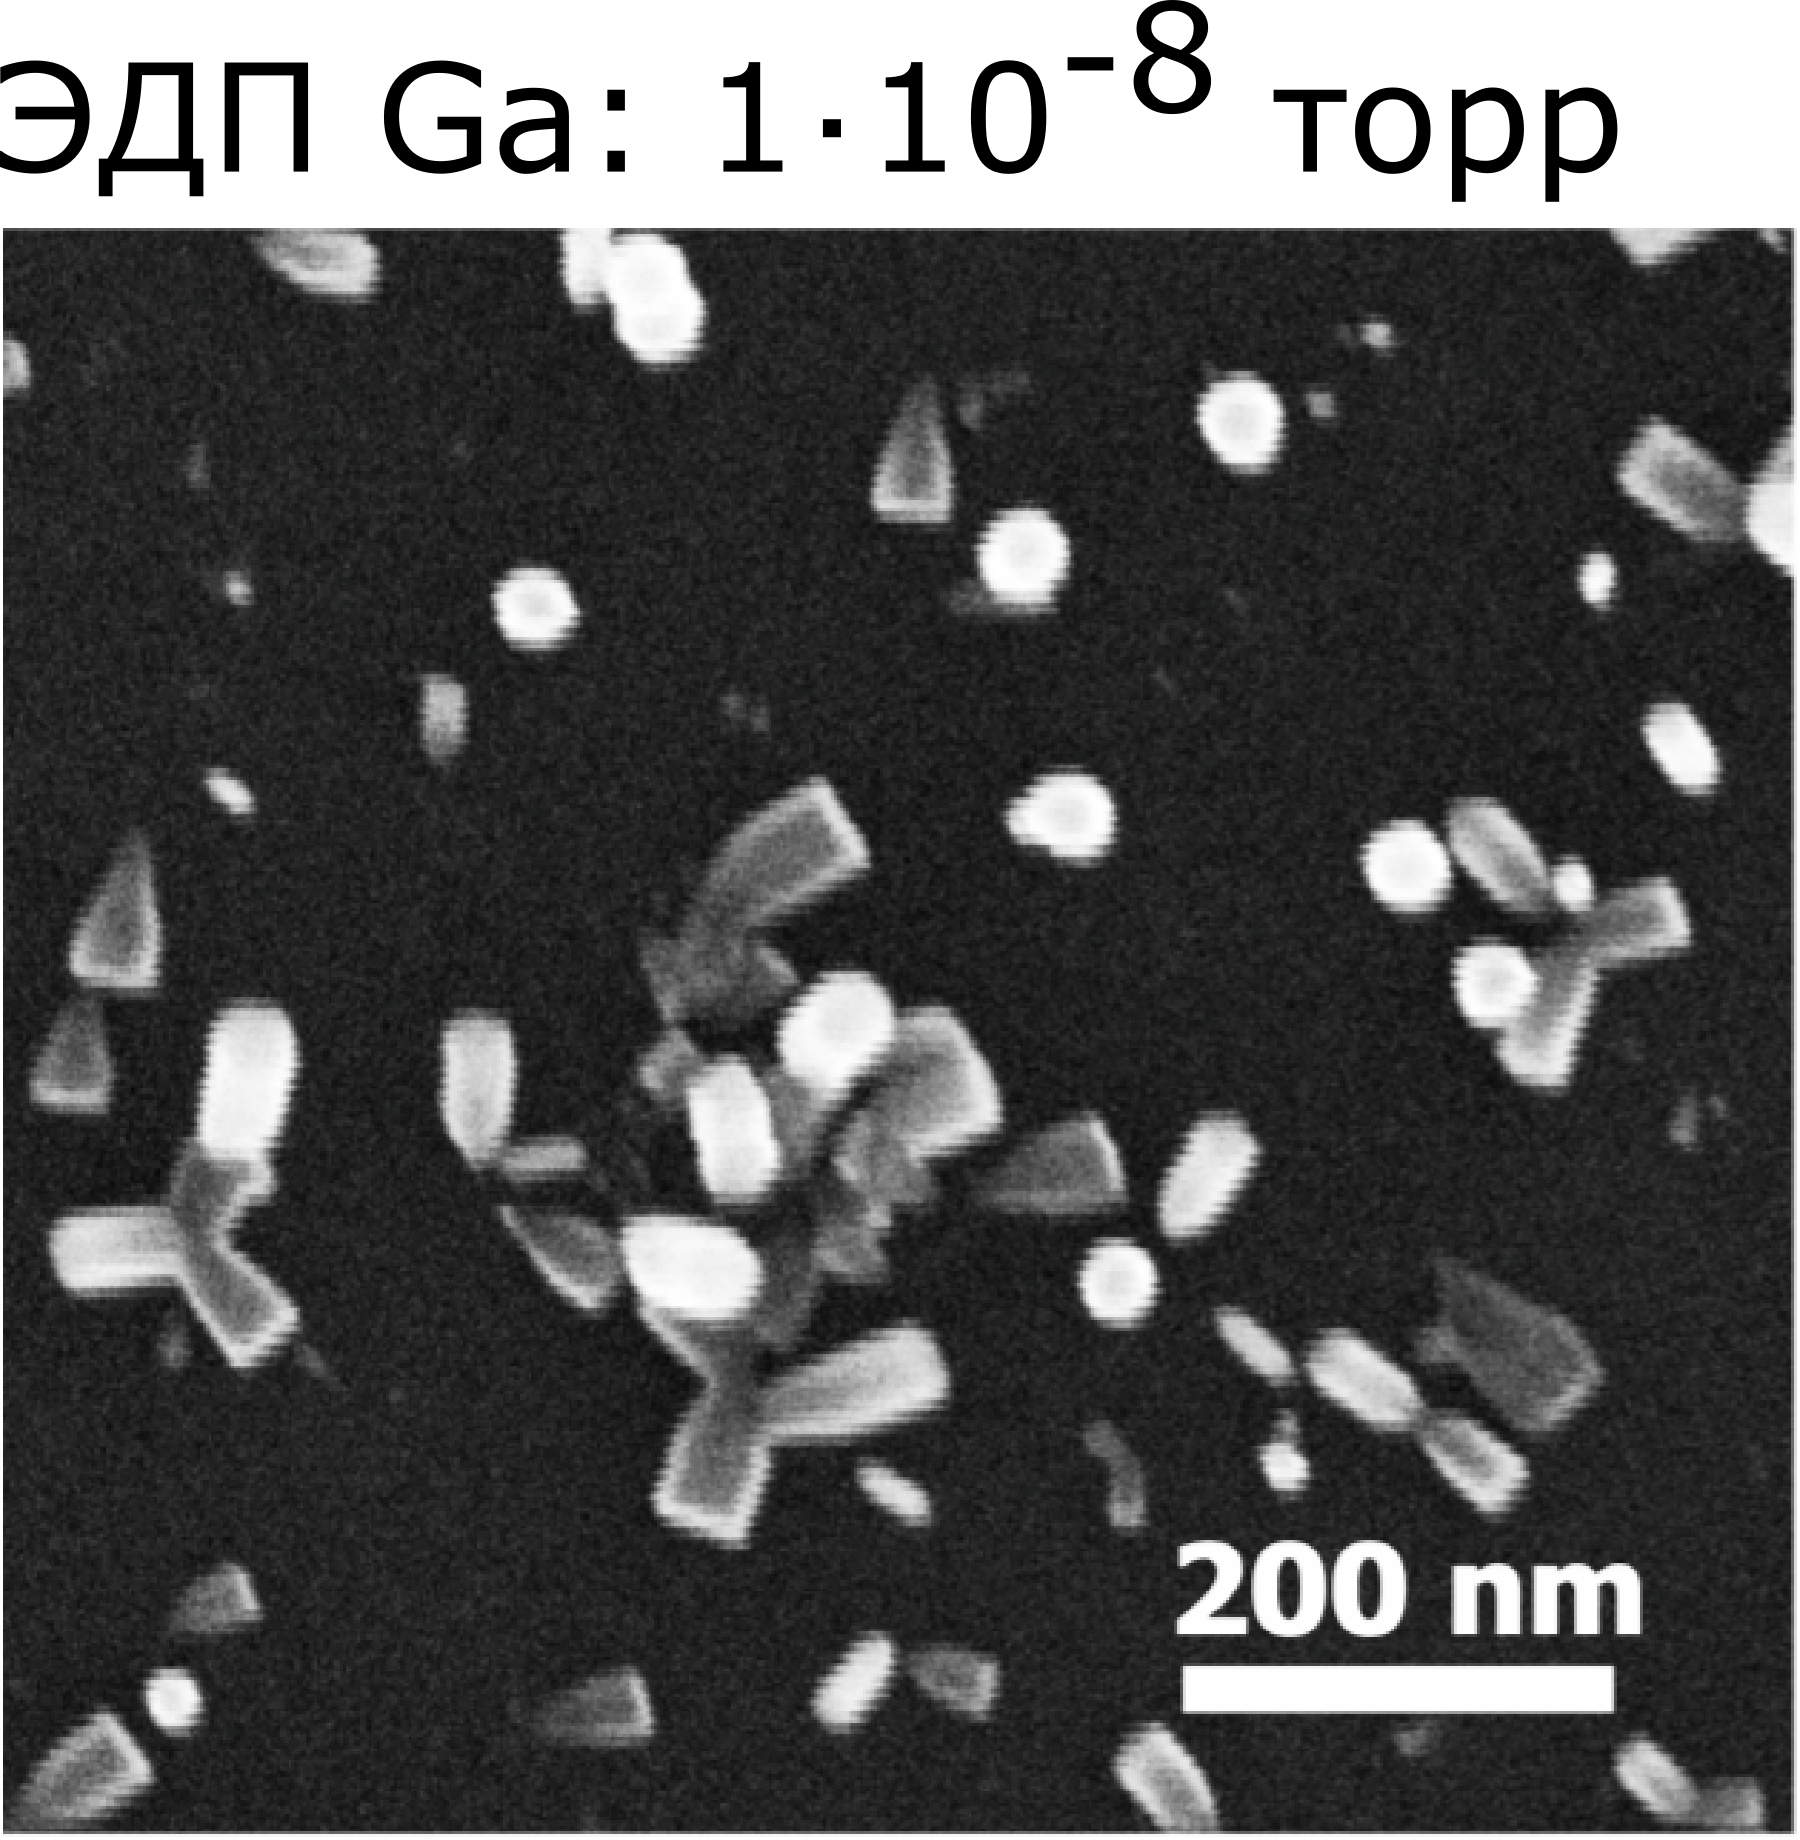
\includegraphics[width=0.25\linewidth]{Image_23_1}}
			\subcaptionbox{\label{fig:Image_23_2}}{%
				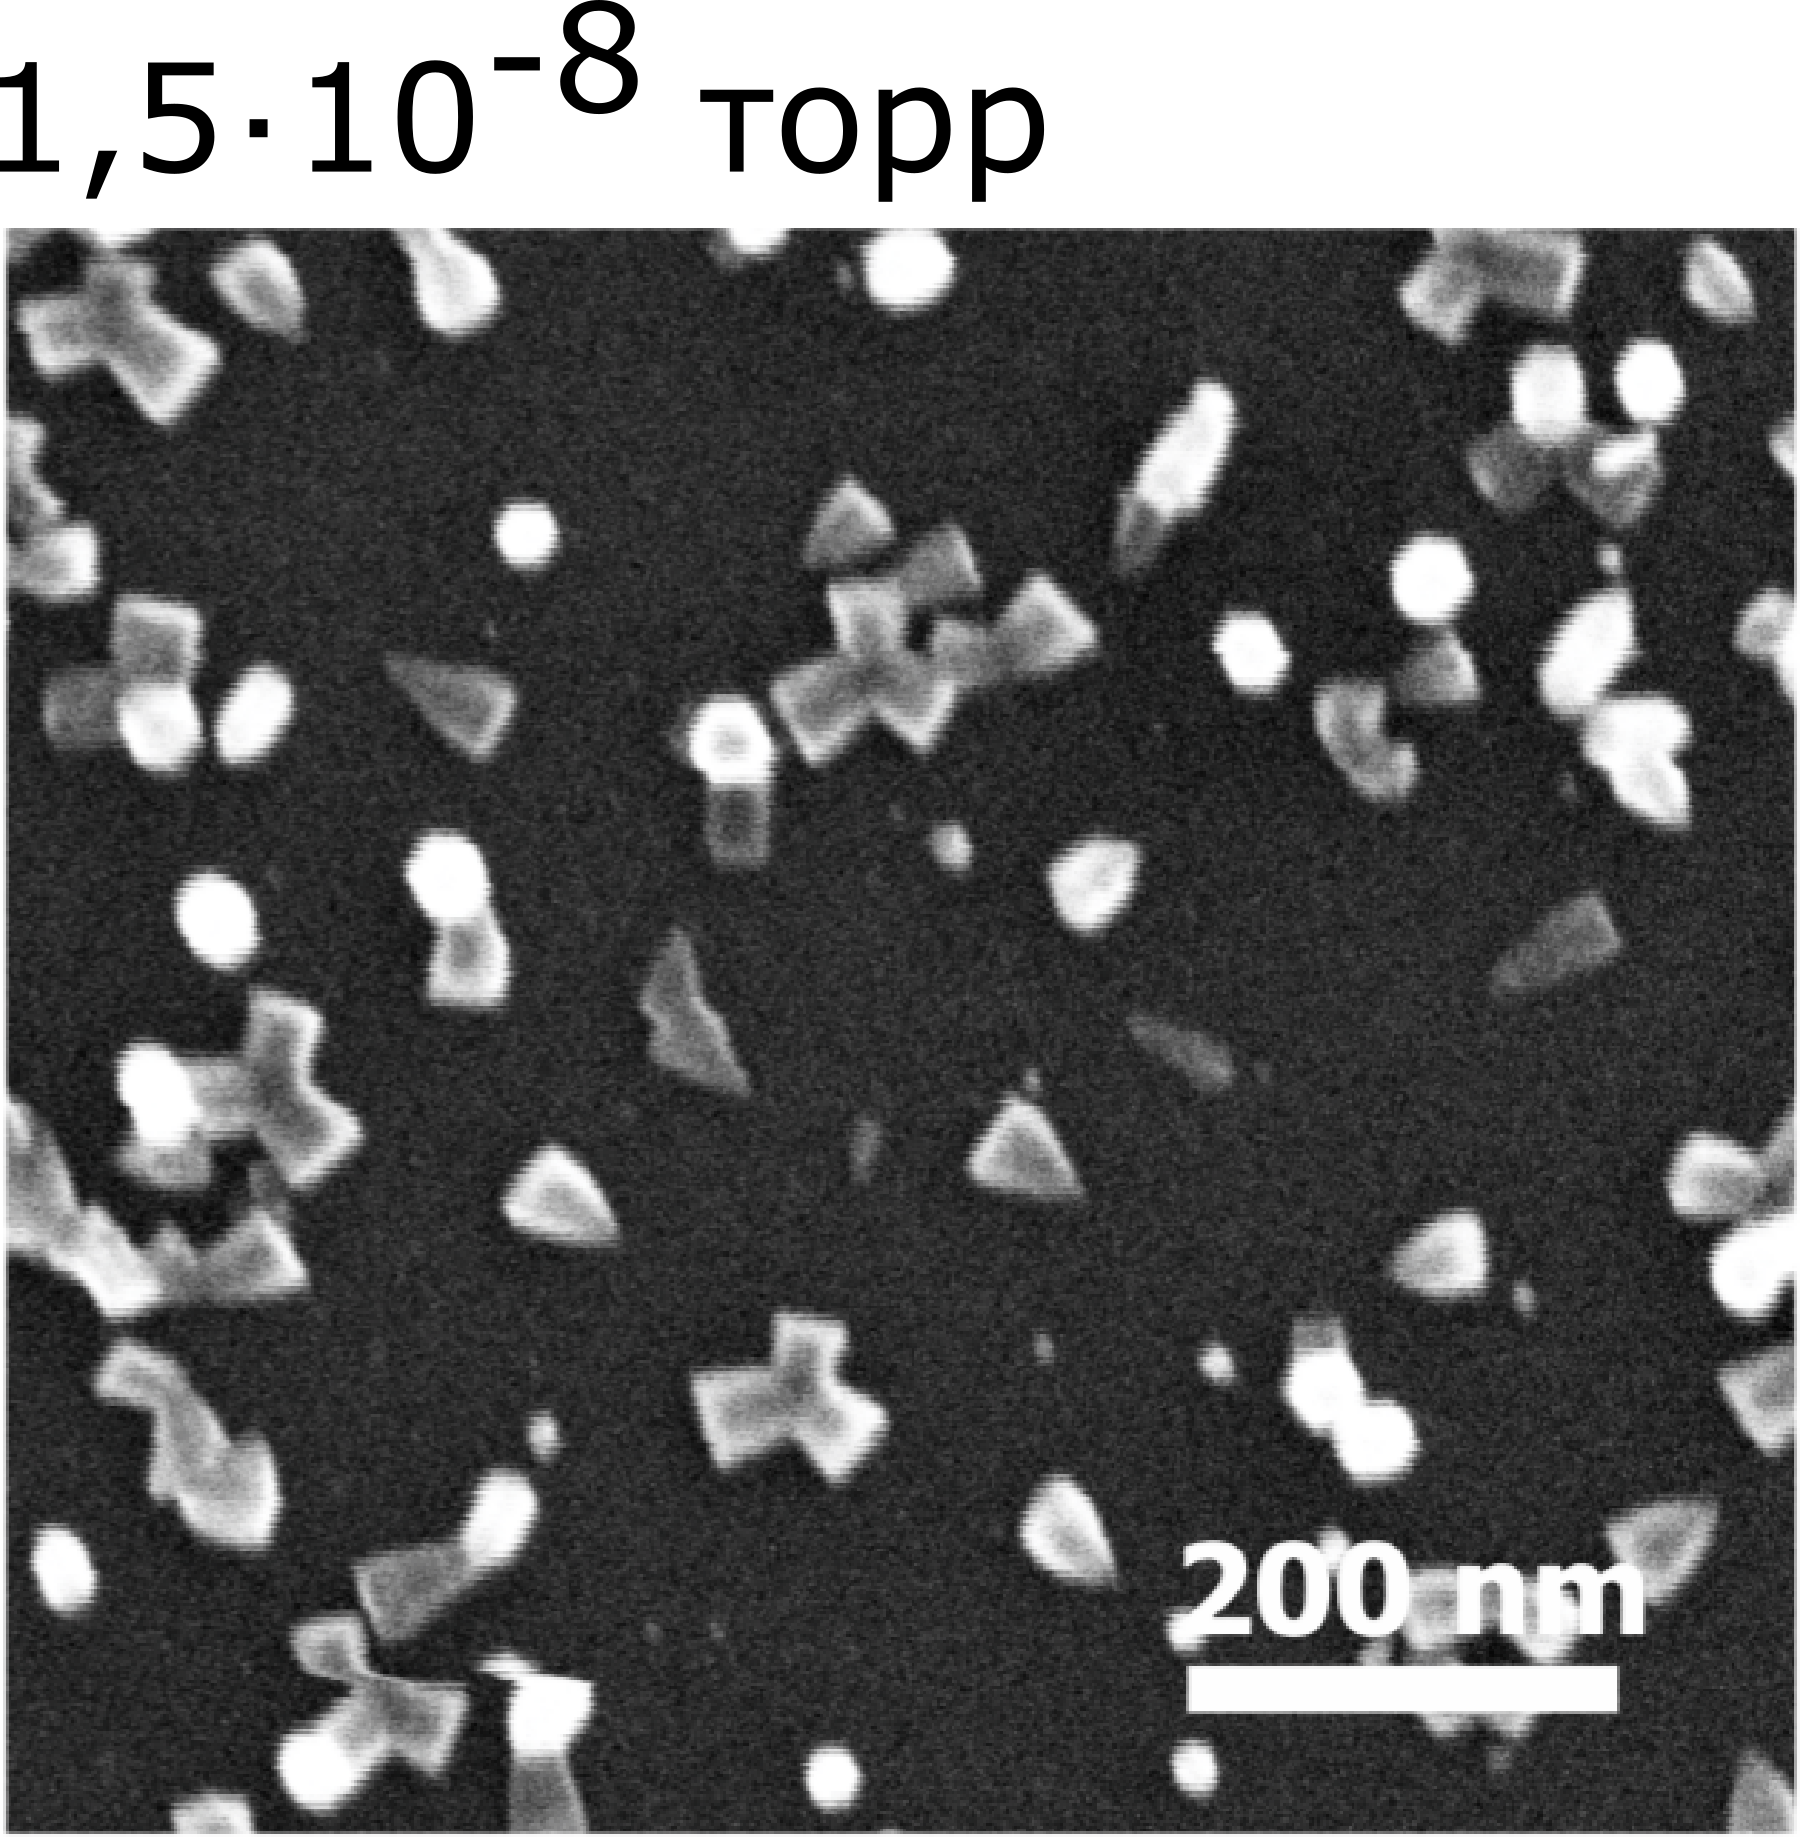
\includegraphics[width=0.25\linewidth]{Image_23_2}}
				\subcaptionbox{\label{fig:Image_23_3}}{%
				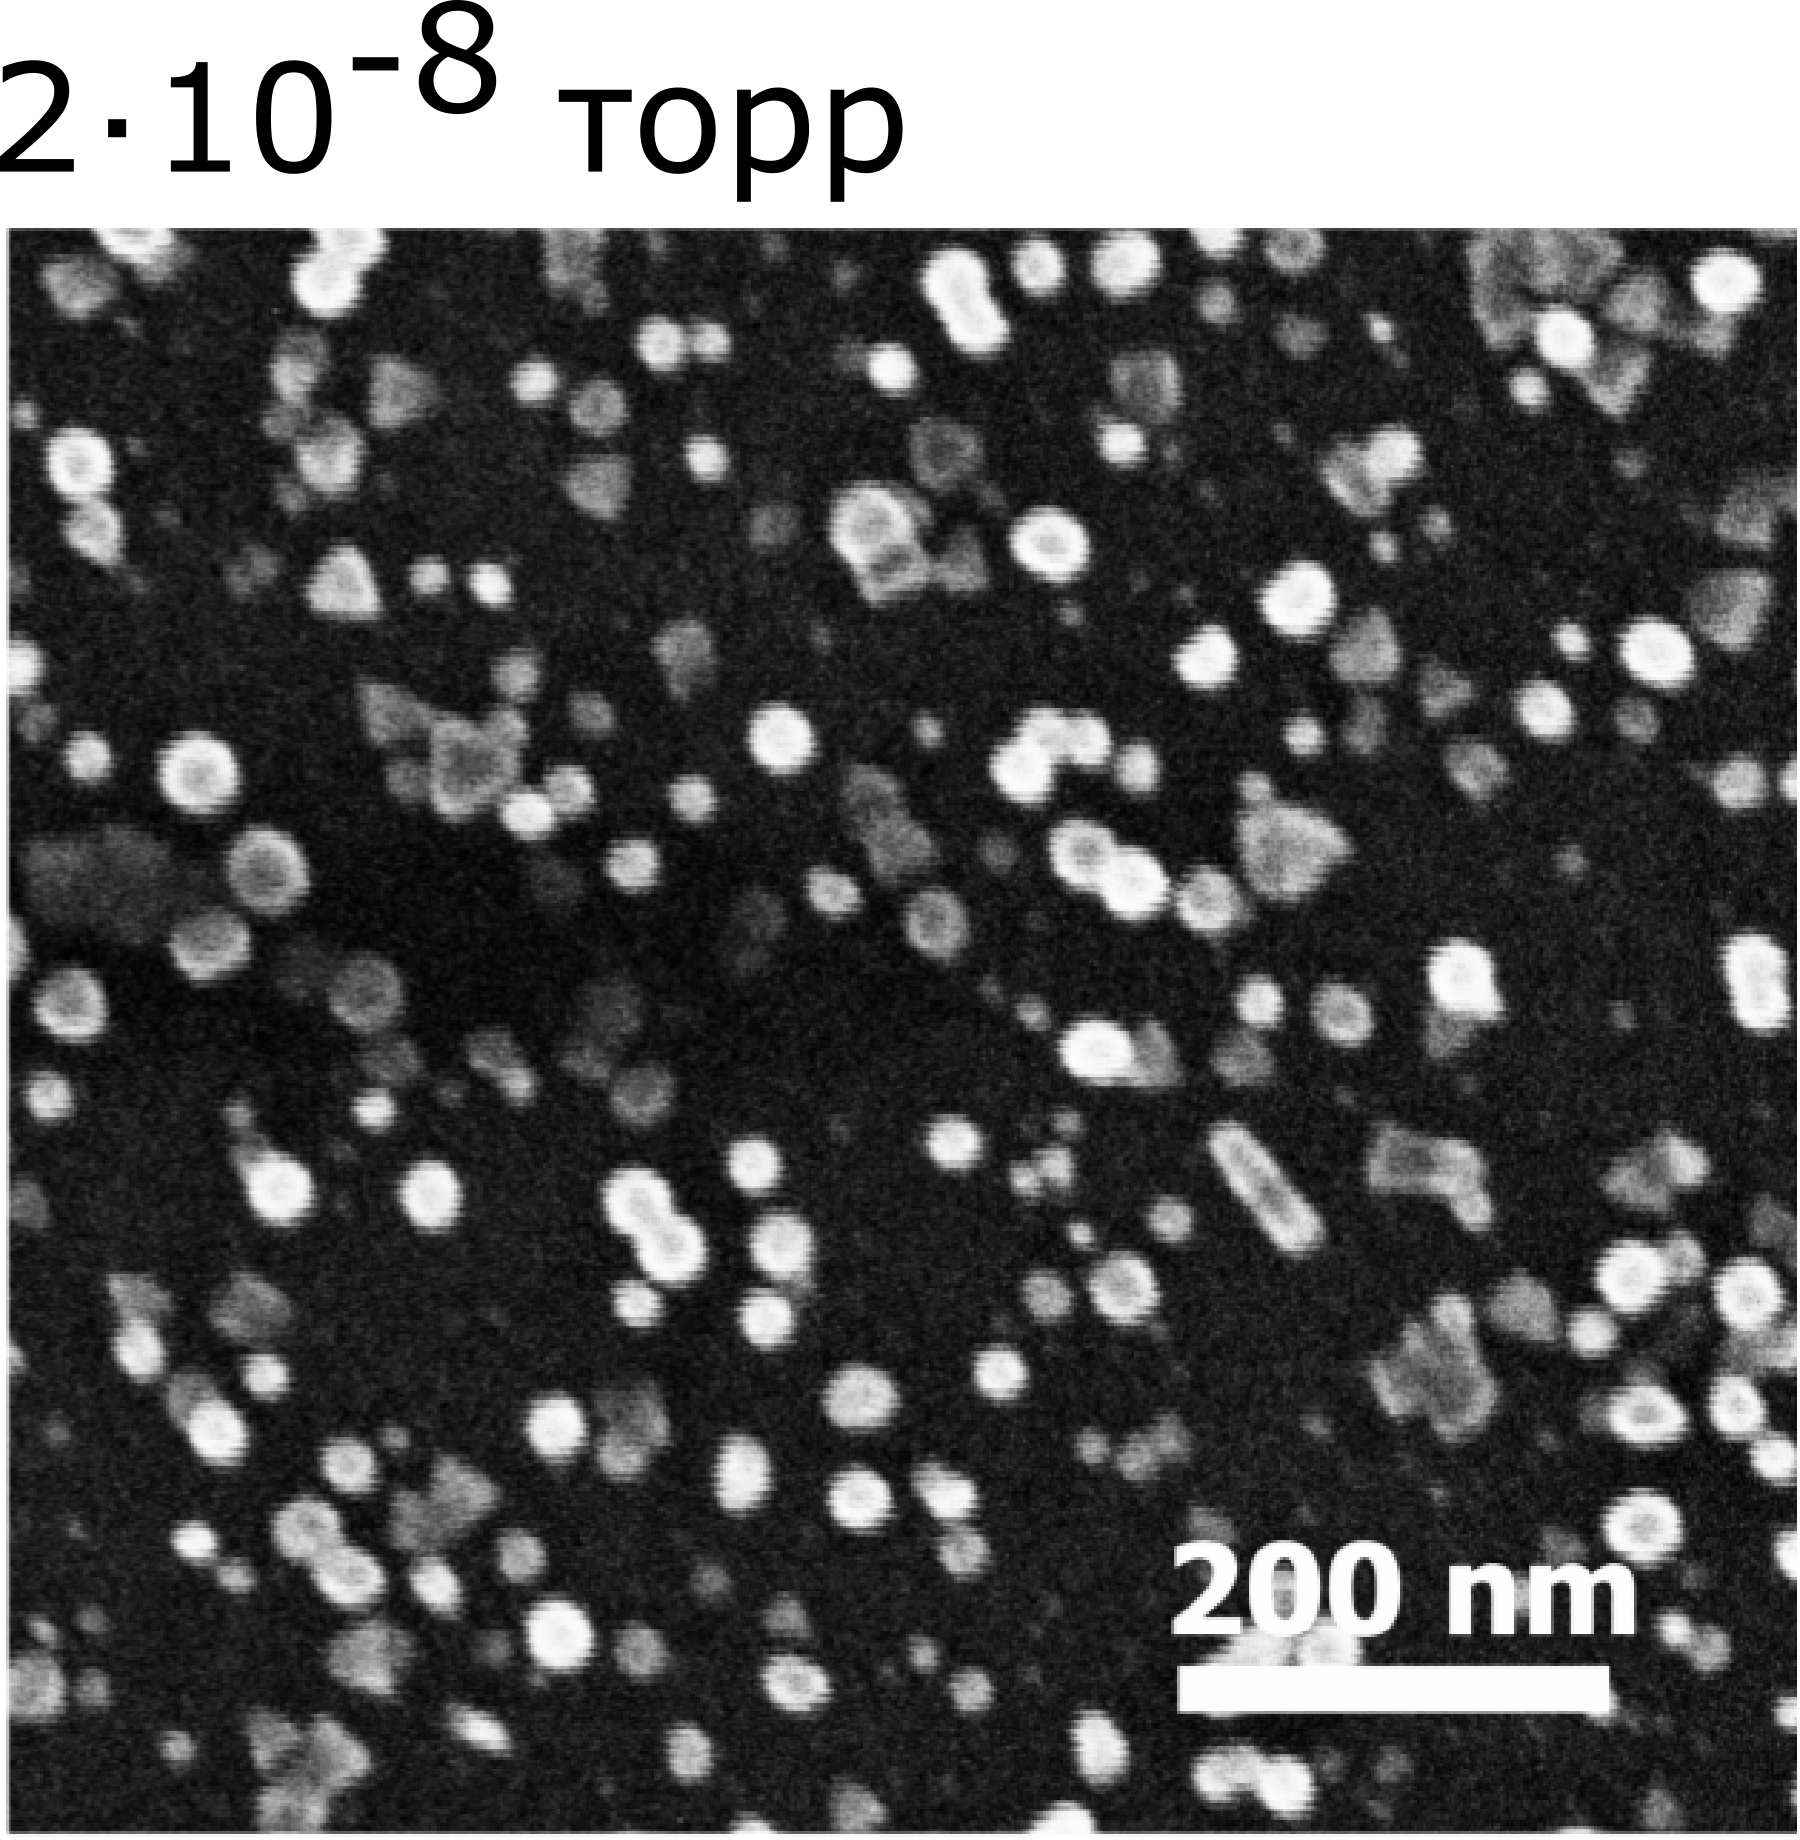
\includegraphics[width=0.25\linewidth]{Image_23_3}} } \legend{ЭДП Ga
				\(1 \cdot 10^{-8}\)~(а), \(1,5 \cdot 10^{-8}\)~(б), \(2 \cdot
				10^{-8}\)~\si{\torr}~(в)} \caption{РЭМ изображения наноструктур GaN,
		выращенных при различных ЭДП Ga}\label{fig:Image_23} \end{figure}

Согласно работе \cite{Voulot1998}, расход азота или ВЧ мощность влияет не
только на ЭДП активированного азота, но и на соотношение в нем атомов, молекул
и ионов \cite{Blant2000}, поэтому корреляции между расходом азота и потоком
активированного азота нелинейная. По этой причине параметры источника плазмы
сохранялись постоянными (расход азота 1~\si{\centi\meter^3\per\minute}, ВЧ
мощность 500~\si{\watt}).

Увеличение ЭДП Ga в исследуемом диапазоне уменьшает скорость роста вертикальных
и наклонённых ННК, снижает аспектное отношение ННК и триподов (длина/толщина)
(см.~рис.~\cref{fig:Image_24_1},~ \cref{fig:Image_24_2}), повышает сужение ННК
у основания. Поверхность подложки в основном занята триподами при ЭДП Ga \(1,5
\cdot 10^{-8}\)~\si{\torr}, а при потоке выше и ниже этого значения на
поверхности доминируют ННК (см.~рис.~\cref{fig:Image_24_1}).

\begin{figure}[ht] \centerfloat{ \subcaptionbox{\label{fig:Image_24_1_1}}{%
			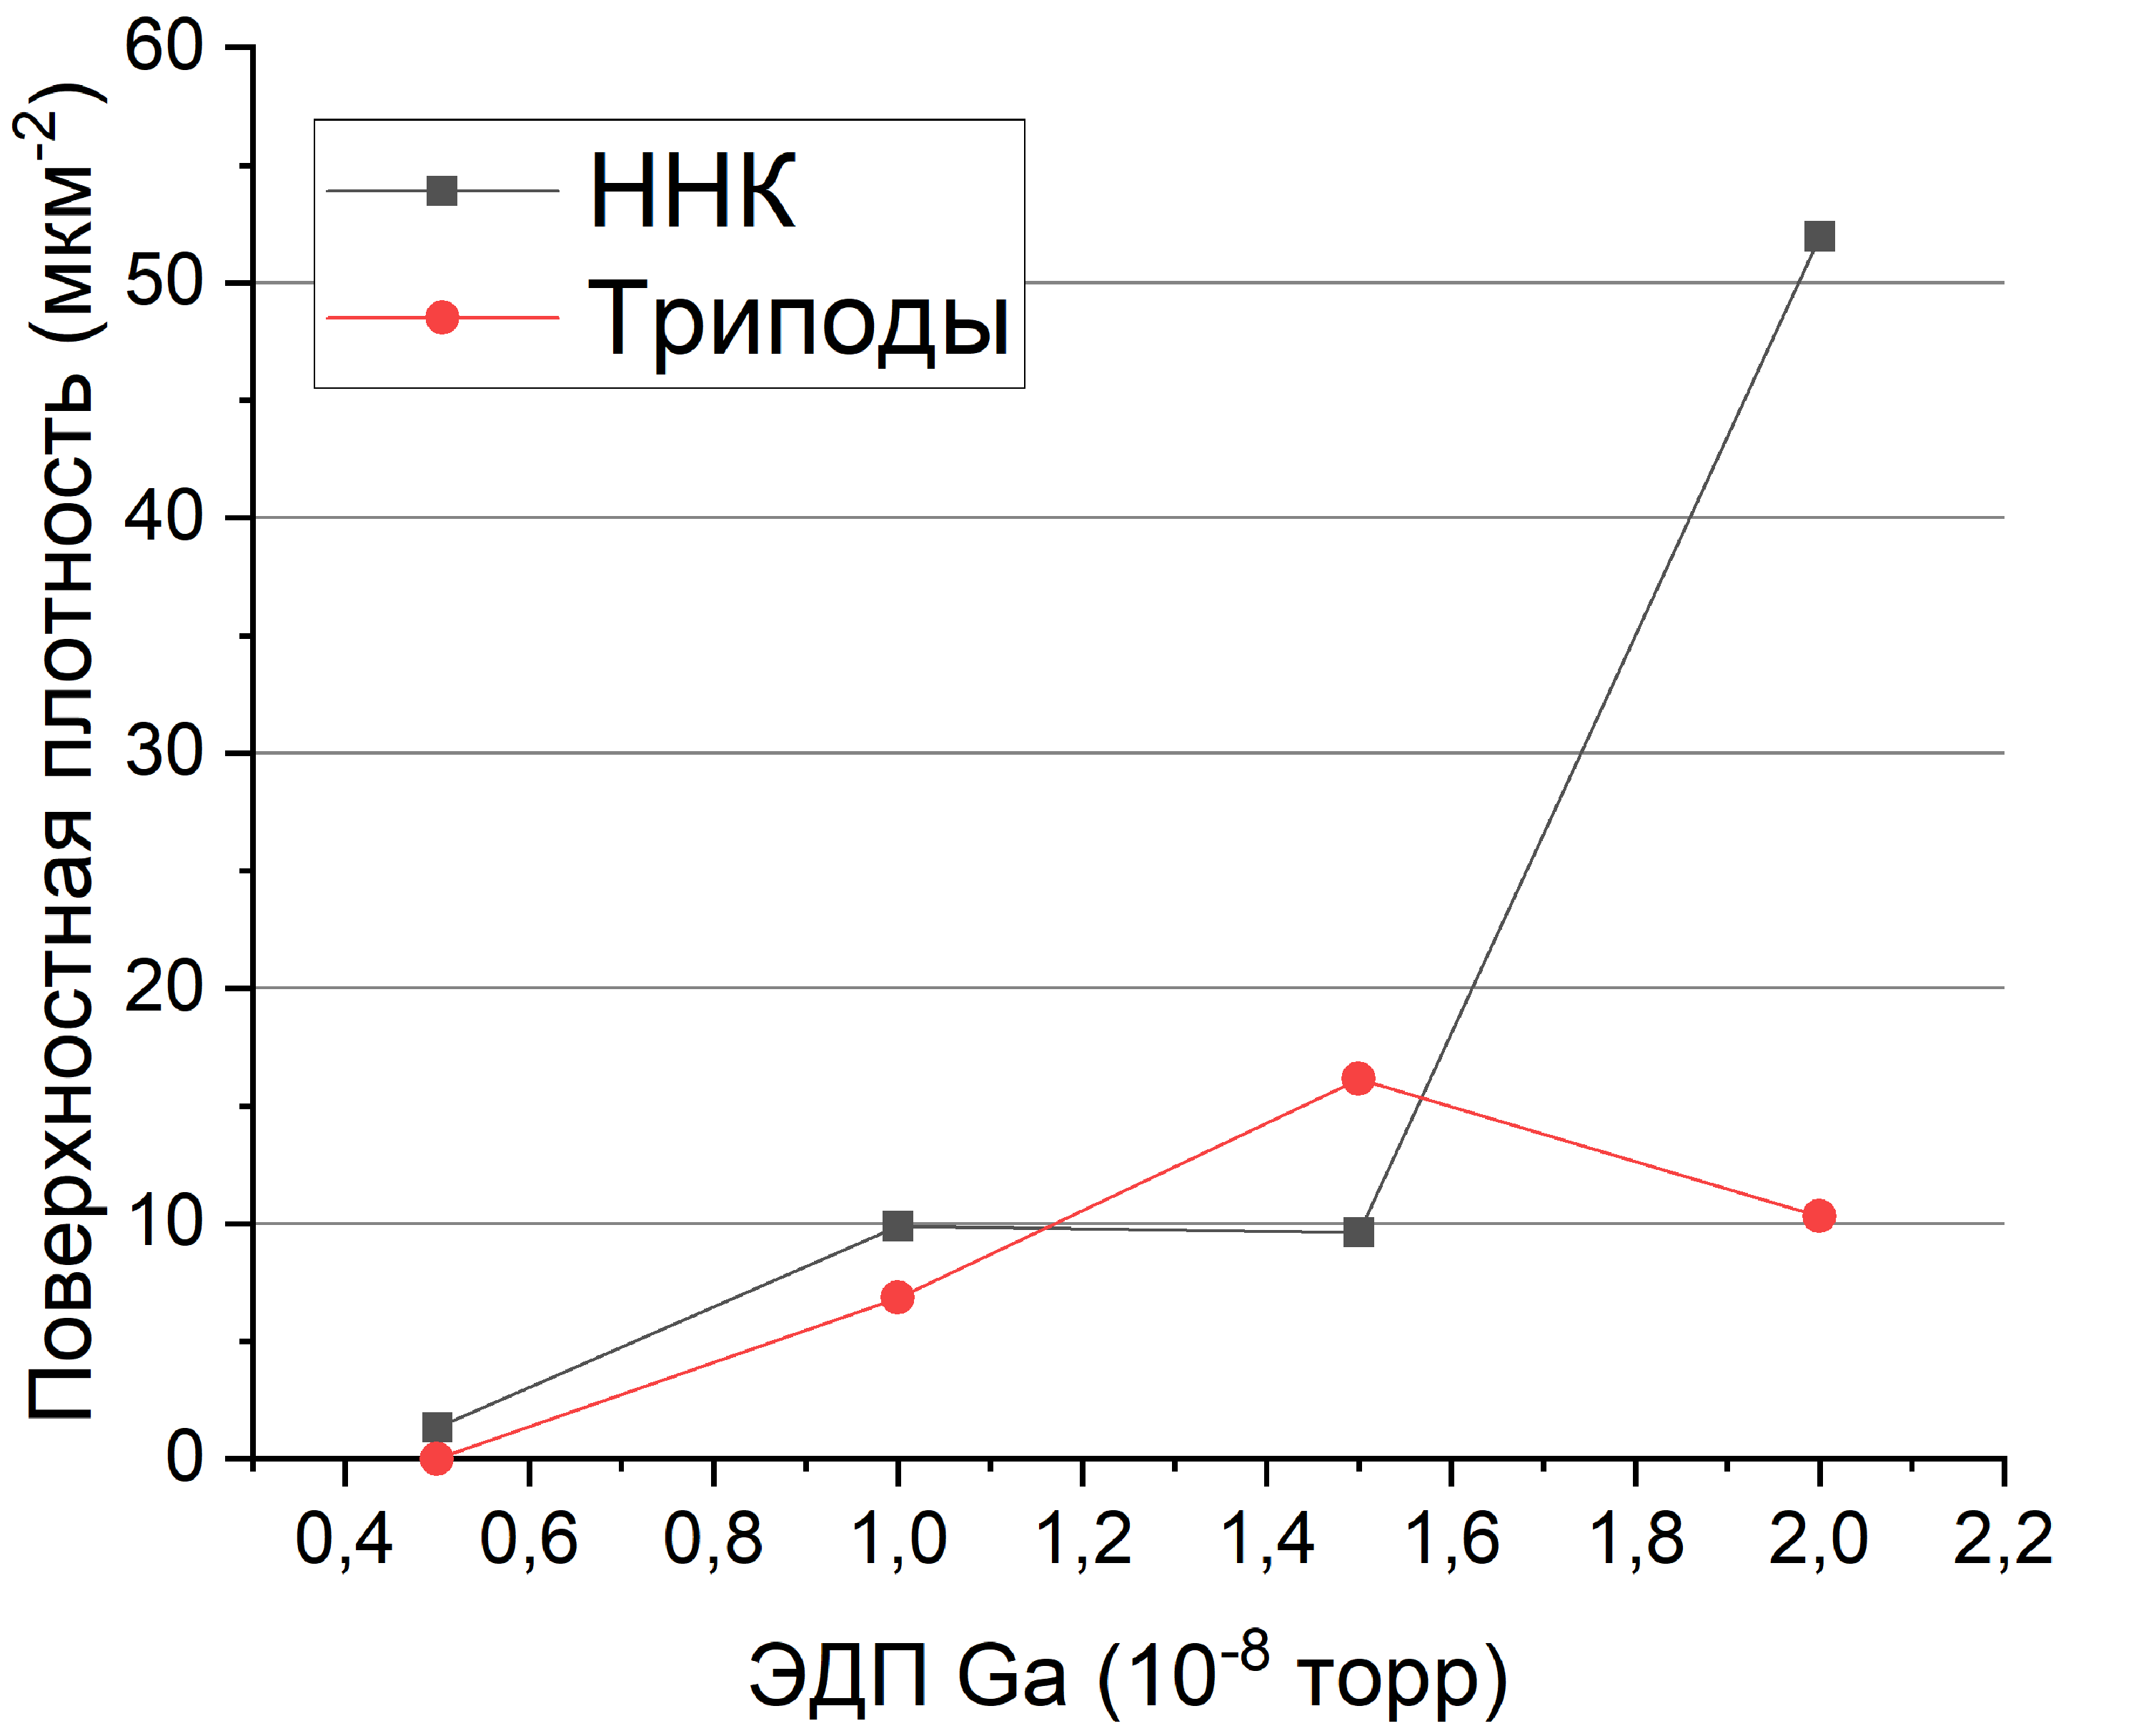
\includegraphics[width=0.48\linewidth]{Image_24_1_1}}
			\subcaptionbox{\label{fig:Image_24_1_2}}{%
			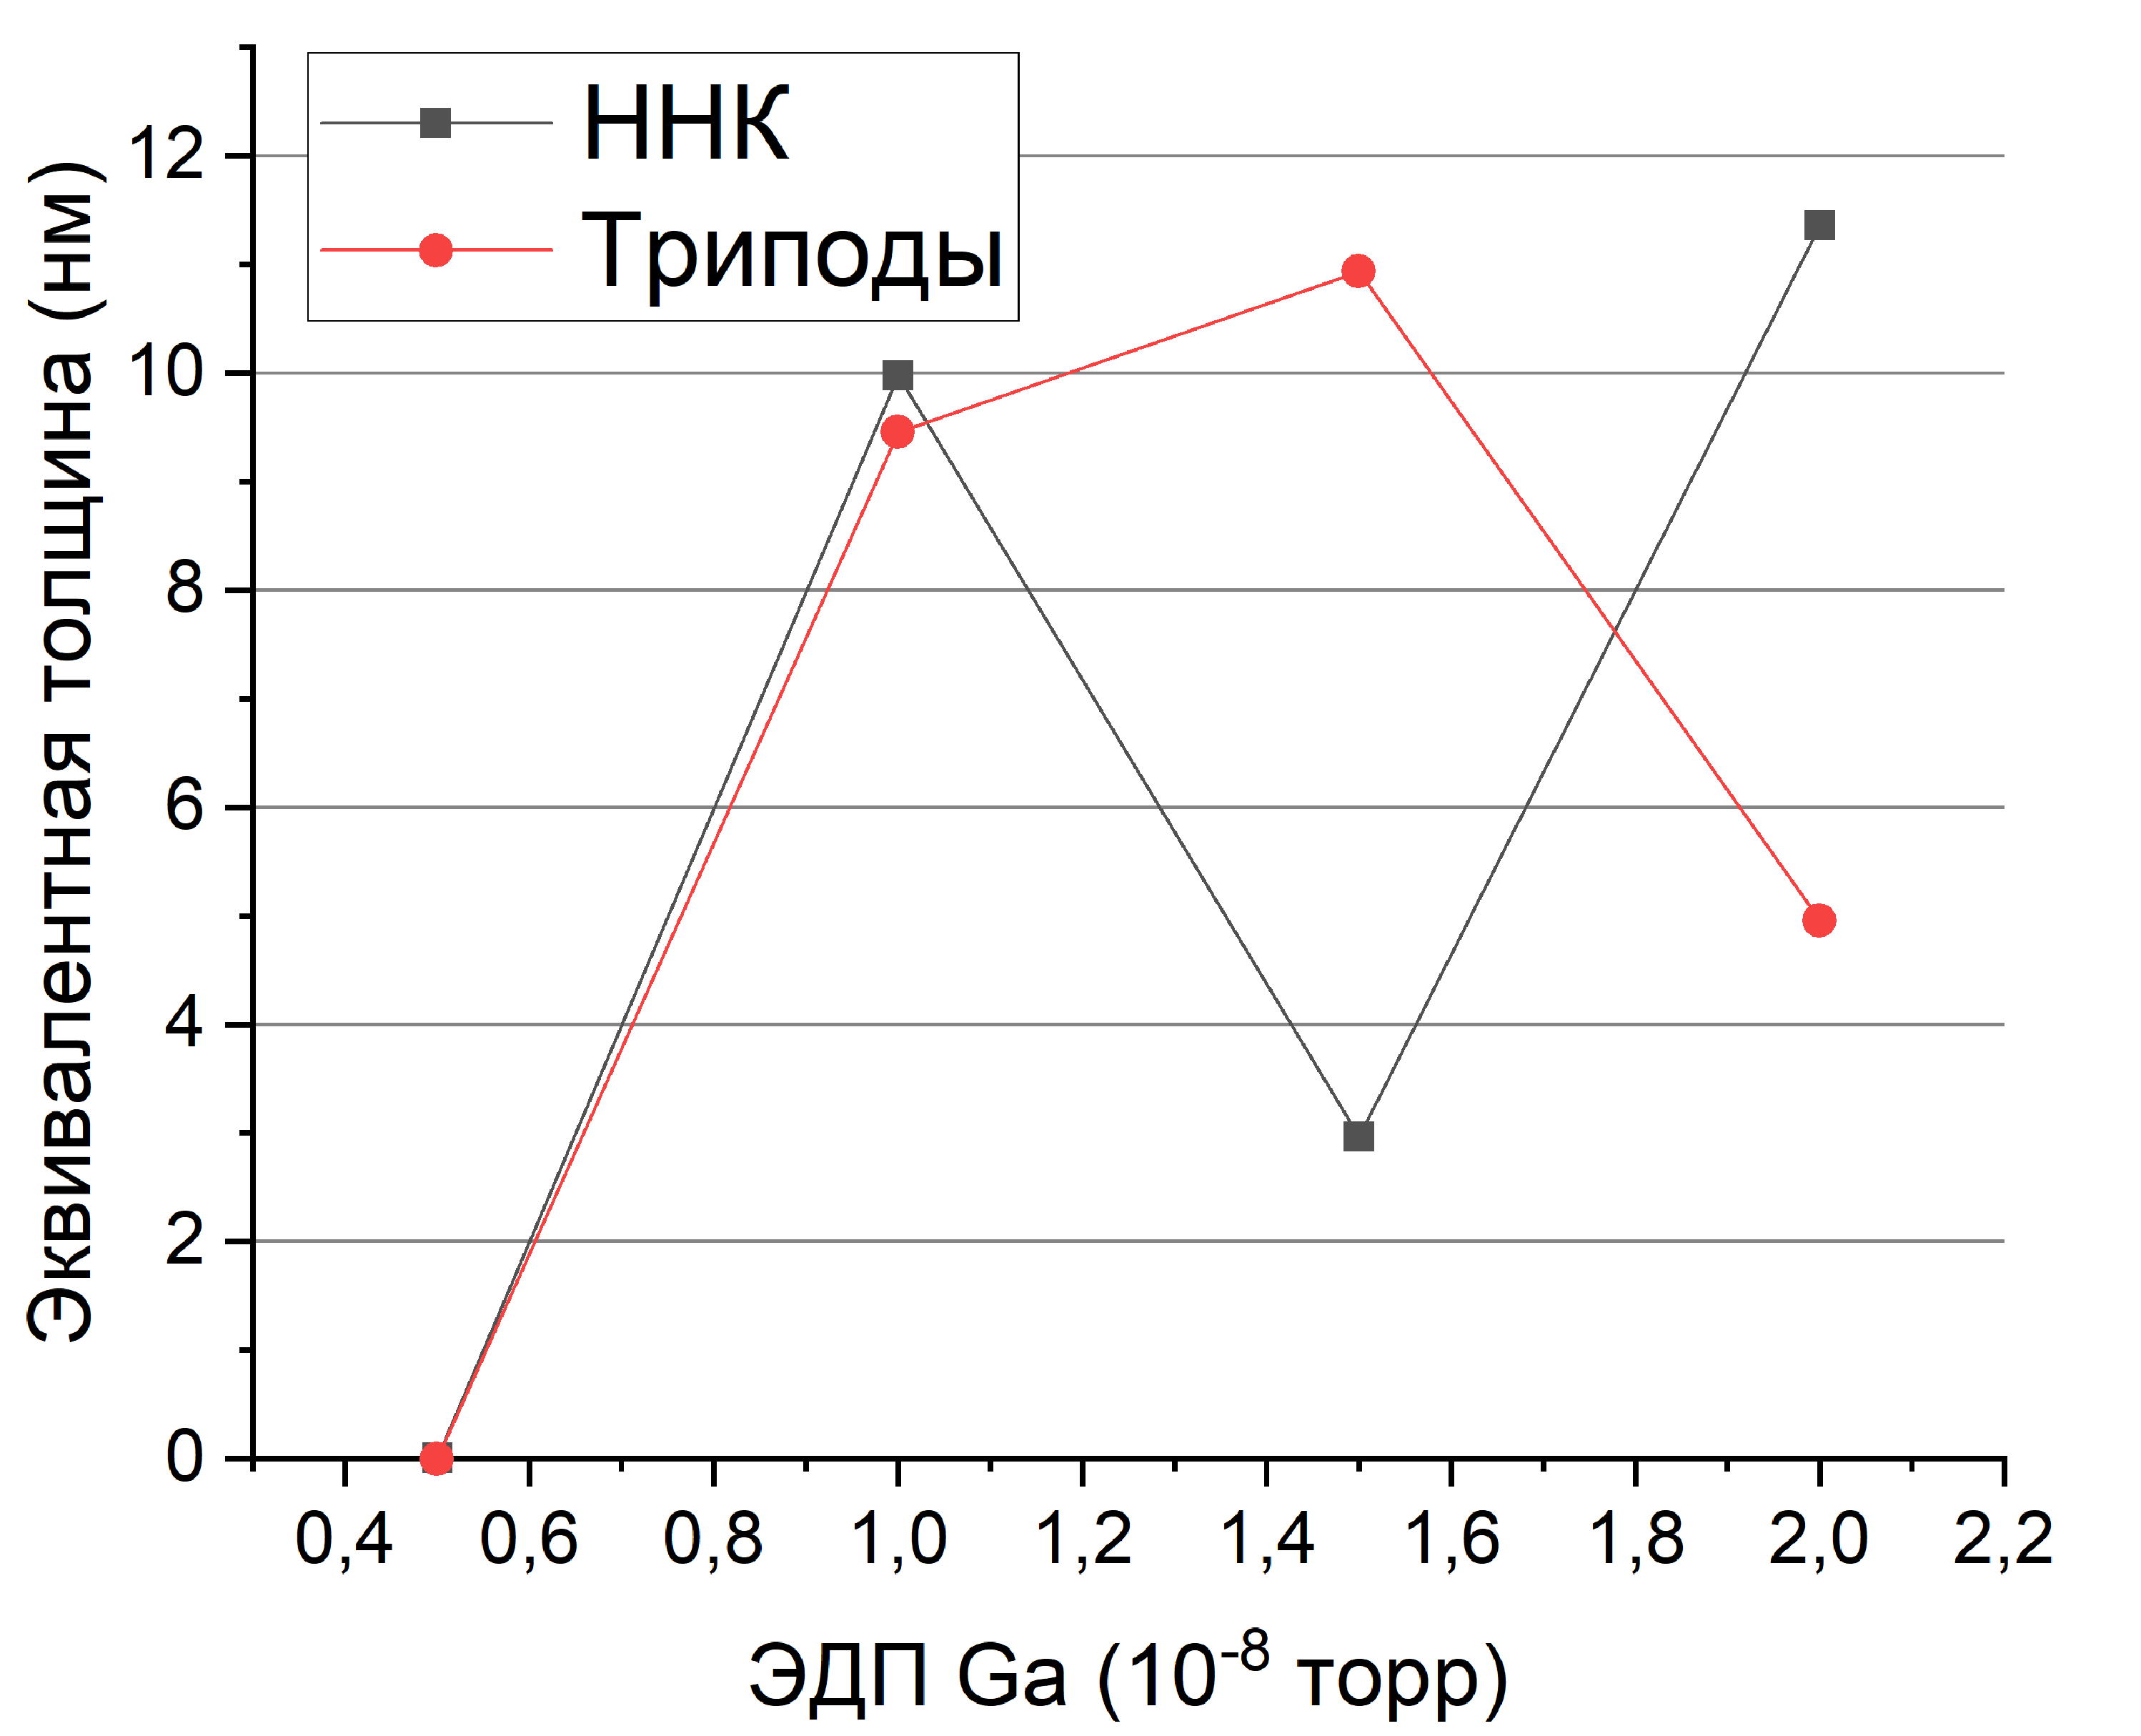
\includegraphics[width=0.48\linewidth]{Image_24_1_2}} }
			\caption{Зависимости поверхностной плотности~(а) и эквивалентной толщины
			осаждённого материала~(б) наноструктур GaN от ЭДП
		Ga}\label{fig:Image_24_1} \end{figure}

\begin{figure}[ht] \centerfloat{
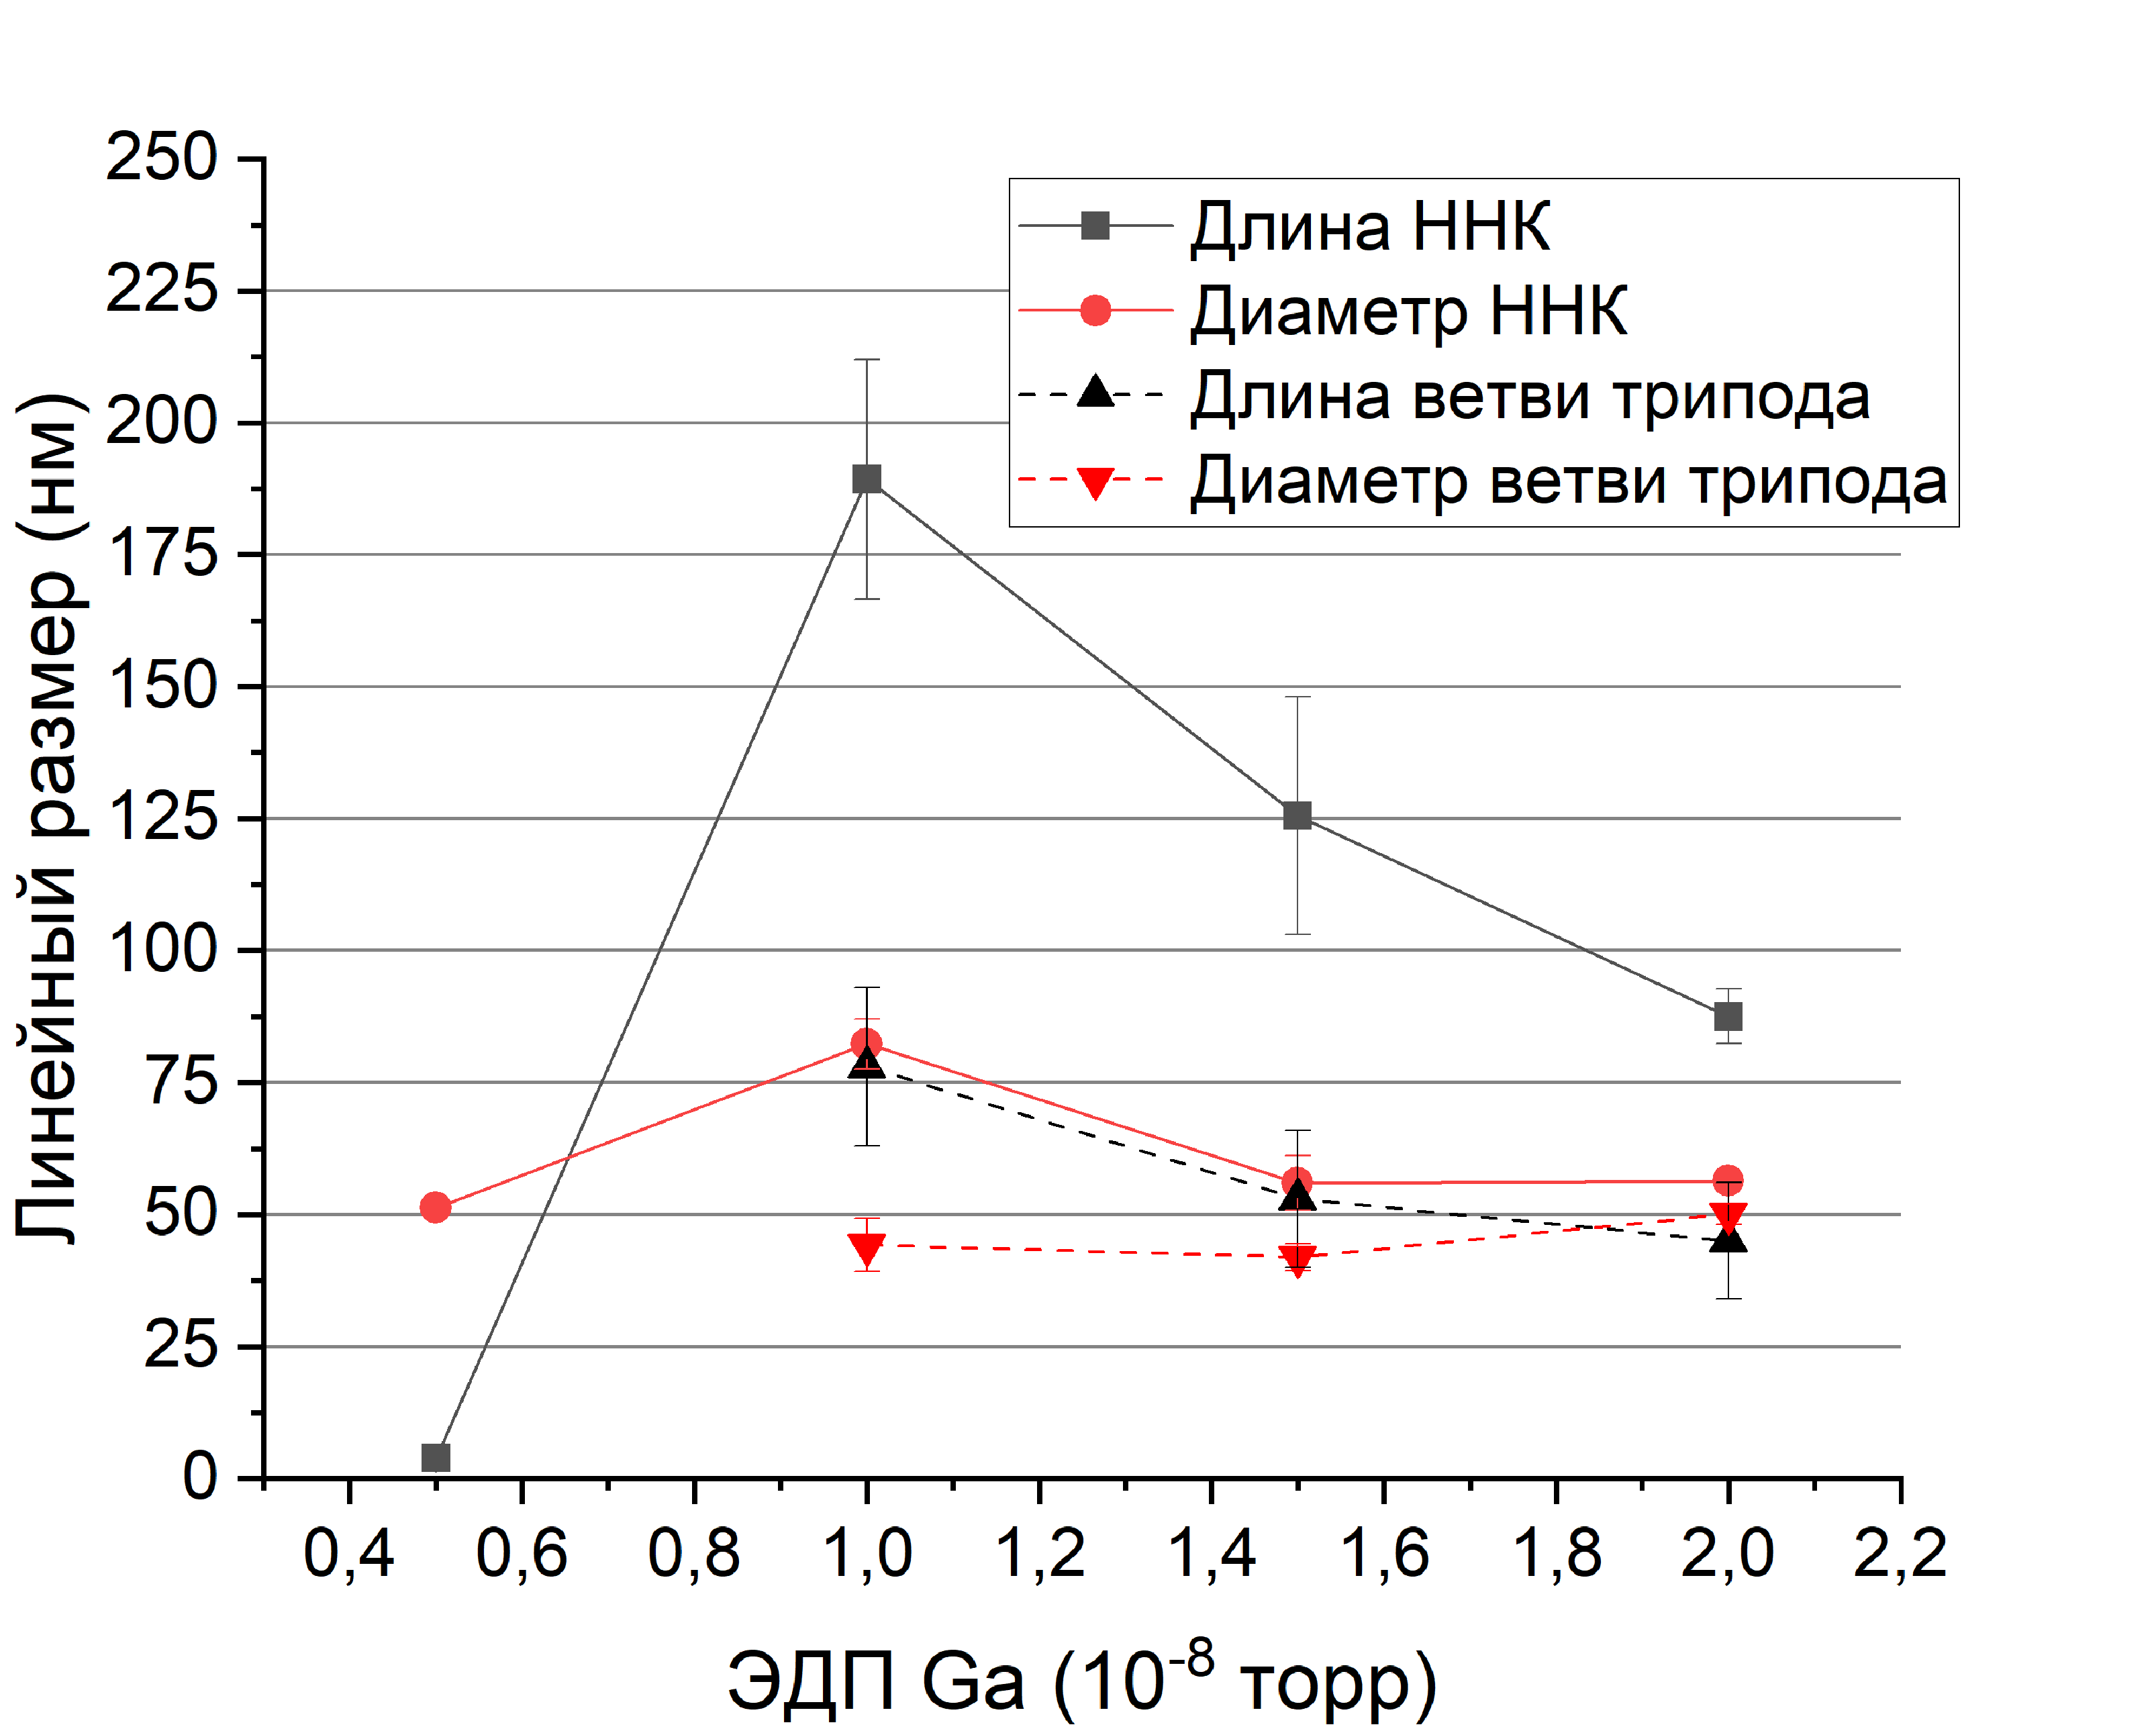
\includegraphics[width=0.6\linewidth]{Image_24_2} } \caption{Зависимости
линейных размеров наноструктур GaN от ЭДП Ga}\label{fig:Image_24_2}
\end{figure}

Эквивалентная толщина осаждаемого материала (см.~рис.~\cref{fig:Image_24_1_2})
не пропорциональна ЭДП Ga~--- увеличение поверхностной плотности
(см.~рис.~\cref{fig:Image_24_1_1}) компенсируется уменьшением среднего
поперечного размера наноструктур (см.~рис.~\cref{fig:Image_24_2}).

Исследуемые наноструктуры формировались в узком температурном диапазоне с 690 до
710~\si{\degreeCelsius} (см.~рис.~\cref{fig:Image_25}). При температуре роста
690~\si{\degreeCelsius} поверхностная плотность триподов становится настолько
высокой, что они срастаются и покрывают почти всю поверхность подложки
(см.~рис.~\cref{fig:Image_26_1_1}). Поверхностная плотность наноструктур быстро
падает с температурой. Формирование триподов полностью подавляется при
температурах выше 705~\si{\degreeCelsius}.

\begin{figure}[ht] \centerfloat{ \subcaptionbox{\label{fig:Image_25_1}}{%
			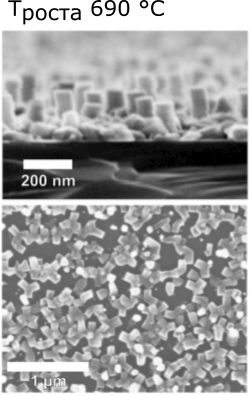
\includegraphics[width=0.25\linewidth]{Image_25_1}}
			\subcaptionbox{\label{fig:Image_25_2}}{%
				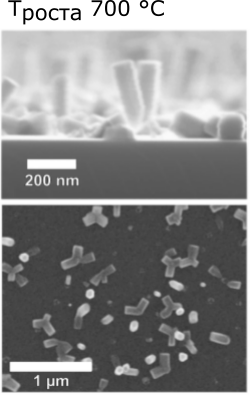
\includegraphics[width=0.25\linewidth]{Image_25_2}}
				\subcaptionbox{\label{fig:Image_25_3}}{%
				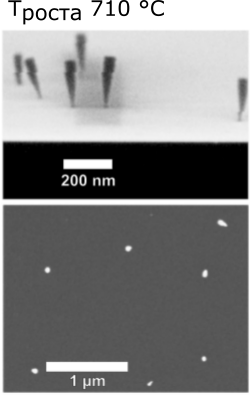
\includegraphics[width=0.25\linewidth]{Image_25_3}} } \legend{Ростовая
				температура: 690~\si{\degreeCelsius}~(а), 700~\si{\degreeCelsius}~(б),
				710~\si{\degreeCelsius}~(в)} \caption{РЭМ изображения (вид сверху и
				сбоку) морфологии наноструктур GaN, синтезированных при различных
		температурах подложки}\label{fig:Image_25} \end{figure}

\begin{figure}[ht] \centerfloat{ \subcaptionbox{\label{fig:Image_26_1_1}}{%
			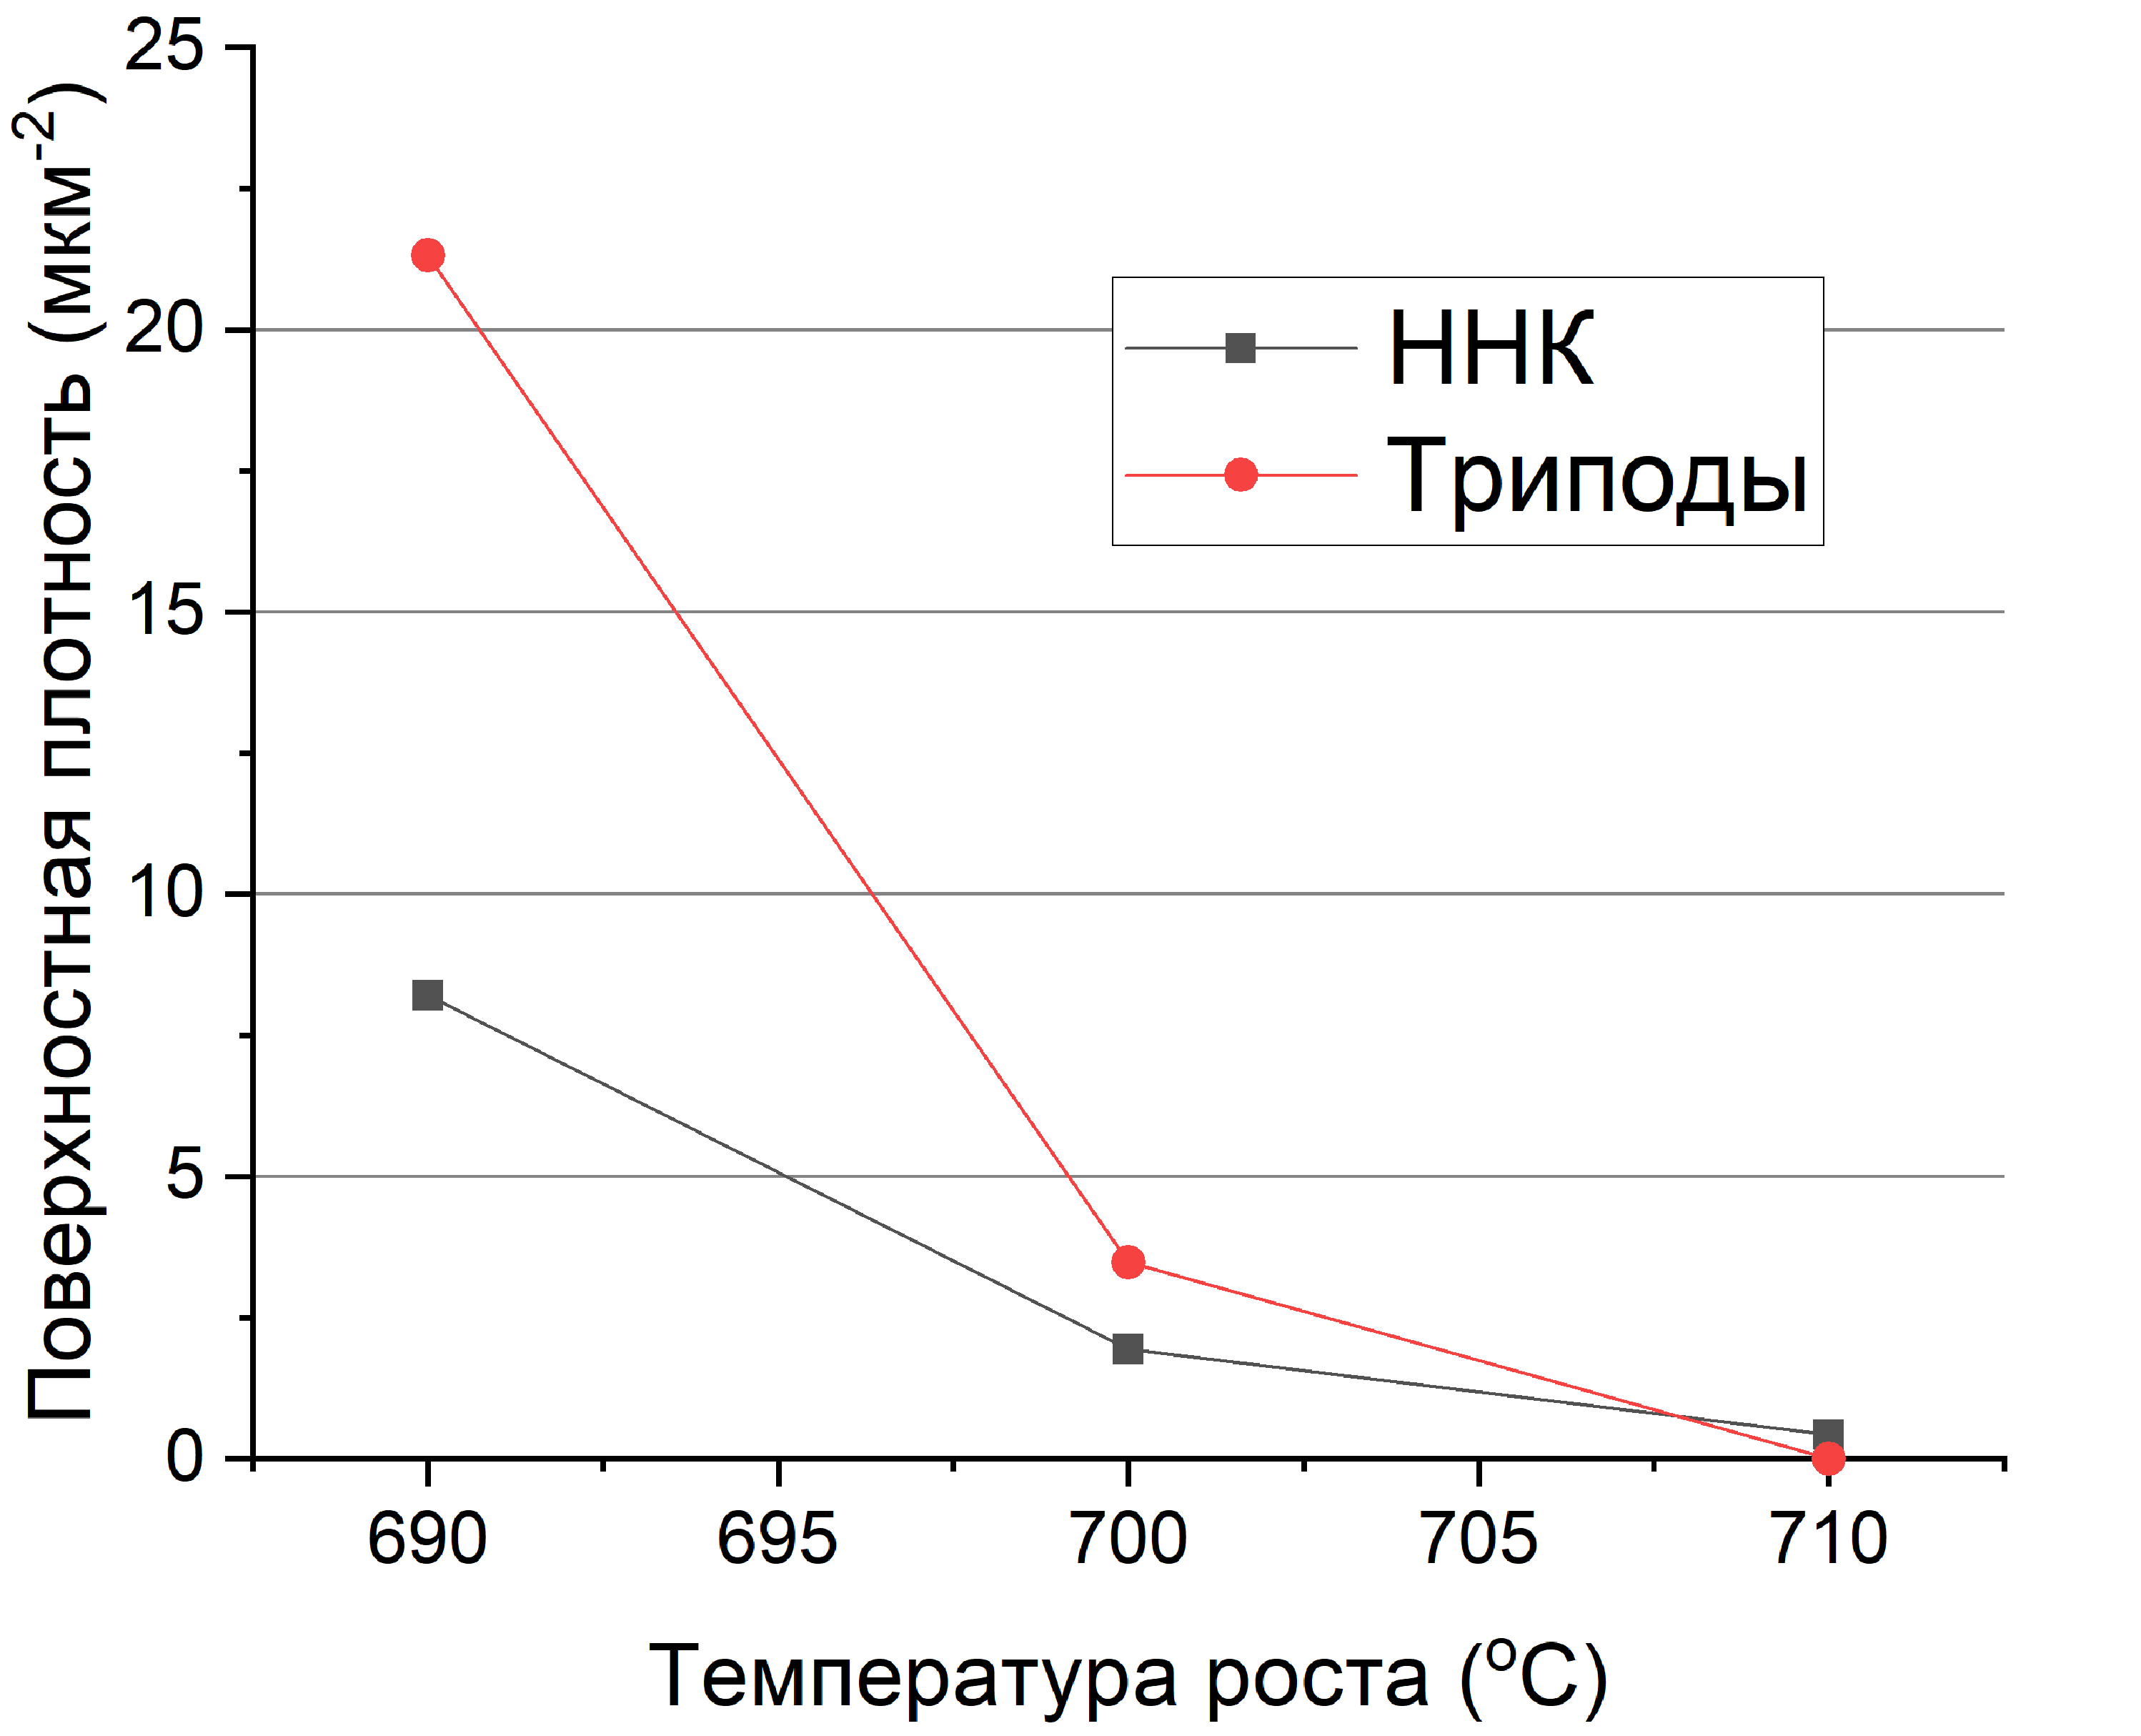
\includegraphics[width=0.48\linewidth]{Image_26_1_1}}
			\subcaptionbox{\label{fig:Image_26_1_2}}{%
			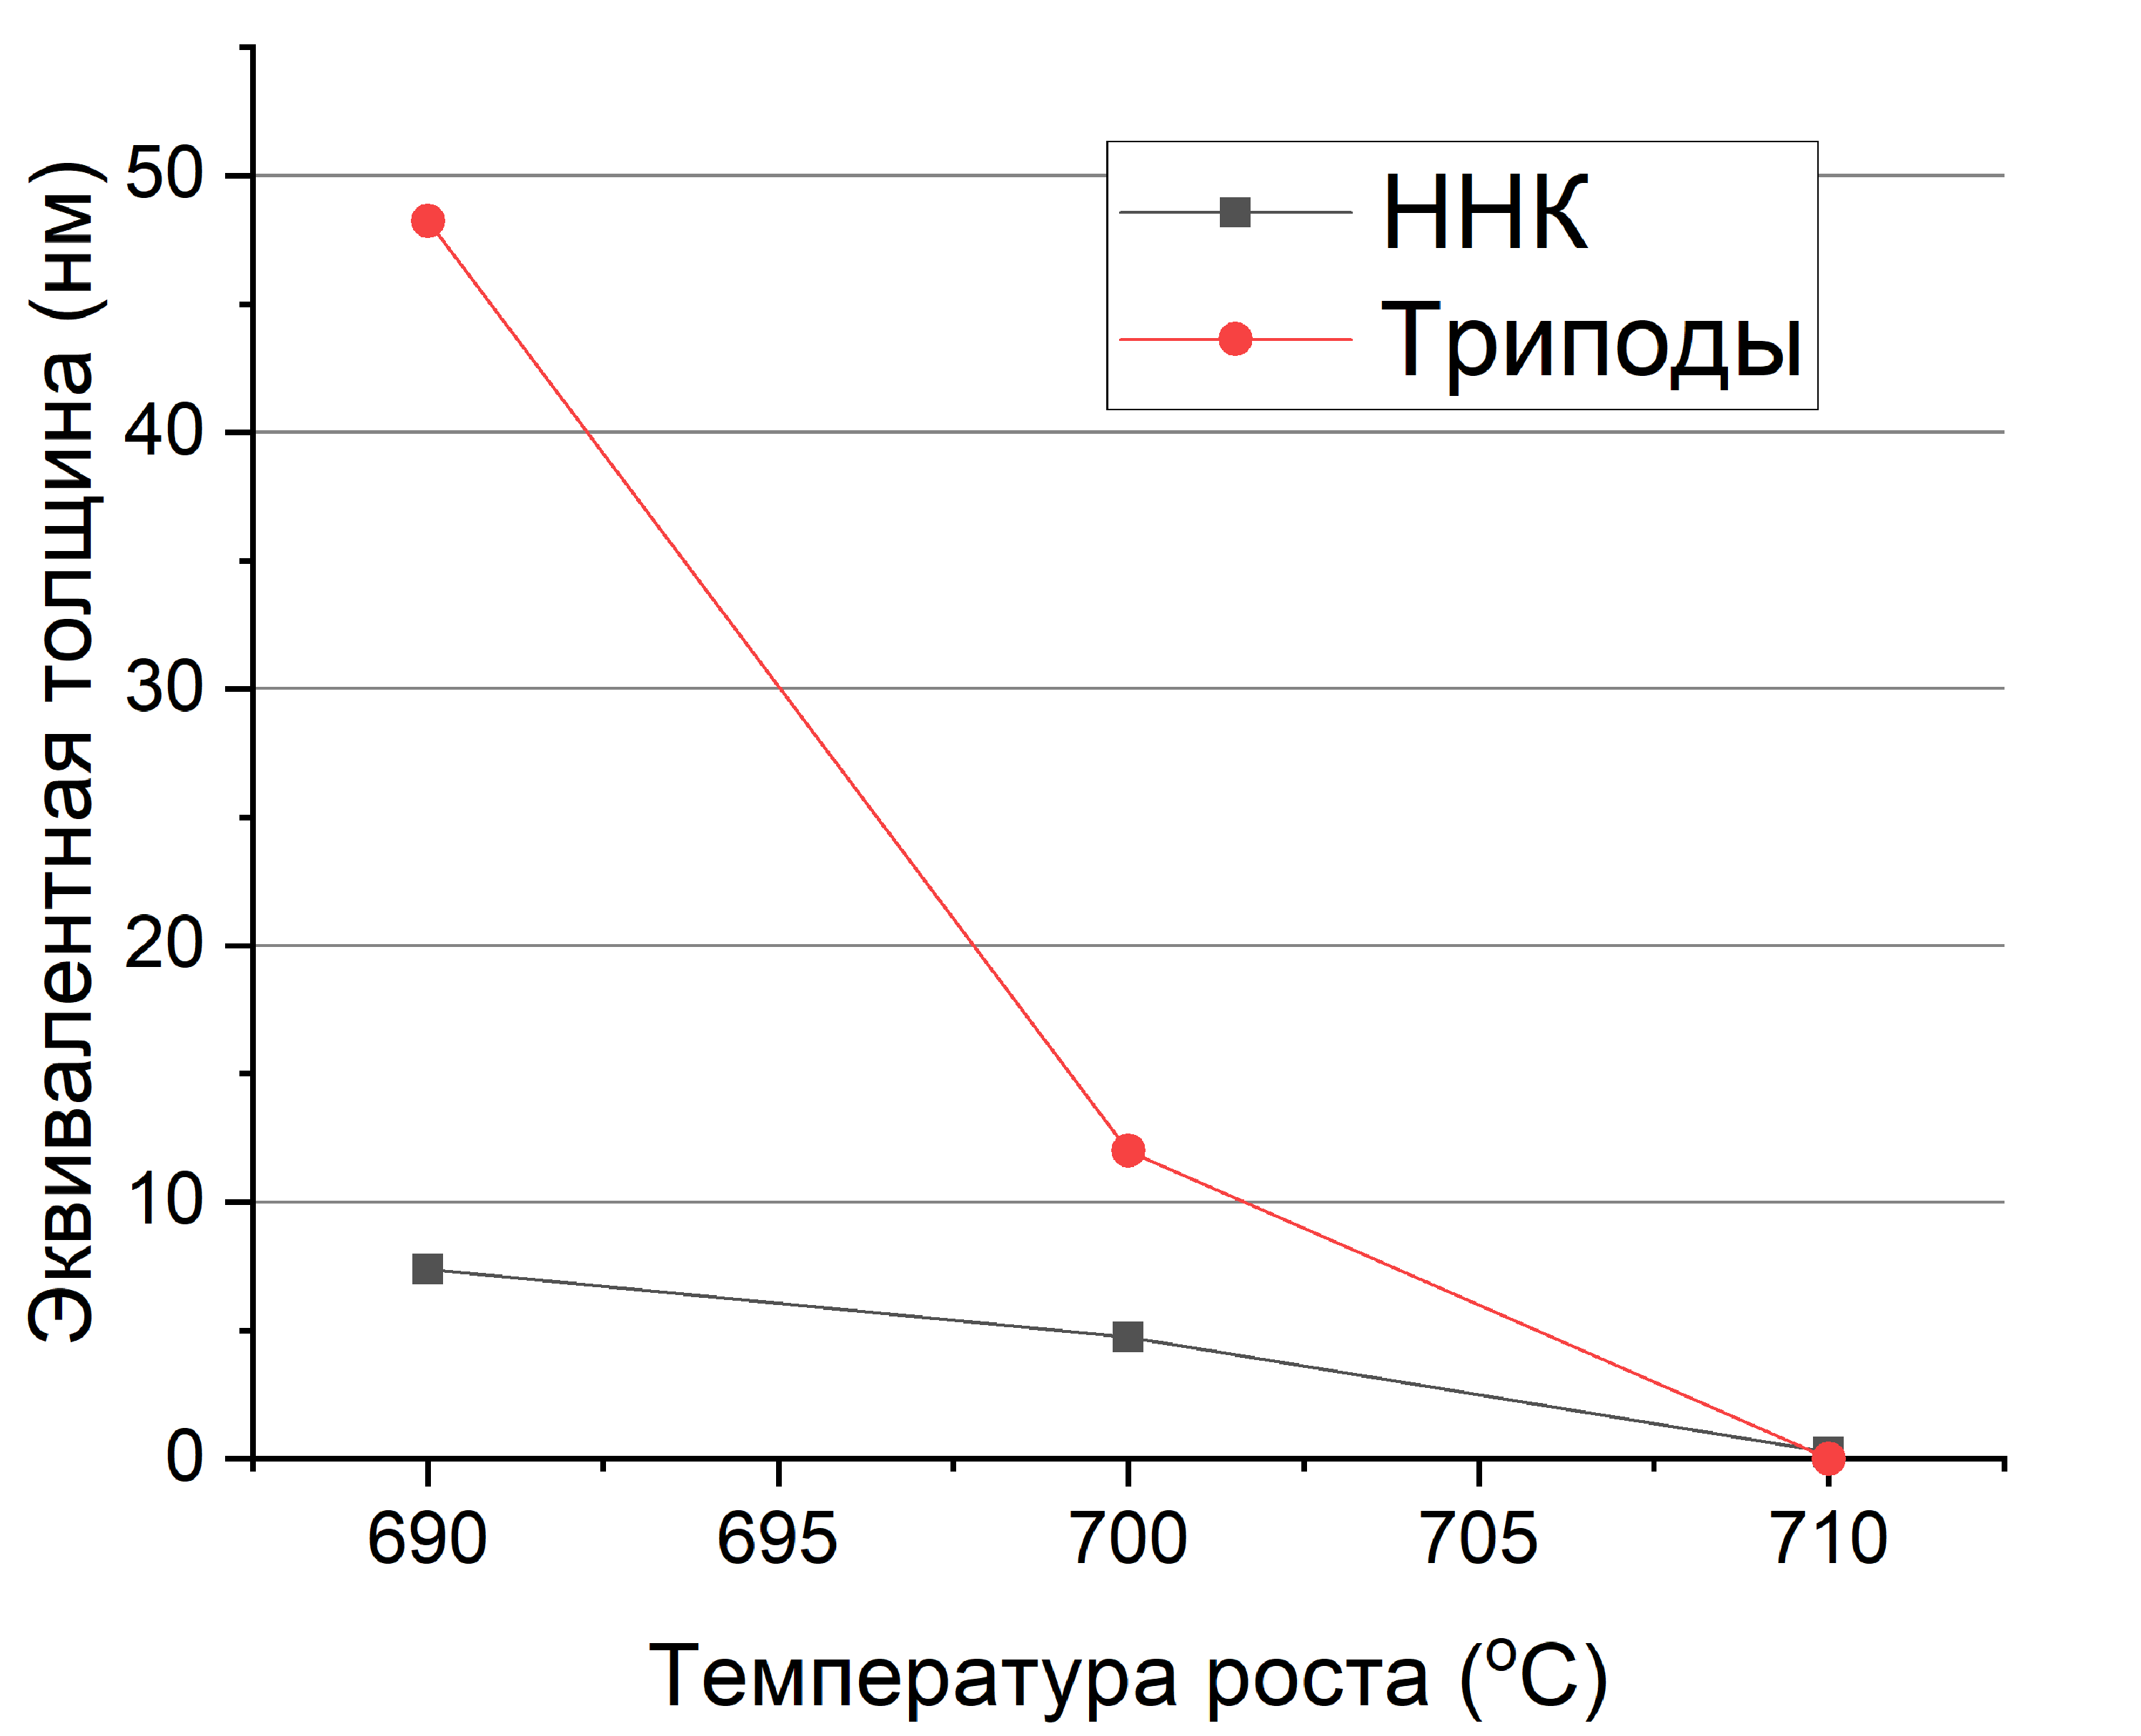
\includegraphics[width=0.48\linewidth]{Image_26_1_2}} }
			\caption{Зависимости поверхностной плотности~(а) и эквивалентной
		толщины~(б) наноструктур GaN от температуры роста}\label{fig:Image_26_1}
	\end{figure}

Эквивалентная толщина синтезированного материала и поверхностная плотность
наноструктур уменьшаются на порядок с повышением температуры с 690 до
710~\si{\degreeCelsius} (см.~рис.~\cref{fig:Image_26_1}). При температуре
700~\si{\degreeCelsius} формируются наиболее длинные ННК и наиболее крупные
триподы (см.~рис.~\cref{fig:Image_26_2}). Повышение температуры роста
увеличивает длину свободного пробега адатомов, что при 700~\si{\degreeCelsius}
приводит к увеличению аксиальной скорости роста. Можно предположить, что
снижение скорости роста наноструктур при дальнейшем повышении температуры
вызвано доминированием десорбции адатомов (см.~рис.~\cref{fig:Image_26_2}).

\begin{figure}[ht] \centerfloat{
	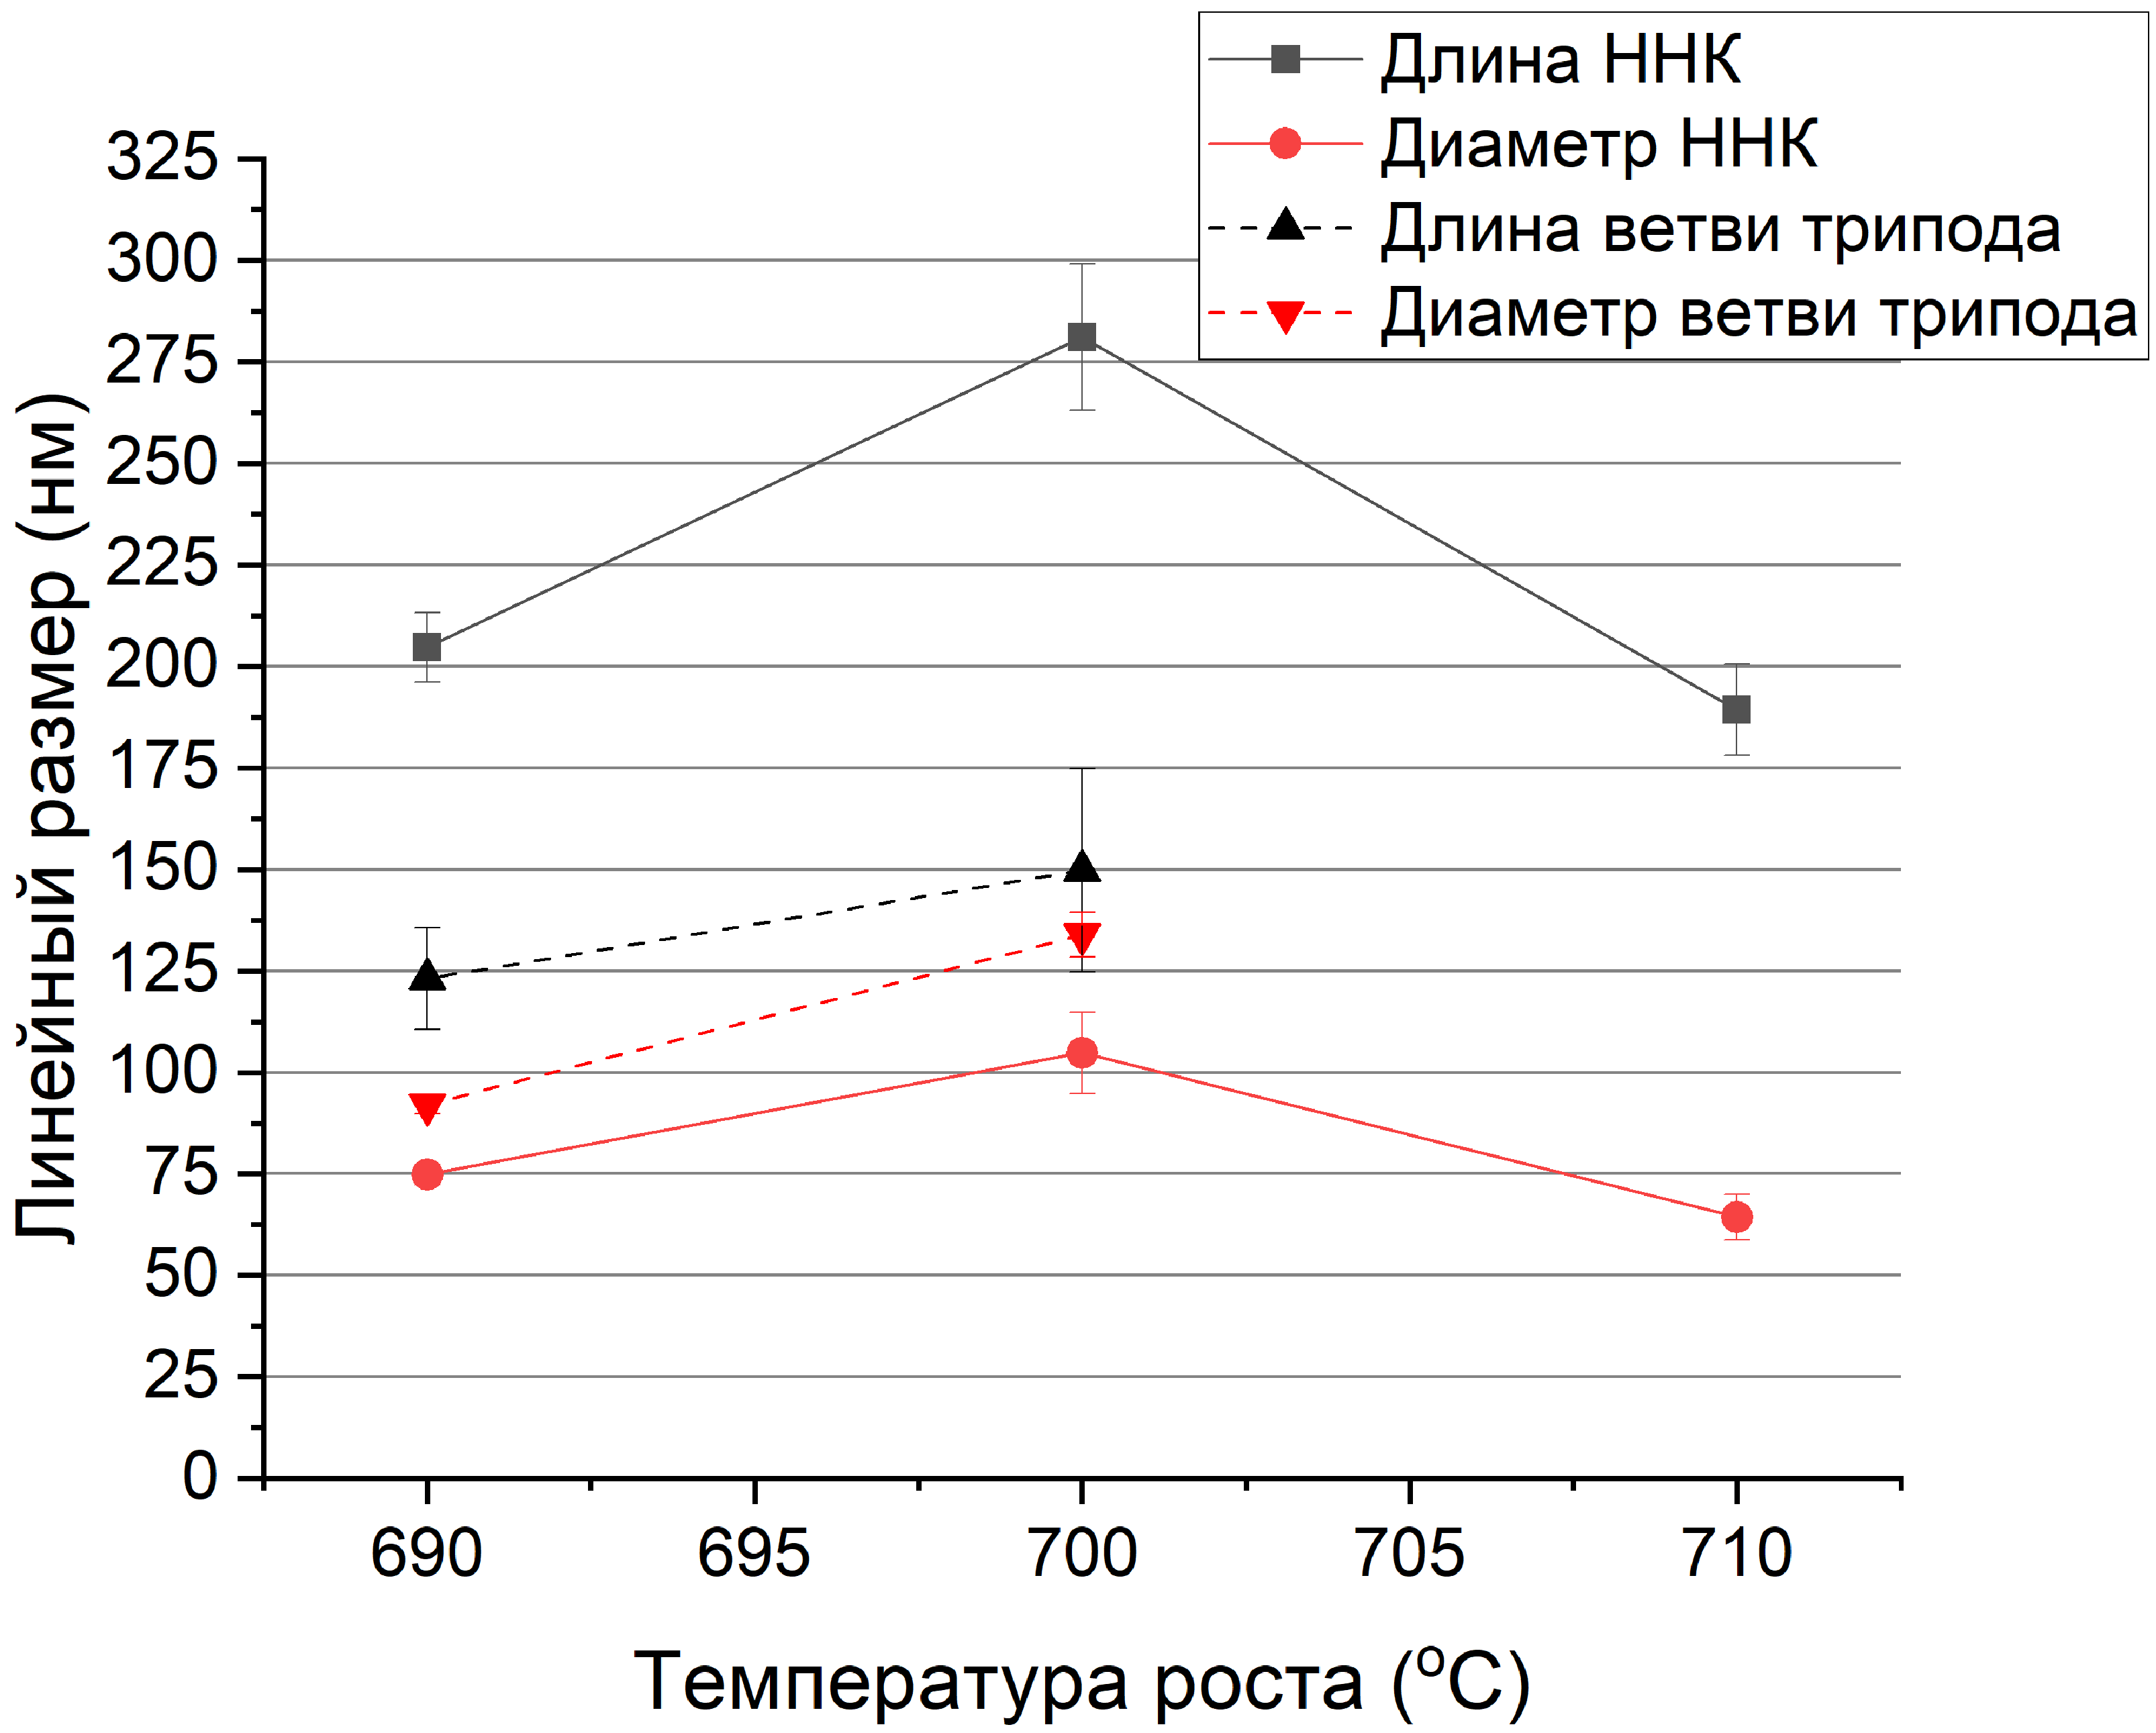
\includegraphics[width=0.6\linewidth]{Image_26_2} } \caption{Зависимости
линейных размеров наноструктур GaN от температуры роста}\label{fig:Image_26_2}
\end{figure}

Основание ННК имеет сужение к подложке. Угол вершины конуса основания ННК
(см.~рис.~\cref{fig:Image_25}) зависит от температуры и времени роста и лежит в
диапазоне от 20{\textdegree} до 42{\textdegree} (\(20\si{\degree} \pm
4\si{\degree}\) при температуре роста 710~\si{\degreeCelsius} и
\(42\si{\degree} \pm 2\si{\degree}\) при температуре роста
700~\si{\degreeCelsius}) \cite{Bolshakov2014}. Морфология ННК может зависеть от
положения подложки относительно источника \cite{Galopin2011}, поскольку оно
влияет на соотношение между молекулярными потоками, попадающими на боковые
стенки и верхнюю грань, таким образом оказывая влияние на длину свободного
пробега до встраивания адатомов Ga на боковых стенках. Это объясняет
зависимость от температуры: если источник азота расположен ортогонально
подложке~--- формируются GaN ННК с однородным по длине диаметром, а если под
острым (как в МПЭ установке Veeco GEN III)~--- ННК с утолщением.

\subsection{Влияние подготовки поверхности на морфологию массивов ННК}\label{sec:ch3/sec2/sub5}

Анализ изображений РЭМ синтезированных образцов~1--7 с массивами ННК
показывает, что все используемые буферные слои и методы подготовки подложки
приводят к образованию вертикально ориентированных ННК
(см.~рис.~\cref{fig:Image_27}), за исключением массива образца~1
(см.~рис.~\cref{fig:Image_27_1}) и выращенного на затравке из нанокапель Ga
(см.~рис.~\cref{fig:Image_27_4}). Наибольшей вертикальностью ННК обладают
массивы на смачивающих слоях Ga эквивалентной толщиной 0,3 и 0,6~монослоя
(образцы 5 (см.~рис.~\cref{fig:Image_27_5}) и 6
(см.~рис.~\cref{fig:Image_27_6})). Небольшой наклон оси роста ННК наблюдался у
массивов на буферном слое GaO\textsubscript{x} (образец 4
(см.~рис.~\cref{fig:Image_27_4})), необработанной (образец 1
(см.~рис.~\cref{fig:Image_27_1})) и нитридированной (образец 2
(см.~рис.~\cref{fig:Image_27_2})) подложках. На изображениях РЭМ
(см.~рис.~\cref{fig:Image_27}) наблюдается гексагональное поперечное сечение
ННК, что подтверждает их высокое кристаллическое совершенство. Численное
сравнение средней по времени осевой скорости роста, средних по длине ННК
диаметров и поверхностной плотности массивов ННК в зависимости от способа
подготовки подложки представлено на рисунке~\cref{fig:Image_28}.

\begin{figure}[ht] \centerfloat{ \subcaptionbox{\label{fig:Image_27_1}}{%
		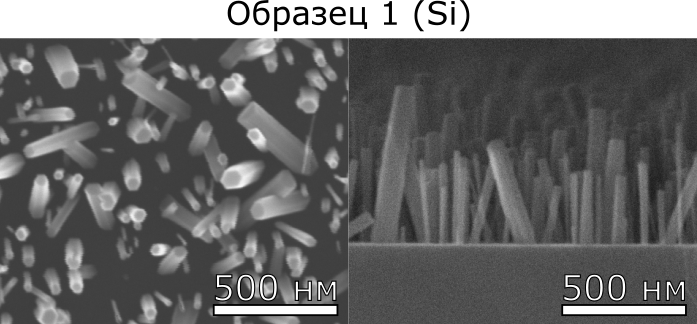
\includegraphics[width=0.45\linewidth]{Image_27_1}}

		\subcaptionbox{\label{fig:Image_27_2}}{%
			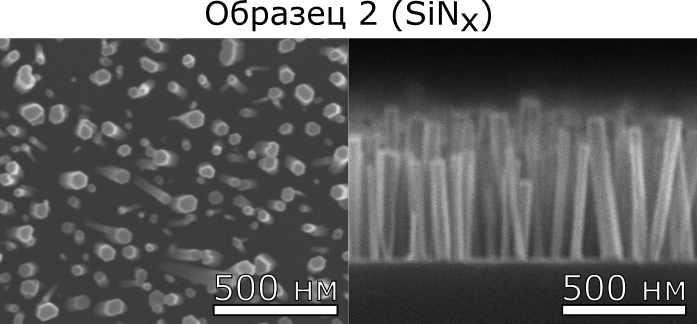
\includegraphics[width=0.45\linewidth]{Image_27_2}}
			\subcaptionbox{\label{fig:Image_27_3}}{%
			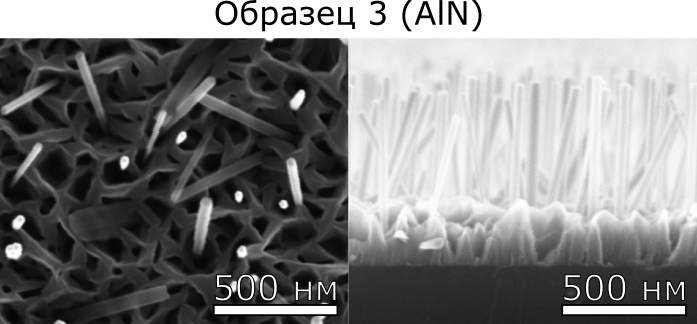
\includegraphics[width=0.45\linewidth]{Image_27_3}}

		\subcaptionbox{\label{fig:Image_27_4}}{%
			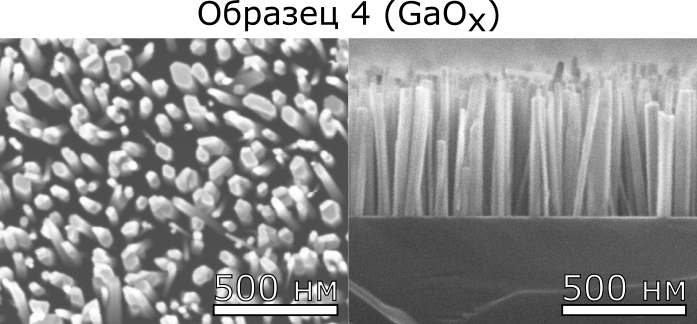
\includegraphics[width=0.45\linewidth]{Image_27_4}}
			\subcaptionbox{\label{fig:Image_27_5}}{%
			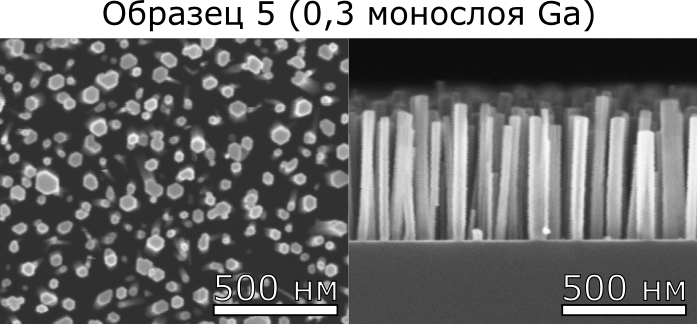
\includegraphics[width=0.45\linewidth]{Image_27_5}}

		\subcaptionbox{\label{fig:Image_27_6}}{%
			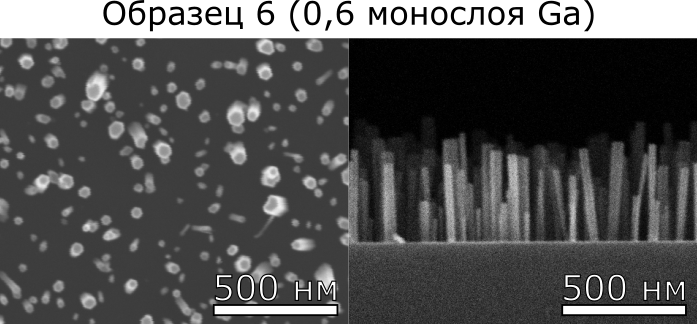
\includegraphics[width=0.45\linewidth]{Image_27_6}}
			\subcaptionbox{\label{fig:Image_27_7}}{%
			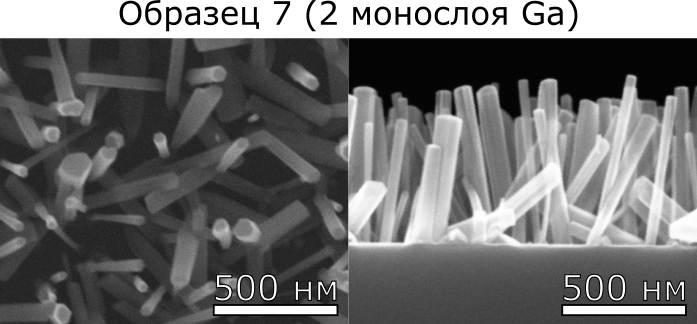
\includegraphics[width=0.45\linewidth]{Image_27_7}} }
			\legend{а)Образец~1: ННК, выращенные на Si, б) образец~2: на SiN, в)
				образец~3: на AlN, г) образец~4: на GaO\textsubscript{x}, д) образец~5:
				на 0,3~монослоях Ga, е) образец~6: на 0,6~монослоях Ga, ж) образец~7:
				на 2~монослоях Ga} \caption{РЭМ изображения синтезированных массивов
		GaN ННК}\label{fig:Image_27} \end{figure}

Согласно анализу РЭМ изображений, рост на необработанной подложке с
реконструкцией Si\((111)7\)\(\times\)\(7\) (образец~1) приводит к образованию
наименее однородного массива в серии по ориентации направлений роста ННК, а их
распределение осевых скоростей роста имеет самую высокую выборочную дисперсию.
Этот метод обеспечивает низкую по серии среднюю скорость осевого роста ННК
(22~\si{\nano\meter\per\hour}) со средним по серии диаметром
(48~\si{\nano\meter}).

Нитридация подложки перед осаждением GaN (образец~2) приводит к увеличению
поверхностной плотности ННК с 52 до 80~\si{\per\micro\meter\squared},
незначительному увеличению средней скорости осевого роста
(28~\si{\nano\meter\per\hour}), обеспечивает высокую ориентированность
синтезированных ННК.

Рост на буферном слое GaO\textsubscript{x} (образец~4) приводит к образованию
массива ННК с высокой поверхностной плотностью
(111~\si{\per\micro\meter\squared}) и высоким диаметром (65~\si{\nano\meter}),
что делает их перспективными для изготовления антиотражающих покрытий
\cite{Mozharov2015a}.

\begin{figure}[ht] \centerfloat{
		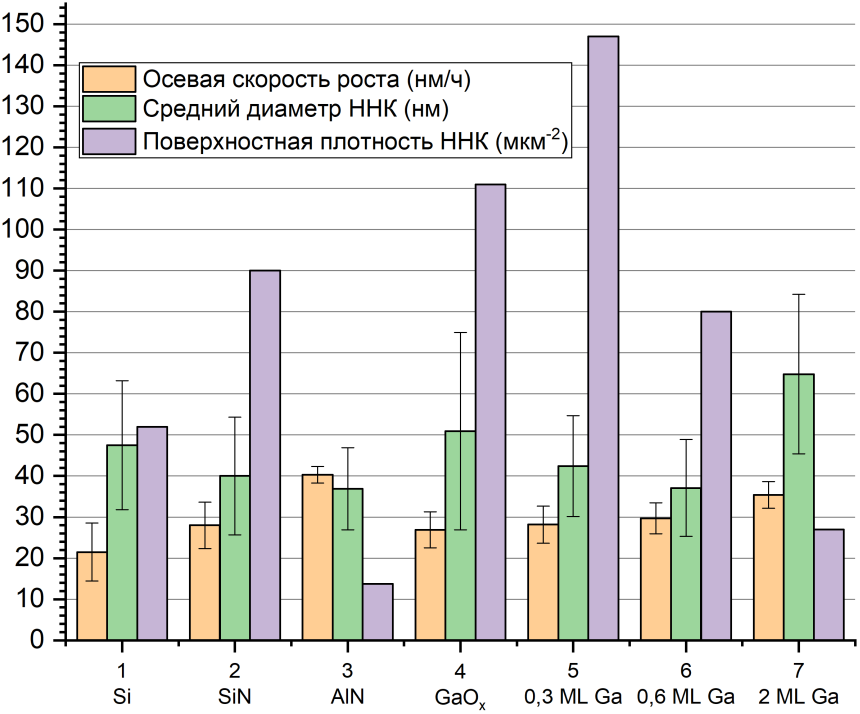
\includegraphics[width=0.7\linewidth]{Image_28} } \caption{Столбчатая
		диаграмма средней (по времени роста) осевой скорости роста, средних (по
		длине ННК) диаметров и поверхностной плотности массивов ННК GaN в
зависимости от метода обработки подложки}\label{fig:Image_28} \end{figure}

Использование смачивающего слоя Ga эквивалентной толщиной 0,3 и 0,6~монослоя
(образцы~5 и~6), нанесенного до нитридации Si, потенциально позволяет добиться
прямой гетерограницы GaN/Si. Анализ экспериментальных данных показывает, что
увеличение толщины слоя Ga приводит к снижению поверхностной плотности с 134 до
65~\si{\per\micro\meter\squared} (0,3~монослоя Ga и 0,6~монослоя Ga
соответственно).

Использование затравочного слоя Ga эквивалентной толщиной в 2 монослоя
значительно снижает поверхностную плотность ННК до
27~\si{\per\micro\meter\squared}, увеличивает средний диаметр
(65~\si{\nano\meter}) и скорость осевого роста (35~\si{\nano\meter\per\hour}).
Выращенные данным способом ННК обладают низкой ориентированностью, что
ограничивает их приборное применение.

Массив ННК, синтезированный на затравке AlN (образец~3) имеет наименьшую
поверхностную плотность (14~\si{\per\micro\meter\squared}) и наибольшую среднюю
скорость осевого роста ННК (40~\si{\nano\meter\per\hour}). При этом длины ННК
имеют наименьшую выборочную дисперсию. В этом случае зарождение ННК обусловлено
наличием N-полярных островков AlN. Наряду с этим Ga-полярная сетка GaN наностен
покрывает Al-полярный слой AlN, который занимает большую долю поверхности
образца \cite{Auzelle2015}.

Полученные изображения картин ДБЭ для различных азимутальных направлений в
конце роста ННК представлены на~рис.~\cref{fig:Image_29}. Наблюдаемые картины
ДБЭ от ННК соответствуют кристаллической структуре WZ. В работе
\cite{Wierzbicka2013} отмечается сохранение следующих эпитаксиальных отношений
для ННК GaN на Si:
(0001)\textsubscript{GaN}\(\parallel\)(111)\textsubscript{Si} и
<\(112\overline{0}\)>\textsubscript{GaN}\(\parallel\)<\(11\overline{0}\)>\textsubscript{Si}.
На изображениях ДБЭ (см.~рис.~\cref{fig:Image_29}) наблюдается различное
распределения эпитаксиальных ориентаций в зависимости от метода подготовки
поверхности подложки. Наклон ННК наблюдается на РЭМ изображениях ННК GaN,
выращенных на необработанном Si (см.~рис.~\cref{fig:Image_29_1}) и
предварительно нитридированном Si (см.~рис.~\cref{fig:Image_27_2}). Наиболее
низкая дисперсия распределения углов наклона ННК наблюдается на образце с
затравкой AlN (образец~3 (см.~рис.~\cref{fig:Image_27_3})). На образце~7
(2~монослоя Ga) (см.~рис.~\cref{fig:Image_27_7}) присутствуют случайно
наклонённые ННК на угол до 60{\textdegree} к нормали подложки. Это
соответствует наклону оси <0001>\textsubscript{GaN}, который отражается на
картинах ДБЭ поперечным уширением штрихов брэгговских рефлексов.

\begin{figure}[ht] \centerfloat{ \subcaptionbox{\label{fig:Image_29_1}}{%
			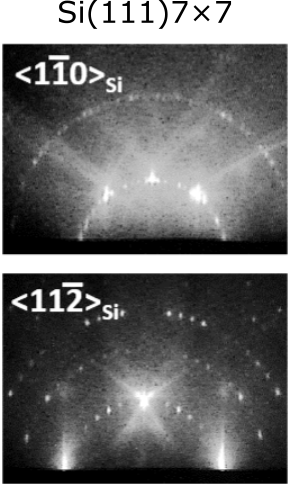
\includegraphics[width=0.2\linewidth]{Image_29_1}}
			\subcaptionbox{\label{fig:Image_29_2}}{%
				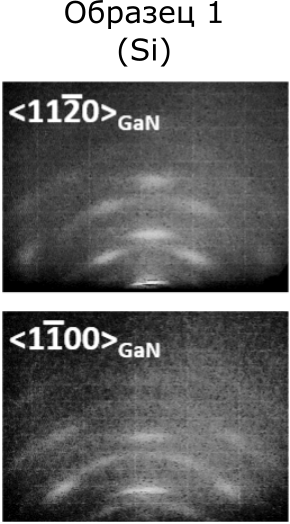
\includegraphics[width=0.2\linewidth]{Image_29_2}}
				\subcaptionbox{\label{fig:Image_29_3}}{%
					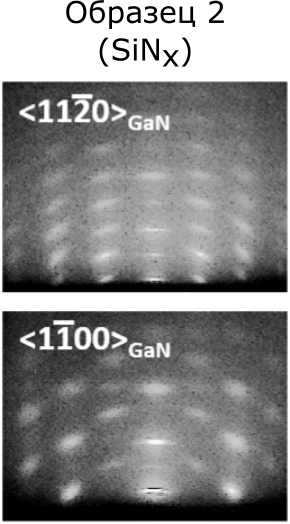
\includegraphics[width=0.2\linewidth]{Image_29_3}}
					\subcaptionbox{\label{fig:Image_29_4}}{%
					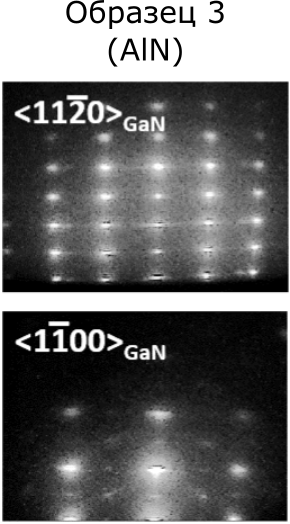
\includegraphics[width=0.2\linewidth]{Image_29_4}}

		\subcaptionbox{\label{fig:Image_29_5}}{%
			\includegraphics[width=0.2\linewidth]{Image_29_5}}
			\subcaptionbox{\label{fig:Image_29_6}}{%
				\includegraphics[width=0.2\linewidth]{Image_29_6}}
				\subcaptionbox{\label{fig:Image_29_7}}{%
				\includegraphics[width=0.2\linewidth]{Image_29_7}}
				\subcaptionbox{\label{fig:Image_29_8}}{%
				\includegraphics[width=0.2\linewidth]{Image_29_8}} } \legend{Картины
				ДБЭ сняты в направлениях  <\(1\overline{1}0\)>\textsubscript{Si} и
				<\(11\overline{2}\)>\textsubscript{Si}} \caption{Картины ДБЭ
				Si\((111)7\)\(\times\)\(7\), полученные до роста ННК GaN~(а) и в конце
				роста ННК на различных подготовленных поверхностях~(б --
		и)}\label{fig:Image_29} \end{figure}

Поперечное уширения брэгговских рефлексов не наблюдалось для образца~3 (AlN)
(см.~рис.~\cref{fig:Image_29_4}). Как видно из соответствующих РЭМ изображений
(см.~рис.~\cref{fig:Image_27_3}), на этом образце наблюдается паразитное
образование сплошного слоя GaN, образованного сеткой наностен. Это явление
связано с влиянием затравочных островков AlN на зарождение и полярность GaN
\cite{Zhong2018}. Можно предположить, что низкая поверхностная плотность
массива ННК приводит к преобладанию дифракции от сетки наностен при
формировании картины ДБЭ.

За исключением образца~3 (AlN), наиболее четкая картина ДБЭ наблюдается от
массива образца~5 (0.3 монослоя Ga), что свидетельствует о его высоком
кристаллическом совершенстве (см.~рис.~\cref{fig:Image_29_6}). Наиболее
уширенные рефлексы ДБЭ наблюдаются от массива образца~1 (без дополнительной
обработки), что указывает на наклон и несогласованность кристаллической
ориентации ННК в плоскости подложки.

Картина ДБЭ массива образца~4 (GaO\textsubscript{x})
(см.~рис.~\cref{fig:Image_29_5}) полностью независима от азимутальной
ориентации образца, что указывает на мозаичность кристаллографической
ориентации ННК в плоскости подложки, вызванный микрокристалличностью затравки
GaO\textsubscript{x}.

Высокая дисперсия кристаллических ориентаций ННК в плоскости подложки
наблюдаются в массиве образца~7, выращенном на затравке нитридированных капель
Ga эквивалентной толщиной в 2 монослоя (см.~рис.~\cref{fig:Image_27_7}). В
главе~\cref{ch:ch3} обсуждалась нитридация Ga капель и тот факт, что она может
привести к образованию наночастиц ZB-GaN с \{111\}\textsubscript{GaN} гранями,
действующими в качестве центров зародышеобразования для роста ННК
\cite{Fedorov2018}. В этом случае ориентация решётки ННК зависит от
кристаллического качества и ориентации затравок ZB-GaN. Картины ДБЭ от массива
данного образца, снятые вдоль перпендикулярных направлений
<\(1\overline{1}0\)>\textsubscript{Si} и <\(11\overline{2}\)>\textsubscript{Si}
(см.~рис.~\cref{fig:Image_29_8}) схожи, а полукруглое удлинение рефлексов ДБЭ
указывает на высокую мозаичность кристаллографических ориентаций ННК в
плоскости подложки.

\subsection{Влияние подготовки поверхности на низкотемпературную ФЛ ННК}\label{sec:ch3/sec2/sub6}

На~рис.~\cref{fig:Image_30_1} приведены спектры ФЛ, полученные при температуре
5~\si{\kelvin} с использованием гелиевого криостата с замкнутым циклом. В
спектрах не наблюдается характерной жёлтой линии ФЛ, связанной с высокой
плотностью дефектных состояний \cite{Suski1995}. Все образцы имеют две основные
линий ФЛ с энергиями \(\approx 3,468\)~\si{\electronvolt} и \(\approx
3,472\)~\si{\electronvolt} (обозначены на~рис.~\cref{fig:Image_30_1} линиями a
и b), соответствующие рекомбинации экситонов, связанных на нейтральных донорах
(D\textsubscript{0}~X) (donor bound exciton, DBE) \cite{Bolshakov2018,
Paskov2004}. Полуширина линий \(\approx 4,5\)~\si{\milli\electronvolt} не
позволяет разрешить пики от рекомбинации экситонов на легирующих примесях
кислорода (O\textsuperscript{0},~X\textsuperscript{A}) и кремния
(Si\textsuperscript{0},~X\textsuperscript{A}) \cite{Zettler2015}, однако стоит
полагать, что (Si\textsuperscript{0},~X\textsuperscript{A}) переходы вносят
больший вклад в сигнал ФЛ из-за преднамеренного Si легирования в течение
последних нескольких часов роста до концентрации
10\textsuperscript{19}~\si{\per\centi\metre\cubed}. В данной работе не
исследовалось пространственное распределение легирующей примеси, однако, нижняя
часть ННК также может быть легирована Si из-за радиального роста и объёмной
диффузии атомов Si на гетерогранице с кремниевой подложкой. По этим причинам
экситоны, связанные на акцепторе, в исследуемых образцах не ожидаются.
Появление линий a и b может быть вызвано донорно связанными тяжело-
(D\textsuperscript{0},~X\textsuperscript{B}) и лёгкодырочными
(D\textsuperscript{0},~X\textsuperscript{A}) экситонными переходами. Другая
возможная причина расщепления DBE связана с поверхностными эффектами
\cite{Calarco2011}, влияющими на энергию связи экситон\,--\,донор или
вызывающими неоднородность концентрации легирующей примеси, так как излучение
DBE может испытывать красное смещение на \(\approx 6\)~\si{\milli\electronvolt}
при увеличении концентрации легирующей примеси Si на порядок (c
10\textsuperscript{17} до 10\textsuperscript{18}~\si{\per\centi\metre\cubed})
\cite{Pozina2011}.

\begin{figure}[ht] \centerfloat{
\includegraphics[width=0.6\linewidth]{Image_30_1} } \caption{Низкотемпературные
спектры ФЛ синтезированных массивов ННК GaN}\label{fig:Image_30_1} \end{figure}

Высокоэнергетическое плечо спектра ФЛ (линия c на~рис.~\cref{fig:Image_30_1})
может быть связано с рекомбинацией экситонов со свободной дыркой
(X\textsuperscript{A},~X\textsuperscript{B}) (free hole exciton, FE).

Спектры ФЛ имеют различную интенсивность и ширину линий в зависимости от метода
подготовки ростовой поверхности, что может быть вызвано структурными
нарушениями, различием в морфологии массивов ННК. Низкая интенсивность ФЛ от
массивов образца~4 (GaO\textsubscript{x}) и образца~6 (0,6~монослоя Ga) может
быть связана с многочисленным слиянием ННК, и вызванными им протяжёнными
дефектами упаковки, что подтверждается уширением рефлексов на картинах ДБЭ.
Наименьшую интенсивность сигнала ФЛ имеет массив образца~7 (2~монослоя Ga).
Остальные образцы (за исключением образца~3 (AlN)) имеют близкие интенсивности
ФЛ. Спектр ФЛ от массива образца~2 (SiN) имеет наиболее интенсивную
коротковолновую линию c и слабую DBE линию b. Такое различие может быть вызвано
низким уровнем легирования, так как нитридация поверхности подложки может
препятствовать объёмной диффузии Si из подложки в растущий ННК. Образец~1 и
образец~5 (0,3~монослоя Ga) имеют схожую форму спектра ФЛ и близкое отношение
интенсивностей линий a/b, аналогично образцу~4 (GaO\textsubscript{x}), однако
он может иметь отличный механизм ФЛ из-за непреднамеренного легирования
кислородом.

Наибольшая интенсивность ФЛ была получена от образца~3 (AlN): низкая
поверхностная плотность позволяет избежать слияния ННК и связанных с ним
структурных дефектов, что уменьшает вероятность безызлучательной рекомбинации и
позволяет добиться высокой интенсивности сигнала ФЛ. Спектр ФЛ обладает низким
отношениями интенсивностей a/b-линий. ННК массива обладают аналогичными
поперечными размерами и самой высокой скоростью осевого роста среди образцов,
что при постоянном потоке Si легирующей примеси приводит к меньшей объёмной
концентрации доноров. Как видно на РЭМ изображениях
(см.~рис.~\cref{fig:Image_27_3}), на подложке Si присутствует слой объёмного
материала сетки наностен GaN высотой 200~\si{\nano\meter}. В данный слой также
встраиваются адатомы легирующей примеси, что значительно снижает уровень
легирования и может объяснить различие в сигнале ФЛ. Чтобы удалить ННК с
подложки (см. вставку на~рис.~\cref{fig:Image_30_2}) и изучить вклад объёмного
слоя в интенсивность ФЛ поверхность подложки была механически процарапана с
последующей обработкой образца в ультразвуковой ванне.

\begin{figure}[ht] \centerfloat{
		\includegraphics[width=0.6\linewidth]{Image_30_2} } \legend{На вставке РЭМ
		изображение образца~3 (AlN) после удаления ННК, масштабная метка
		400~\si{\nano\meter}} \caption{Низкотемпературные спектры ФЛ образца 3
		(AlN), полученные до (красная кривая) и после (чёрная кривая) удаления
ННК}\label{fig:Image_30_2} \end{figure}

Интенсивность низкотемпературной ФЛ (см.~рис.~\cref{fig:Image_30_2}) после
удаления ННК составляет \(\approx 40\,\%\) от первоначальной. Можно
предположить, что планарные слои GaN, выращенные на подложке Si, имеют низкую
эффективность ФЛ из-за безызлучательной рекомбинацией на дефектах, вызванных
рассогласованием решёток \cite{Calleja1999, Reshchikov2005}.

\section{Основные результаты}\label{sec:ch3/sec3}

Продемонстрирован эпитаксиальный синтез методом ПА-МПЭ наноструктур и в форме
GaN ННК и триподов на Si(111) подложке с предварительным формированием
затравочных наноостровков GaN. После нитридации наноостровки приобретают
кольцеобразную форму. Данные островки имеют ZB структуру и впоследствии
находятся в основе триподов и наклонённых ННК.

Поверхностная плотность, размер и аспектное отношение структур можно
контролировать температурой роста, потоком III группы и эквивалентной толщиной
затравочного слоя. Нуклеация триподов может быть полностью подавлена путем
уменьшения эквивалентной толщины затравки Ga и повышения температуры роста выше
710~\si{\degreeCelsius}.

Направление ветвей соответствует кристаллографическому направлению
<\(0001\)>\textsubscript{GaN} с преимущественной ориентацией вдоль направлений
<\(1\overline{1}0\)>\textsubscript{Si}, <\(11\overline{2}\)>\textsubscript{Si}
и \(<12\overline{3}>\)\textsubscript{Si}. Плоскость
\((11\overline{2}1)\)\textsubscript{GaN} триподов имеет эпитаксиальное
отношение с параллельной плоскостью подложки (111)\textsubscript{Si}.

Спектр ФЛ от массив нанотриподов с включениями политипа ZB имеет три полосы:
интенсивную полосу, характерную для объёмного WZ-GaN (\(\approx
3,48\)~\si{\electronvolt}), полосу, характерную для GaN с дефектами упаковки
(\(\approx 3,43\)~\si{\electronvolt}) и полосу, характерную для ZB-GaN
(\(\approx 3,25\)~\si{\electronvolt}).

Исследовано эпитаксиальное формирование ННК GaN на обработанной различными
методами подложке Si(111): нитридированной в активированном азоте с
образованием слоя SiN\textsubscript{x}, с буферным слоем GaO\textsubscript{x},
с затравочными островками AlN и GaN, со смачивающими слоями Ga эквивалентной
толщиной 0,3 и 0,6~монослоя. Показано, как подготовка ростовой поверхности
влияет на морфологию и оптические свойства ННК GaN. Наиболее однородный по
длине ННК массив был получен на буферном слое AlN, а наименее однородный массив
получен на необработанной подложке. Вертикальный массив ННК со случайными
кристаллическими ориентациями в плоскости подложки был получен на
микрокристаллическом широкозонном полупроводниковом буферном слое
GaO\textsubscript{x}.

На спектрах ФЛ от синтезированных образцов наблюдается интенсивный сигнал,
обусловленный рекомбинацией экситонов, связанных на нейтральных донорах.
Наибольшая интенсивность ФЛ наблюдается от массива ННК на AlN, а наименьшая~---
от массива на наноостровках GaN, полученных после нитридации капель Ga.

Высокая дисперсия средней по времени осевой скорости роста и низкая
ориентированность ННК массива образца~1 может быть обусловлена поверхностной
неоднородностью из-за нитридации Si, которая начинается одновременно с ростом
GaN и продолжается во время роста.

В случае с AlN затравкой её формирование путём нитридации Al капель на высоких
температурах может привести к дополнительной поверхностной неоднородности,
вызванной локальным легированием подложки из-за растворимости Al в Si. Самая
высокая скорость осевого роста ННК GaN на затравке AlN и самая высокая
интенсивность ФЛ среди всех исследованных методов делают данный ростовой метод
привлекательным для создания оптоэлектронных приборов.

Использование затравочного слоя нанокапель Ga эквивалентной толщиной 2 монослоя
приводит к росту однородных по длине наклонных ННК. Учитывая, что нитридация
капель Ga приводит к образованию наноостровков ZB-GaN, можно предположить, что
неоднородность ориентаций ННК определяется подготовкой наноостровков: размером
и поверхностной плотностью капель Ga, условиями нитридации. В неоптимальных
условиях роста может происходить двойникование (вращение на 180{\textdegree}
вокруг всех возможных направлений <111>) кристаллической решётки наночастиц
ZB-GaN, приводящее к случайной ориентации их граней
\{111\}\textsubscript{ZB-GaN} и, следовательно, случайной ориентации
зародившихся на этих гранях ННК. Данный образец имеет наименьшую интенсивность
сигнала ФЛ из-за наличия дефектов при слиянии наклонных ННК.

В случае однородной поверхности роста дисперсия размеров и скорость роста ННК в
основном определяются диффузией и десорбцией адатомов. Поэтому формирование
вертикальных массивов ННК на GaO\textsubscript{x} может быть объяснено с точки
зрения механизма самоиндуцированного роста, обусловленного анизотропией
поверхностных энергий и диффузией адатомов Ga и N, а не влиянием ориентации
подложки или кристаллической структуры \cite{Sobanska2016}.
Поликристалличность GaO\textsubscript{x} приводит к случайной ориентации в
плоскости подложки, а наличие однородной гладкой поверхности
GaO\textsubscript{x} определяет вертикальность массивов GaN ННК.

Морфология массивов ННК, выращенных на нитридированной поверхности
(111)\textsubscript{Si} и поверхности с эквивалентной толщиной Ga в 0,6
монослоя, весьма схожа, а массив на смачивающем слое Ga эквивалентной толщиной
0,3 монослоя имеет поверхностную плотность ННК почти в два раза выше.

\FloatBarrier
